% PT
%\documentclass[phd,twoside,brazil]{ThesisPUC}
\documentclass[phd,twoside,british]{ThesisPUC_uk}

\usepackage{verbatim}
\usepackage{xspace}
\usepackage{graphicx}
\usepackage{multirow}
\usepackage{alltt}

\usepackage[T1]{fontenc}
%\usepackage{lmodern}
%\usepackage[utf8]{inputenc}

\usepackage{amssymb}
\usepackage{amsmath}
\usepackage{amsfonts}
\usepackage{amsthm}
\usepackage{mathtools}
\usepackage{dsfont}

\usepackage{color}
\usepackage{xcolor,colortbl}
\definecolor{light}{gray}{0.90}
\definecolor{dark}{gray}{0.30}
%\definecolor{light}{rgb}{.90,.90,.90}
\definecolor{darkgreen}{rgb}{0,.50,0}
\definecolor{darkblue}{rgb}{0,0,.50}
\definecolor{darkred}{rgb}{.50,0,0}
\definecolor{darkpur}{rgb}{.50,0,.50}
\usepackage{listings}
\lstset{
%columns=fullflexible,
%basicstyle=\ttfamily,
escapeinside={||},
mathescape=true,
    language=C, % choose the language of the code
    basicstyle=\fontfamily{pcr}\selectfont\footnotesize\color{black},
    keywordstyle=\color{black}\bfseries, % style for keywords
    numbers=none, % where to put the line-numbers
    numberstyle=\tiny, % the size of the fonts that are used for the line-numbers
    backgroundcolor=\color{light},
    %showspaces=false, % show spaces adding particular underscores
    %showstringspaces=false, % underline spaces within strings
    showtabs=false, % show tabs within strings adding particular underscores
    %frame=single, % adds a frame around the code
    tabsize=2, % sets default tabsize to 2 spaces
    %rulesepcolor=\color{gray}
    captionpos=t, % sets the caption-position to bottom
    breaklines=false, % sets automatic line breaking
    %breakatwhitespace=false,
    numbersep=2em,
    emph={par,or,do,end,loop,await,emit,input,event,call,with,command,%
          var,and,not,then,else,native,return,pure,safe,nohold,finalize,%
          fin,mem,nop,PROC,PAR,CHAN,SIGNAL,async,sync,class,module,output,%
          each,foreach,every,abort,when},
    emphstyle={\bfseries},
    commentstyle=\color{dark},
    %xleftmargin=20pt,
    %xrightmargin=20pt,
    framesep=20pt,
    %upquote=true,
    %aboveskip={1.5\baselineskip},
}

\newcommand{\code}[1] {{\small{\texttt{#1}}}}
\newcommand{\Code}[1] {\texttt{#1}}

\newcommand{\CEU}{\textsc{C\'{e}u}\xspace}
\newcommand{\nesc}{\emph{nesC}\xspace}
\newcommand{\FIN}{\code{finally}\xspace}
\newcommand{\DOFIN}{\code{do-finally}\xspace}

\newcommand{\footnoteremember}[2]{%
\footnote{#2}%
\newcounter{#1}%
\setcounter{#1}{\value{footnote}}%
}
\newcommand{\footnoterecall}[1]{%
\footnotemark[\value{#1}]%
}

\newcommand{\ST}{\1\xrightarrow[~n~]{}\1}
\newcommand{\BT}{\xRightarrow[(i,E)]{}}
\newcommand{\LL}{\langle}
\newcommand{\RR}{\rangle}
\newcommand{\DS}{\displaystyle}

\newcommand{\1}{\;}
\newcommand{\2}{\;\;}
\newcommand{\3}{\;\;\;}
\newcommand{\5}{\;\;\;\;\;}
\newcommand{\ten}{\5\5}
\newcommand{\twenty}{\ten\ten}

\definecolor{dark-red}{rgb}{0.2,0.15,0.15}
\definecolor{dark-blue}{rgb}{0.15,0.15,0.4}
\definecolor{medium-blue}{rgb}{0,0,0.5}
% PT
\hypersetup{
    colorlinks, linkcolor={dark-red},
    citecolor={dark-blue}, urlcolor={medium-blue}
}
%\usepackage[hidelinks]{hyperref}
%\hypersetup{hidelinks=true}
%\hypersetup{frenchlinks=true}

%%%%%%%%%%%%%%%%%%%%%%%%%%%%%%%%%%%%%%%%%%%%%%%%%%%%%%%%%%%%%%%%%%%%%%%%%%%%%%%%

\author{Francisco Figueiredo Goytacaz Sant'Anna}
\authorR{Sant'Anna, Francisco Figueiredo Goytacaz}
\adviser{Roberto Ierusalimschy}
\adviserR{Ierusalimschy, Roberto}
\coadviser{Noemi de La Roque Rodriguez}
\coadviserR{Rodriguez, Noemi de La Roque}

% PT
%\titulo{
%Concorr\^encia Segura em n\'ivel de Sistema para N\'os com Restri\c{c}\~oes de 
%Recursos com C\'eu
%}

\title{Safe System-Level Concurrency on Resource-Constrained Nodes with C\'eu}

\day{12} \month{September} \year{2013}

\city{Rio de Janeiro}
\CDD{004}
\department{Inform\'atica}
\program{Computer Science}
\school{Centro T\'{e}cnico Cient\'{i}fico}
\university{Pontif\'{i}cia Universidade Cat\'{o}lica do Rio de Janeiro}
\uni{PUC--Rio}

%%%%%%%%%%%%%%%%%%%%%%%%%%%%%%%%%%%%%%%%%%%%%%%%%%%%%%%%%%%%%%%%%%%%%%%%%%%%%%%%

\jury {
    %\jurymember{Edward Hermann Haeusler}
                %{Departamento de Inform\'{a}tica --- PUC-Rio}
    %\jurymember{Renato Fontoura de Gusm\~{a}o Cerqueira}
                %{Departamento de Inform\'{a}tica --- PUC-Rio}
    %\schoolhead{Jos\'{e} Eugenio Leal}
}

%%%%%%%%%%%%%%%%%%%%%%%%%%%%%%%%%%%%%%%%%%%%%%%%%%%%%%%%%%%%%%%%%%%%%%%%%%%%%%%%

\resume {
}


%%%%%%%%%%%%%%%%%%%%%%%%%%%%%%%%%%%%%%%%%%%%%%%%%%%%%%%%%%%%%%%%%%%%%%%%%%%%%%%%

\acknowledgment{
I would like to thank my supervisors Roberto Ierusalimschy and Noemi Rodriguez 
for their time and knowledge.

%TTT: Olaf / Philippas / Cerqueira

I'm also thankful to Luiz Fernando Soares, for my period in the Telem\'idia 
Lab, and all my teachers in CAp-UERJ, responsible for my education before 
college.

My studies were funded by CNPq and SAAB.
}


%%%%%%%%%%%%%%%%%%%%%%%%%%%%%%%%%%%%%%%%%%%%%%%%%%%%%%%%%%%%%%%%%%%%%%%%%%%%%%%%

% PT
\begin{comment}
\keywords {
    \key{Concorr\^encia}
    \key{Determinismo}
    \key{Sistemas Embarcados}
    \key{Esterel}
    \key{S\'incrono}
    \key{Reativo}
    \key{Redes de Sensores sem Fio}
}
\end{comment}

%\begin{comment}
\keywords{
  \key{Concurrency}%
  \key{Determinism}%
  \key{Embedded Systems}%
  \key{Esterel}%
  \key{Reactivity}%
  \key{Synchronous}%
  \key{Wireless Sensor Networks}%
}
%\end{comment}

% TODO muito corrido

%\begin{comment}
\abstract {
% TODO: split 2 sents.
Despite the continuous research to facilitate Wireless Sensor Networks 
development,
most safety analysis and mitigation efforts in concurrency are still left to 
developers, who must manage synchronization and shared memory explicitly.
% among activities explicitly.
%
We propose a system language that ensures safe concurrency by handling threats 
at compile time, rather than at runtime.
%
The synchronous and static foundation of our design allows for a simple 
reasoning about concurrency that enables compile-time analysis resulting in
deterministic and memory-safe programs.
%
As a trade-off, our design imposes limitations on the language expressiveness, 
such as doing computationally-intensive operations and meeting hard real-time 
responsiveness.
% defining, doing, executing, describing
%
To show that the achieved expressiveness and responsiveness is sufficient for a 
wide range of WSN applications, we implement widespread network protocols and 
the CC2420 radio driver.
%
The implementations show a reduction in source code size, with a penalty of 
memory increase below 10\% in comparison to \emph{nesC}.
%
Overall, we ensure safety properties for programs relying on high-level control 
abstractions that also lead to concise and readable code.
% in terms of total ROM/RAM.
%, and a negligible increase in CPU usage.
}
%\end{comment}

% PT

\begin{comment}
\resumo{
Apesar da pesquisa cont\'inua para facilitar a programa\c{c}\~ao de redes de 
sensores sem fio, a an\'alise de perigos de concorr\^encia ainda \'e de 
responsabilidade do programador, que deve tratar manualmente de quest\~oes como 
sincroniza\c{c}\~ao e mem\'oria compartilhada.
N\'os apresentamos uma linguagem de sistema que garante concorr\^encia segura 
tratando amea\c{c}as em tempo de compila\c{c}\~ao.
A fundamenta\c{c}\~ao est\'atica e s\'incrona da nossa abordagem permite um 
racioc\'inio mais simples sobre quest\~oes de concorr\^encia, permitindo uma 
an\'alise em tempo de compila\c{c}\~ao que garante programas determin\'isticos.
Como contra-partida, nosso modelo imp\~oe em termos da expressividade da 
linguagem, tais como para efetuar c\'alculos demorados, ou atender prazos 
estritos em tempo real.
N\'os implementamos diversos protocolos de rede conhecidos e o driver para o 
r\'adio CC2420 para mostrar que a expressividade e responsividade obtida com a 
linguagem \'e suficiente para uma gama consider\'avel de aplica\c{c}\~oes para 
redes de sensores.
As implementa\c{c}\~es mostram uma redu\c{c}\~ao de tamanho de c\'odigo, com um 
aumento de mem\'oria abaixo de 10\% em compara\c{c}\~ao com nesC.
O uso da linguagem proposta implica em diversas propriedades de seguran\c{c}a 
que se baseiam em abstra\c{c}\~oes de controle de alto n\'ivel, tamb\'em 
resultando em c\'odigo mais conciso e leg\'ivel.
}
\end{comment}

%%%%%%%%%%%%%%%%%%%%%%%%%%%%%%%%%%%%%%%%%%%%%%%%%%%%%%%%%%%%%%%%%%%%%%%%%%%%%%%%

\tablesmode{fig} % none, fig, tab ou figtab
\setcounter{tocdepth}{1}

%%%%%%%%%%%%%%%%%%%%%%%%%%%%%%%%%%%%%%%%%%%%%%%%%%%%%%%%%%%%%%%%%%%%%%%%%%%%%%%%

\begin{document}

% PT
%\chapter{oi}

%\begin{comment}

\chapter{Introduction}
    \label{sec.intro}
    \documentclass[pdftex,12pt,a4paper]{article}

\usepackage[pdftex]{graphicx}
\usepackage{url}
\usepackage{verbatim}
\newcommand{\CEU}{\textsc{C\'{e}u}}

%\renewcommand{\chaptername}{}
%\renewcommand{\thesection}{}
%\setcounter{chapter}{-1}

\title{Safe Concurrent Abstractions for WSNs}
\date{\vspace{-5ex}}

\begin{document}

\maketitle

\section{Project Description}

Wireless sensor networks (WSNs) are composed of a large number of tiny devices 
(known as ``motes'') capable of sensing the environment and communicating among 
them.
WSNs are usually employed to continuously monitor physical phenomena in large 
or unreachable areas, such as wildfire in forests and air temperature in 
buildings.

Software for WSNs is usually developed in the C programming language, and the 
addition of a real-time operating system may extend it with preemptive and/or 
cooperative multithreading.
However, concurrency in C requires a low-level exercise related to scheduling, 
synchronizing, and the life cycle of activities (i.e. creating and destroying 
threads).

Concurrency in C also lacks safety warranties, given that they are susceptible 
to unbounded execution, race conditions and deadlocks.
Nonetheless, safety is an important aspect in WSNs, as motes have scarce 
resources, are deployed in remote locations, and must run for long periods 
without human intervention.

The programming language \CEU{} is being developed as part of the proponent's 
PhD research in PUC--Rio and is targeted at highly constrained embedded systems 
(such as WSNs), incorporating features found in dataflow and imperative 
reactive languages.

\CEU{} supports concurrent lines of execution that run in time steps and are 
allowed to share variables.
However, the synchronous and static nature of \CEU{} enables a compile time 
analysis that can enforce deterministic and memory-safe programs, offering a 
high-level and safe alternative to the predominating C based multithreaded 
systems.
The \CEU{} compiler generates code comparable to handcrafted C programs in 
terms of size and portability.

The main objective of our research during the sandwich period in Chalmers is to 
evaluate the applicability of \CEU{} in the context of Wireless Sensor Networks 
and secure communications.
The evaluation involves quantitative measures (e.g. memory usage) and
qualitative measures (e.g. ease of programming).

We believe that Wireless Sensor Networks are an ideal scenario to employ the 
\CEU{} programming language, given it is targeted at highly constrained 
embedded systems, offering fine-grained concurrency, low memory overhead, and 
safety warranties.

\section{Researcher}

\textbf{Francisco Sant'Anna} is a fourth year Ph.D. student in the Computer 
Science department at PUC-Rio. He earned his BSc (2003) and MSc (2007) degrees 
also in the Computer Science department at PUC-Rio.

The current title of his PhD thesis is ``\CEU{}: Embedded, Safe, and Reactive 
Programming'', which is expected to be concluded in September 2013.
His advisors are Prof. Roberto Ierusalimschy and Prof. Noemi Rodriguez, which 
actuate, respectively, in the field of programming languages and distributed 
systems.

\end{document}


\chapter{Overview of programming models}
    \label{sec.models}
    %\begin{document}

Concurrent languages can be generically classified in two major execution 
models.
%
In the \emph{asynchronous model}, the program activities (e.g. threads and 
processes) run independently of one another as result of non-deterministic 
preemptive scheduling.
In order to coordinate at specific points, these activities require explicit 
use of synchronization primitives (e.g. mutual exclusion and message passing).
%
In the \emph{synchronous model}, the program activities (e.g.  callbacks and 
coroutines) require explicit control/scheduling primitives (e.g. returning or 
yielding).
For this reason, they are inherently synchronized, as the programmer himself 
specifies how they execute and transfer control.

In this chapter we give an overview of these models, focusing on the 
synchronous model, given that \CEU and most related work targeting 
WSNs~\cite{wsn.nesc,wsn.protothreads,wsn.osm,wsn.tinythreads,wsn.sol,wsn.flowtalk,wsn.ocram} 
(detailed in Chapter~\ref{sec.related}) are synchronous.

\begin{comment}
We use this classification to give an abstract overview of related works in 
this section, although we also comment about specific languages and systems in 
our discussion.

Note that the terms synchronous and asynchronous are somewhat ambiguous, as 
they may be used in different contexts.
The reason is that \emph{synchronous languages} require \emph{asynchronous 
primitives} (i.e. non-blocking calls), while \emph{asynchronous languages} 
require \emph{synchronous primitives} (e.g. locks and semaphores).
%We use the definition of synchronous languages as found in 
%\cite{rp.twelve,rp.hypothesis}.
\end{comment}

%%%%%%%%%%%%%%%%%%%%%%%%%%%%%%%%%%%%%%%%%%%%%%%%%%%%%%%%%%%%%%%%%%%%%%%%%%%%%%%

\section{Asynchronous model}

The asynchronous model of computation can be classified according to how 
independent activities communicate and synchronize.
In \emph{shared memory} concurrency, communication is via global state, while 
synchronization is via mutual exclusion.
%Examples following this style are \emph{pthreads} and other multithreading 
%libraries.
In \emph{message passing}, both communication and synchronization happen via 
exchanging messages.

The default behavior of activities being independent hinders the development of 
highly synchronized applications.
As a practical evidence, Figure~\ref{lst.related.leds} shows a simple 
application that blinks two LEDs in parallel with different frequencies%
\footnote{The complete source code and a video demos for the application can be 
found at \url{http://www.ceu-lang.org/TR/\#blink}.}.
We implemented it in two asynchronous styles and also in \CEU.
For \emph{shared memory} concurrency, we used a multithreaded RTOS%
\footnote{\url{http://www.chibios.org/dokuwiki/doku.php?id=start}}, while for 
message passing, we used an \emph{occam} variation for 
Arduino~\cite{arduino.occam}.

\begin{figure}[t]
\begin{minipage}[t]{0.34\linewidth}
\begin{lstlisting}
// OCCAM-PI
PROC main ()
  CHAN SIGNAL s1,s2:
  PAR
    PAR
      tick(600, s1!)
      toggle(11, s1?)
    PAR
      tick(1000, s2!)
      toggle(12, s2?)
:

\end{lstlisting}
\end{minipage}
%
\begin{minipage}[t]{0.33\linewidth}
\begin{lstlisting}
// ChibiOS
void thread1 () {
  while (1) {
    sleep(600);
    toggle(11);
  }
}
void thread2 () {
  while (1) {
    sleep(1000);
    toggle(12);
  }
}

void setup () {
  create(thread1);
  create(thread2);
}

\end{lstlisting}
\end{minipage}
%
\begin{minipage}[t]{0.31\linewidth}
\begin{lstlisting}
// Ceu
par do
  loop do
    await 600ms;
    _toggle(11);
  end
with
  loop do
    await 1s;
    _toggle(12);
  end
end
\end{lstlisting}
\end{minipage}
%
\rule{14cm}{0.37pt}
\caption{ Two blinking LEDs in OCCAM-PI, ChibiOS and \CEU.\newline
{\small %\textmd{
Each line of execution in parallel blinks a LED with a fixed (but different) 
frequency.
(The LEDs are connected to I/O ports 11 and 12.)
Every 3 seconds both LEDs should light on together.
After a couple of minutes of execution, only the implementation in \CEU remains 
synchronized.
}%}
\label{lst.related.leds}
}
\end{figure}

The LEDs should blink together every 3 seconds (\emph{least common denominator} 
between 600ms and 1s).
As we expected, even for such a simple application, the LEDs in the two 
asynchronous implementations lost synchronism after some time of execution.
The \CEU{} implementation remained synchronized for all tests that we have 
performed.

The implementations are intentionally naive: they just spawn the activities to 
blink the LEDs in parallel.
The behavior for the asynchronous implementations of the blinking application 
is perfectly valid, as the preemptive execution model does not ensure implicit 
synchronization among activities.
In a synchronous language, however, the behavior must be predictable, and 
loosing synchronism is impossible by design.
We used timers in this application, but any kind of high frequency input would 
also behave nondeterministically in asynchronous systems.

Note that even though the implementations are syntactically similar, with two 
endless loops in parallel, the underlying execution models between \CEU and the 
two others are antagonistic, hence, the different execution behavior.

Although this application can be implemented correctly with an asynchronous 
execution model, it circumvents the language style, as timers need to be 
synchronized in a single thread.
Furthermore, it is common to see similar naive blinking examples in reference 
examples of asynchronous systems%
\footnote{
Example 1 in the RTOS \emph{DuinOS v0.3}:
\url{http://code.google.com/p/duinos/}.\\
Example 3 in the occam-based \emph{Concurrency for Arduino v20110201.1855}:
\url{http://concurrency.cc/}.
}, suggesting that LEDs are really supposed to blink synchronized, a guarantee 
that the language cannot provide (as shown with the examples).

%%%%%%%%%%%%%%%%%%%%%%%%%%%%%%%%%%%%%%%%%%%%%%%%%%%%%%%%%%%%%%%%%%%%%%%%%%%%%%%

\section{Synchronous model}

In this section, we present a review of some synchronous languages and 
programming techniques that more closely relate to \CEU.
%
We refer back to them in detail in Chapter~\ref{sec.related} to discuss 
specific features and differences that require a deeper knowledge about \CEU.

\textbf{Event-driven programming}

%At the lowest abstract level of the synchronous model,
Event-driven programming is usually employed as a technique in general-purpose 
languages with no specific support for reactivity.
Because only a single line of execution and stack are available, programmers 
need to deal with the burden of manual stack management and inversion of 
control.~\cite{sync_async.cooperative}

In the context of WSNs, the programming language \nesc~\cite{wsn.nesc} offers 
event-driven programming for the TinyOS operating system~\cite{wsn.tos}.
The concurrency model of \nesc is very flexible, supporting serialization among 
callbacks (the default and recommended behavior), and also asynchronous 
callbacks that interrupt others.
To deal with race conditions, \nesc supports atomic sections with a semantics 
similar to mutual exclusion in asynchronous languages.
We use \nesc as the output of the \CEU compiler to take advantage of the 
existing ecosystem for WSNs with TinyOS.

\textbf{Cooperative multithreading}

Cooperative multithreading is an alternative approach to preemptive 
multithreading where the programmer is responsible for scheduling activities in 
the program (known as \emph{coroutines}~\cite{lua.coroutines}).
With this approach, there are no possible race conditions on global variables, 
as the points that transfer control in coroutines are explicit (and, 
supposedly, are never inside critical sections).

In the context of WSNs, Protothreads \cite{wsn.protothreads} offer lightweight 
cooperative multithreading for embedded systems.
Its stackless implementation reduces memory consumption but precludes support 
for local variables.
Furthermore, Protothreads provide no static safety warranties: programs can 
loop indefinitely, and accesses to globals are unrestricted.

\begin{comment}
Coroutines are similar to \CEU trails, as they both offer multiple sequential 
lines of execution to handle concurrent activities.
However, \CEU's \code{par/and} and \code{par/or} composition statements offer a 
powerful abstraction to avoid manual bookkeeping of activities, such as 
creating, starting, rejoining, and destroying them.
Also, the semantics for rejoins in parallel compositions is fundamental for the 
temporal analysis of \CEU, which cannot be done effectively with coroutines.
\end{comment}

\textbf{Finite state machines}

The use of finite state machines (FSMs) is a classic technique to implement
reactive applications, such as network protocols and graphical user interfaces.
A contemporary work~\cite{wsn.osm} targets WSNs and is based on the Statecharts 
formalism \cite{statecharts.visual}.

FSMs have some known limitations.
For instance, writing purely sequential flow is tedious~\cite{wsn.osm}, 
requiring programmers to break programs up in multiple states with a single 
transition connecting each of them.  Another inherent problem of FSMs is the 
state explosion phenomenon, which can be alleviated in some designs that 
support hierarchical FSMs running in parallel \cite{wsn.osm}.
%However, adopting parallelism precludes the use of shared state, or at least 
%requires a static analysis such as that of \CEU.

%- mostrar a saida de quantos dfa tem cada um dos exemplos
%- ship tem que tirar o async
%- dizer que um programa equivalente teria esse mesmo numero de estados
%e seria impossivel de programar

%- possibly graphical languages (fosters visual) (inherent)

\textbf{Synchronous languages}

The family of reactive synchronous languages%
\footnote{
The term \emph{synchronous} is convoluted here:
\emph{Synchronous languages} evidently follow the \emph{synchronous programming 
model}, but multi-purpose languages (e.g., $Java$ and $C$) can also behave 
synchronously by applying techniques such as event-driven programming and state 
machines.
}
is an established alternative to $C$ in the field of safety-critical embedded 
systems \cite{rp.twelve}.
%
Two major styles of synchronous languages have evolved:
in the \emph{control}--\emph{imperative} style (e.g. Esterel 
\cite{esterel.ieee91}), programs are structured with control flow primitives, 
such as parallelism, repetition, and preemption;
in the \emph{dataflow}--\emph{declarative} style (e.g. Lustre 
\cite{lustre.ieee91}), programs can be seen as graphs of values, in which a 
change to a value is propagated through its dependencies without explicit 
programming.

\CEU is strongly influenced by Esterel in its support for hierarchical 
compositions of activities and reactivity to events.
%
However, some fundamental differences exist, and we discuss them in detail in
Section~\ref{sec.ceu.esterel}.

%\textbf{Esterel}

%Boussinot summarizes the motivations behind Esterel with the following 
%equation~\cite{esterel.ieee91}:
%\begin{lstlisting}
%Esterel = reactivity + atomicity of reactions
        %+ instantaneous broadcast + determinism
%\end{lstlisting}

Esterel designers usually advocate that Esterel programs are similar to their 
specification \cite{esterel.foundations,esterel.ieee91}.
Such claim is exemplified with the specification and implementation that 
follow:

\begin{quote}
Emit the output \code{O} as soon as both the inputs \code{A} and \code{B} have 
been received.
Reset the behavior whenever the input \code{R} is received.
\end{quote}

%In Esterel, the implementation for this specification is as follows:

\begin{lstlisting}
module ABRO:
    input A, B, R;
    output O;
    loop
        [ await A || await B];
        emit O
    each R
end
\end{lstlisting}

The program first defines its input and output signals.
Then, it enters in a loop that is restarted on each \code{R} received.
The loop body first awaits both \code{A} and \code{B}, and then emits \code{O}.

In Esterel, \code{||} is the parallel operator, while \code{;} is the 
sequencing operator.
This way, \code{await A} and \code{await B} run in parallel, and \code{emit O} 
is only executed after both awaits return.
The \code{await} primitive suspends the running activity until the given signal 
is emitted somewhere.

% Communication & signals/broadcast & emit/await/loop-each
The communication units in Esterel are the \emph{signals}.
A signal is equivalent to an \emph{event} of event-driven programming, and can 
be instantly broadcast to the entire application, waking up its listeners.
Signals are emitted with the \code{emit} primitive and caught with \code{await} 
and other temporal constructs like \code{loop-each}.
The \code{emit} command may pass a value along with the signal, as in 
\code{emit X(1)}.
The value of a signal may be accessed prefixing it with \code{?}, as in 
\code{v~:=~v~+~?X}.

% Preemptive constructs

Esterel supports a rich set of preemption constructs, used to structure 
activities in hierarchies.
The following example~\cite{esterel.foundations}, uses the \code{every-do-end}, 
\code{loop-each}, and \code{abort-when} constructs:

\begin{lstlisting}
module Runner:
    input Morning, Step, Second, Meter, Lap;
    every Morning do
        abort
            loop
                abort <RunSlowly> when 15 Second;
                abort
                    every Step do
                        <Jump> || <Breathe>
                    end
                when 100 Meter;
                <FullSpeed>
            each Lap
        when 2 Lap
    end
end
\end{lstlisting}

% Conventional variables

Conventional variables are also supported in Esterel, however they cannot be 
freely shared between concurrent statements.
In a statement like \code{[~v~:=~1~||~v~:=~2~]}, the value of \code{v} would 
become non-deterministic, a situation that is not acceptable in Esterel's 
semantics.
If a variable is written in any parallel activity, it cannot be read or written 
elsewhere.

\section{Programming models in WSNs}
\label{sec.ceu.overview}

A WSN application has to handle a multitude of concurrent events, such as 
timers and packet transmissions, keeping track of them according to its 
specification.
%
From a control perspective, programs are composed of two main patterns: 
\emph{sequential}, i.e., an activity with two or more sub-activities in 
sequence;
and \emph{parallel}, i.e., unrelated activities that eventually need to 
synchronize.
%
As an example, an application that alternates between sampling a sensor and 
broadcasting its readings has a sequential pattern (with an enclosing loop); 
while using a 1-minute timeout to interrupt an activity denotes a parallel 
pattern.

\begin{figure*}[!t]
%\rule{14cm}{0.37pt}
\begin{minipage}[t]{0.50\linewidth}
\begin{lstlisting}[title=\emph{/* nesC */}]
|{\color{darkgreen}\textbf{event void} Boot.booted() \{}|
  |{\color{darkblue}\textbf{call} T1.start(0)}|
  |{\color{darkpur}\textbf{call} T2.start(60000)}|
|{\color{darkgreen}\}}|
|{\color{darkblue}\textbf{event void} T1.fired() \{}|
  |{\color{darkblue}\textbf{static int} on = 0;}|
  |{\color{darkblue}\textbf{if} (on) \{}|
    |{\color{darkblue}\textbf{call} Leds.led0Off();}|
    |{\color{darkblue}\textbf{call} T1.start(1000);}|
  |{\color{darkblue}\} \textbf{else} \{}|
    |{\color{darkblue}\textbf{call} Leds.led0On();}|
    |{\color{darkblue}\textbf{call} T1.start(2000);}|
  |{\color{darkblue}\}}|
  |{\color{darkblue}on = !on}|
|{\color{darkblue}\}}|
|{\color{darkpur}\textbf{event void} T2.fired() \{}|
  |{\color{darkred}\textbf{call} T1.cancel();}|
  |{\color{darkred}\textbf{call} Leds.led0Off();}|
  |{\color{darkred}<...> // CONTINUE}|
}

\end{lstlisting}
\end{minipage}
%
%\hfill \vrule \hfill
%\hspace{0.0cm}
%
\begin{minipage}[t]{0.50\linewidth}
%\fbox{
\begin{lstlisting}[title=\emph{/* Protothreads */}]
|{\color{darkgreen}\textbf{int} main() \{}|
  |{\color{darkblue}\textbf{PT\_INIT(\&blink);}}|
  |{\color{darkpur}timer\_set(\&timeout,60000);}|
  |{\color{darkred}\textbf{while} (}|
    |{\color{darkred}\textbf{PT\_SCHEDULE}(blink()) \&\&}|
    |{\color{darkred}!timer\_expired(timeout)}|
  |{\color{darkred});}|
  |{\color{darkred}leds\_off(LEDS\_RED);}|
  |{\color{darkred}<...> // CONTINUE}|
|{\color{darkred}\}}|
|{\color{darkblue}\textbf{PT\_THREAD} blink() \{}|
  |{\color{darkblue}\textbf{while} (1) \{}|
    |{\color{darkblue}leds\_on(LEDS\_RED);}|
    |{\color{darkblue}timer\_set(\&timer,2000);}|
    |{\color{darkblue}\textbf{PT\_WAIT}(expired(\&timer));}|
    |{\color{darkblue}leds\_off(LEDS\_RED);}|
    |{\color{darkblue}timer\_set(\&timer,1000);}|
    |{\color{darkblue}\textbf{PT\_WAIT}(expired(\&timer));}|
  |{\color{darkblue}\}}|
|{\color{darkblue}\}}|
\end{lstlisting}
%}
\end{minipage}
%
%\hfill \vrule \hfill
%\hspace{0.0cm}
%
\begin{minipage}[t]{0.50\linewidth}
%\fbox{
\begin{lstlisting}[title=/* \CEU */]
|\textbf{\color{darkgreen}par/or do}|
   |\textbf{\color{darkblue}loop do}|
      |{\color{darkblue}\_Leds\_led0On();}|
      |{\color{darkblue}await 2s;}|
      |{\color{darkblue}\_Leds\_led0Off();}|
      |{\color{darkblue}await 1s;}|
   |\textbf{\color{darkblue}end}|
|\textbf{\color{darkgreen}with}|
   |{\color{darkpur}\textbf{await} 1min;}|
|\textbf{\color{darkgreen}end}|
|{\color{darkred}\_Leds\_led0Off();}|
|{\color{darkred}<...> // CONTINUE}|
\end{lstlisting}
%}
\end{minipage}
%
%\hfill \vrule \hfill
%\hspace{0.0cm}
%
\begin{minipage}[t]{0.50\linewidth}
\vspace{30pt}
\centering
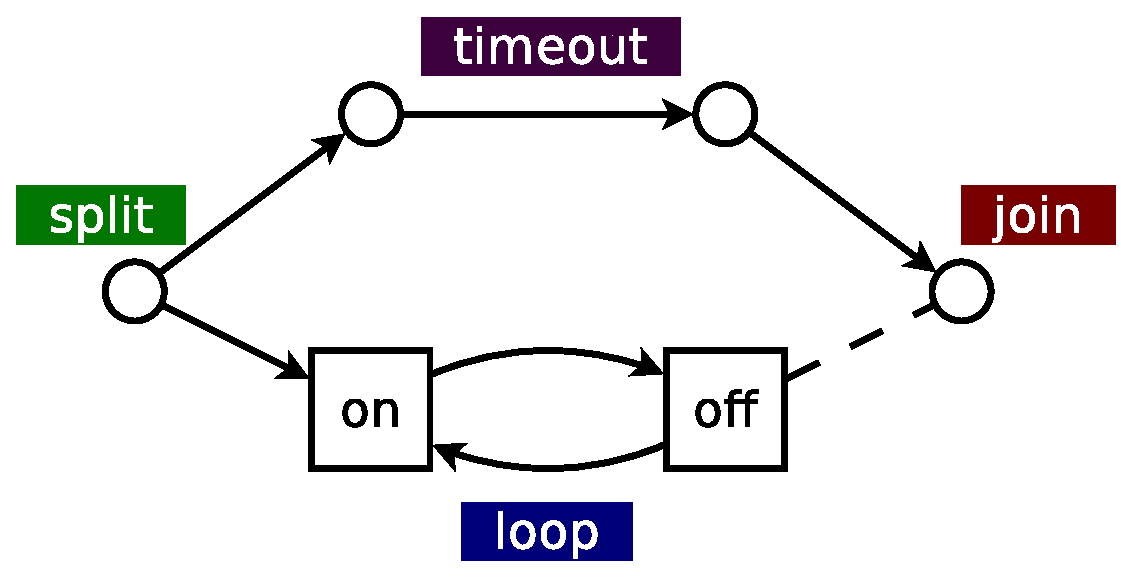
\includegraphics[width=\textwidth]{dia}
\end{minipage}
%%
%\hspace{0.0cm}
%%
\rule{14cm}{0.37pt}
\caption{ ``Blinking LED'' in
    nesC,
    Protothreads,
    and \CEU. %\newline
%{\small
%The colors associate chunks of code with respective actions in the diagram.
%}
\label{lst.all}
}
\end{figure*}

Figure~\ref{lst.all} presents the three synchronous programming (sub-)models 
commonly used in WSNs through a simple concurrent application.
It shows the implementations in \emph{nesC}~\cite{wsn.nesc}, 
\emph{Protothreads}~\cite{wsn.protothreads}, and \CEU for an application that 
continuously turns on a LED for 2 seconds and off for 1 second.
After 1 minute of activity, the application turns off the LED and proceeds to 
another activity (marked in the code as \code{<...>}).
The diagram on the bottom-right of Figure~\ref{lst.all} describes the overall 
control behavior for the application.
The sequential programming pattern is represented by the LED alternating between 
the two states, while the parallel pattern is represented by the 1-minute 
timeout.
% that interrupts the blinking LED.

The first implementation, in \emph{nesC}, which represents the 
\emph{event-driven} model, spawns two timers ``in parallel'' at boot time 
(\code{Boot.booted}): one to make the LED blink and another to wait for 1 
minute.
The callback \code{T1.fired} continuously toggles the LED and resets the timer 
according to the state variable \code{on}.
The callback \code{T2.fired} executes only once, canceling the blinking timer, 
and proceeds to \code{<...>}.
Overall, we argue that this implementation has little structure: the blinking 
loop is not explicit, but instead relies on a static state variable and 
multiple invocations of the same callback.
Furthermore, the timeout handler (\code{T2.fired}) requires specific knowledge 
about how to stop the blinking activity, and the programmer must manually 
terminate it (\code{T1.cancel()}).

The second implementation, in \emph{Protothreads}, which represents the 
\emph{multi-threaded} model~\cite{wsn.protothreads,wsn.mantisos}, uses a 
dedicated thread to make the LED blink in a loop.
This brings more structure to the solution.
The main thread also helps a reader to identify the overall sequence of the 
program, which is not easily identifiable in the event-driven implementation 
without tracking the dependencies among callbacks.
However, it still requires bookkeeping for initializing, scheduling and 
rejoining the blinking thread after the timeout (inside the \code{while} 
condition).

% ASYNC MT?

The third implementation, in \CEU, which represents the 
\emph{synchronous-language model}, uses a \code{par/or} construct to run the 
two activities in parallel:
an endless loop to blink the LED, and a single statement that waits for 1 
minute before terminating.
The \code{par/or} stands for \emph{parallel-or} and rejoins automatically when 
any of its trails terminates.
%
We argue that the hierarchical structure of \CEU more closely reflects the 
control diagram and ties the two activities together, implying that
(a) they can only exist together;
(b) they always start together
(c) they always terminate together.
%
Besides the arguably cleaner syntax, the additional control-flow information 
that can be inferred from the program is the base for all features and safety 
guarantees introduced by \CEU.

% TODO
%The challenge is how to provide a design that embraces/xxx safety/determinism, 
%specially considering pointers

The use of timers in the example of Figure~\ref{lst.all} illustrates 
\emph{split-phase} control operations typically found in WSN 
applications~\cite{wsn.tos}, which require a pair of request and answer 
to/from the underlying system (e.g. \code{T1.start} and \code{T1.fired}).
%
As other examples, requesting sensor readings and forwarding radio packets also 
require split-phase operations and would be programmed similarly to timers in 
each of the three models of Figure~\ref{lst.all}.


\chapter{The design of C\'eu}
    \label{sec.ceu}
    %\begin{documment}

\begin{figure}[t]
\begin{lstlisting}%[backgroundcolor=\color{white}]

// DECLARATIONS
input <type> <id>;      // external event
event <type> <id>;      // internal event
var   <type> <id>;      // variable

// EVENT HANDLING
await <id>;             // awaits event
emit  <id>;             // emits  event

// COMPOUND STATEMENTS
<...> ; <...> ;         // sequence
if <...> then <...>     // conditional
         else <...> end
loop do <...> end       // repetition
    break               //   (escape loop)
finalize <...>          // finalization
    with <...> end

// PARALLEL COMPOSITIONS
par/and do <...>        // rejoins on termination of both sides
      with <...> end
par/or do  <...>        // rejoins on termination of any side
      with <...> end
par do <...>            // never rejoins
  with <...> end

// C INTEGRATION
_f();                   // C call (prefix `_')
native do <...> end     // block of native code
pure <id>;              // pure annotation
safe <id> with <id>;    // safe annotation
\end{lstlisting}
\rule{14cm}{0.37pt}
\caption{ Syntax of \CEU.\newline
{\small %\textmd{
}%}
\label{lst.syntax}
}
\end{figure}

\CEU is a concurrent language in which multiple lines of execution---known as 
\emph{trails}---continuously react to input events from the environment.
Waiting for an event halts the running trail until that event occurs.
The environment broadcasts an occurring event to all active trails, which share 
a single global time reference (the event itself).
%
%\section{Parallel syntactic compositions}
%\label{sec.ceu.par}
%
The fundamental distinction between \CEU and prevailing multi-threaded designs 
is the way threads are combined in programs.
\CEU provides Esterel-like syntactic hierarchical compositions, while most 
multi-threaded systems typically only support top-level definitions for 
threads.
Figure~\ref{lst.syntax} shows a compact reference of \CEU, which helps to 
follow the examples in this chapter.
%\CEU distinguishes itself from Esterel by its tight integration with $C$ and 
%support for shared memory, which also demands an effective safety analysis 
%permeating (and affecting) all language features.

We start the chapter with the fundamental design decisions behind \CEU's 
execution model, namely the uniqueness of external events and deterministic 
scheduler (Section~\ref{sec.ceu.det}).
Then, we discuss how they enable safe concurrency support for shared memory and 
$C$ calls (Sections~\ref{sec.ceu.shared}~and~\ref{sec.ceu.c}).
%
%We follow with discussion about a key characteristic of synchronous languages: 
%activities in parallel that support nesting and abortion 
%(Section~\ref{sec.ceu.par}).
%
We further introduce some new programming features that match \CEU's 
synchronous and safety-oriented design:
local scope finalization (Section~\ref{sec.ceu.fins}),
first-class timers (Section~\ref{sec.ceu.wclocks}),
and a stack-based communication mechanism (Section~\ref{sec.ceu.ints}).
%
We finish with a discussion that summarizes the chapter by comparing \CEU with 
Esterel (Section~\ref{sec.ceu.esterel}).

\section{The execution model of C\'eu}
\label{sec.ceu.det}

% TODO: motivate?

\CEU is grounded on a precise definition of time as a discrete sequence of 
external input events:
% \footnote{We use the terms \emph{external input event}, \emph{external event}, 
%and \emph{input event} interchangeably.}
a sequence because only a single input event is handled at a time; discrete 
because reactions to events are guaranteed to execute in bounded time (to be 
discussed further).
The execution model for \CEU programs is as follows:

\begin{enumerate}
\item The program initiates the ``boot reaction'' in a single trail.
\item Active trails execute until they await or terminate.
      This step is named a \emph{reaction chain}, and always runs in bounded 
      time.
\item The program goes idle and the environment takes control.
\item On the occurrence of a new external input event, the environment awakes 
      \emph{all} trails awaiting that event.
      It then goes to step 2.
\end{enumerate}

% TODO
The synchronous execution model of \CEU is based on the hypothesis that 
internal reactions run \emph{infinitely faster} in comparison to the rate of 
external events~\cite{rp.hypothesis}.
Conceptually, a program takes no time on step 2 and is always idle on step 3.
In practice, if a new external input event occurs while a reaction chain is 
running (step 2), it is enqueued to run in the next reaction.
%, because reaction chains must run to completion.
%
% TODO: a similar approach is taken in \cite{...}
%
When multiple trails are active at a time (i.e. awaking on the same event), 
\CEU schedules them in the order they appear in the program text.
This policy is somewhat arbitrary, but provides a priority scheme for trails, 
and also ensures deterministic and reproducible execution for programs, which 
is important for simulation purposes.
A reaction chain may also contain emissions and reactions to internal events, 
which are presented in Section~\ref{sec.ceu.ints}.

\begin{figure}[h]
\begin{lstlisting}[numbers=left,xleftmargin=2em]
input void A, B, C;
par/and do
    // trail 1
    <...>         // <...> represents non-awaiting statements
    await A;
    <...>
with
    // trail 2
    <...>
    await B;
    <...>
with
    // trail 3
    <...>
    await A;
    <...>
    await B;
    par/and do
        // trail 3
        <...>
    with
        // trail 4
        <...>
    end
end
\end{lstlisting}
%
\rule{14cm}{0.37pt}
\caption{ A \CEU program to illustrate the scheduler behavior.
{\small %\textmd{
}%}
\label{lst.reaction}
}
\end{figure}

\begin{figure}[h]
\centering
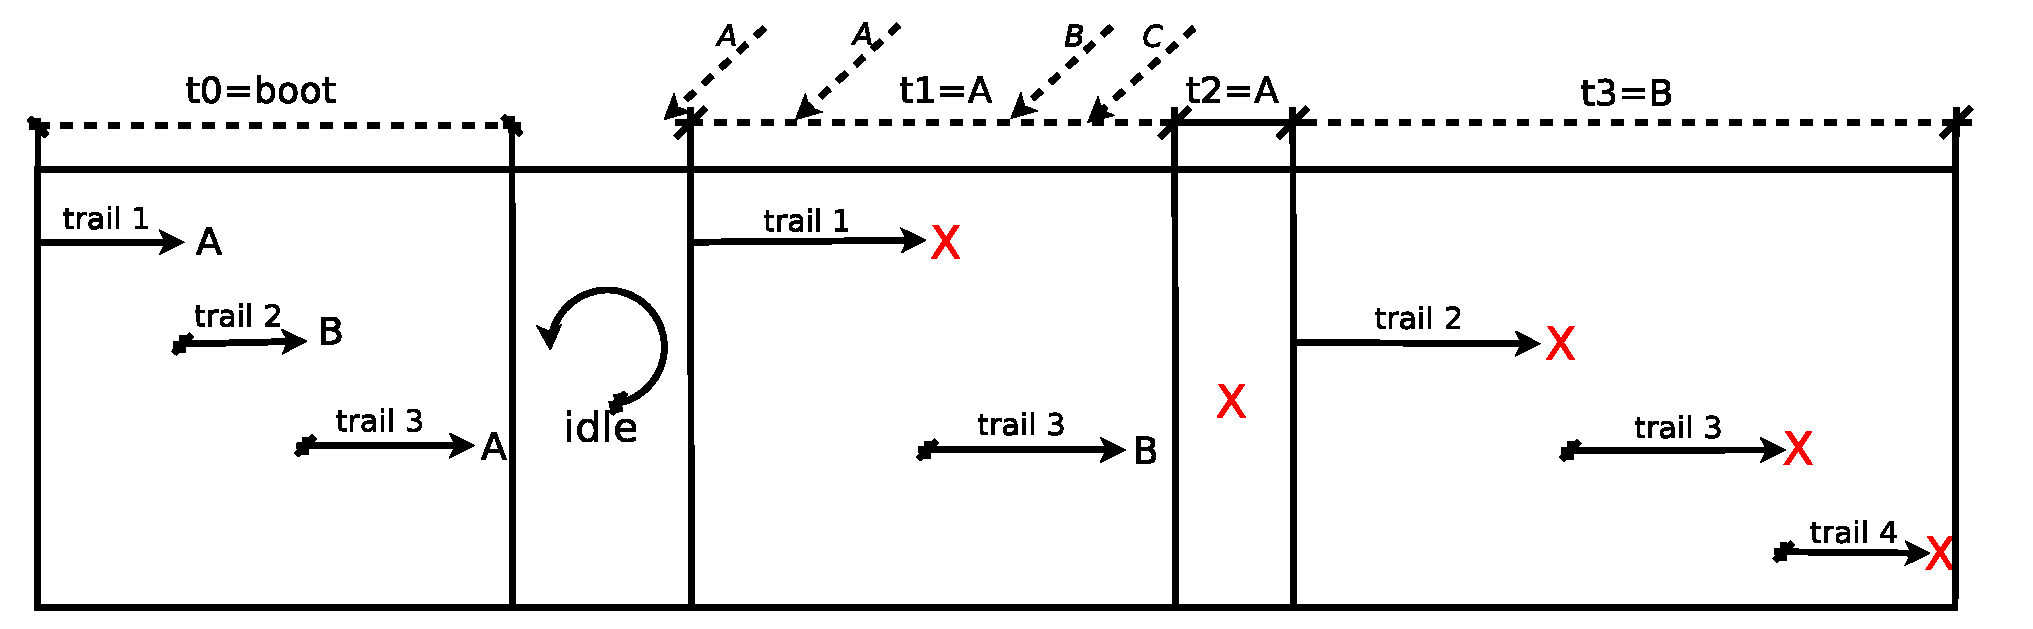
\includegraphics[scale=0.45]{reaction}
\caption{ A sequence of reaction chains for the program in 
Figure~\ref{lst.reaction}.
\label{fig.reaction}
}
\end{figure}

To illustrate the behavior of the scheduler of \CEU, the execution of the 
program in Figure~\ref{lst.reaction} is depicted in the diagram of 
Figure~\ref{fig.reaction}.
%
The program starts in the boot reaction and is split in three trails.
Following the order of declaration, the scheduler first executes \emph{trail~1} 
until it awaits $A$ in line 5;
then \emph{trail~2} executes until it awaits $B$ in line 10;
then \emph{trail~3} is scheduled and also awaits $A$, in line 15.
%
As no other trails are pending, the reaction chain terminates and the scheduler 
remains idle until the occurrence of $A$:
\emph{trail~1} awakes, executes and terminates;
and then \emph{trail 3} executes and waits for $B$ in line 17.
\emph{Trail~2} remains suspended, as it is not awaiting $A$.
%
During this reaction, new instances of events $A$, $B$, and $C$ occur and are 
enqueued to be handled in the reactions that follow.
%
As $A$ happened first, it is used in the next reaction.
However, no trails are awaiting it, so an empty reaction chain takes place.
%
The next reaction dequeues event $B$:
\emph{trail 2} awakes, executes and terminates;
then \emph{trail 3} is split in two and both terminate.
%
The program terminates and does not react to the pending event $C$.
% (the \code{par/and}, to be introduced in the next section, rejoins when its 
%sub-trails terminate).
%
Note that each step in the time line ($t0$, $t1$, etc.) is identified by the 
event it handles.
Inside a reaction, trails only react to that identifying event (or remain 
suspended).

\subsection{Bounded execution}

Reaction chains should run in bounded time to guarantee that programs are 
responsive and can handle upcoming input events from the environment.
Similarly to Esterel~\cite{esterel.ieee91}, \CEU requires that each possible 
path in a loop body contains at least one \code{await} or \code{break} 
statement, thus ensuring that loops never run in unbounded time.
%
Consider the examples that follow:

\nopagebreak
\noindent
\begin{minipage}[t]{0.45\linewidth}
\begin{lstlisting}
loop do
    if <cond> then
        break;
    end
end
\end{lstlisting}
\end{minipage}
%
\begin{minipage}[t]{0.45\linewidth}
\begin{lstlisting}
loop do
    if <cond> then
        break;
    else
        await A;
    end
end
\end{lstlisting}
\end{minipage}

The first example is refused at compile time, because the \code{if} true branch 
may never execute, resulting in a \emph{tight loop} (i.e., an infinite loop 
that does not await).
The second variation is accepted, because for every iteration, the loop either 
breaks or awaits.

Enforcing bounded execution makes \CEU inappropriate for algorithmic-intensive 
applications that require unrestricted loops (e.g., cryptography, image 
processing).
However, \CEU is designed for control-intensive applications and we believe 
this is a reasonable price to pay in order to achieve higher reliability.

\subsection{Parallel compositions and abortion}
\label{sec.ceu.par}

The use of trails in parallel allows that programs wait for multiple events at 
the same time.
Furthermore, trails await without loosing context information, such as locals 
and the program counter, what is a desired behavior in concurrent 
applications.~\cite{sync_async.cooperative}

\CEU supports three kinds of parallel constructs regarding how they rejoin in 
the future:
a \code{par/and} requires that all trails in parallel terminate before 
proceeding to the next statement;
a \code{par/or} requires that any trail in parallel terminates before 
proceeding to the next statement, aborting all awaiting sibling trails;
finally, a \code{par} never rejoins and should be used when trails in parallel 
are supposed to run forever (if they terminate, the scheduler forcedly halts 
them forever).
%
To illustrate how trails rejoin, consider the two variations of the following 
archetype:

\begin{minipage}[t]{0.40\linewidth}
\begin{lstlisting}
loop do
    par/and do
        <...>
    with
        await 100ms;
    end
end
\end{lstlisting}
\end{minipage}
%
\begin{minipage}[t]{0.40\linewidth}
\begin{lstlisting}
loop do
    par/or do
        <...>
    with
        await 100ms;
    end
end
\end{lstlisting}
\end{minipage}

In the \code{par/and} variation, the block marked as \code{<...>} in the first 
trail (which may contain nested compositions with \code{await} statements) is 
repeated every $100$ milliseconds at minimum, as both sides must terminate 
before re-executing the loop.
In the \code{par/or} variation, if the block does not terminate within $100$ 
milliseconds, it is restarted.
These archetypes represent, respectively, the \emph{sampling} and 
\emph{timeout} patterns, which are very common in reactive applications.

The code in Figure~\ref{lst.radio} is extracted from our implementation of the 
\emph{CC2420} radio driver and uses a \code{par/or} to control the start/stop 
behavior of the radio.
The input events \code{CC2420\_START} and \code{CC2420\_STOP} (line 1) 
represent the external interface of the driver with a client application (e.g.  
a protocol).
The driver enters the top-level loop and awaits the starting event (line 3);
once the client application makes a start request, the driver spawns two other 
trails:
one to await the stopping event (line 5),
and another to actually receive radio messages in a loop (collapsed in line 9).
%
As compositions can be nested, the receiving loop can be as complex as needed, 
including other loops and parallel constructs.
However, once the client requests to stop the driver, the trail in line 5 
awakes and terminates, causing the \code{par/or} also terminate and abort the 
receiving loop.
In this case, the top-level loop restarts and waits for the next request to 
start the radio (line 3, again).

\begin{figure}[t]
\begin{lstlisting}[numbers=left,xleftmargin=2em]
input void CC2420_START, CC2420_STOP;
loop do
    await CC2420_START;
    par/or do
        await CC2420_STOP;
    with
        // loop with other nested trails
        // to receive radio packets
        <...>
    end
end
\end{lstlisting}
\rule{14cm}{0.37pt}
\caption{ Start/stop behavior for the radio driver.\newline
{\small %\textmd{
The occurrence of \code{CC2420\_STOP} (line 5) seamlessly aborts the receiving 
loop (collapsed in line 9) and resets the driver to wait for the next 
\code{CC2420\_START} (line 3).
}%}
\label{lst.radio}
}
\end{figure}

The \code{par/or} construct of \CEU is regarded as an \emph{orthogonal 
preemption primitive}~\cite{esterel.preemption} because the two sides in the 
composition need not to be tweaked with synchronization primitives or state 
variables in
order to affect each other.
In contrast, it is known that traditional (asynchronous) multi-threaded 
languages cannot express thread abortion 
safely~\cite{esterel.preemption,sync_async.threadsstop}.

\subsection{Reasoning about concurrency}

The blinking LED of Figure~\ref{lst.all} in \CEU illustrates how synchronous 
parallel constructs lead to a simpler reasoning about concurrency aspects in 
comparison to the other implementations.
As reaction times are assumed to be instantaneous, the blinking loop takes 
exactly 3 seconds (i.e., $2s+1s$).
Hence, after 20 iterations, the accumulated time becomes 60 seconds and the 
loop terminates concurrently with the 1-minute timeout in parallel.
Given that the loop appears first in the code, the scheduler will restart it 
and turn on the LED for the last time.
Then, the 1-minute timeout is scheduled, aborts the whole \code{par/or}, and 
turns off the LED.
%
This reasoning is actually reproducible in practice, and the LED will light on 
exactly 21 times for every single execution of this program.
First-class timers are discussed in more detail in 
Section~\ref{sec.ceu.wclocks}.
%
Note that this static control inference is impossible in asynchronous 
languages, given that internal reactions take an unpredictable time (as 
illustrated in Figure~\ref{lst.related.leds}).
Even in the other implementations of Figure~\ref{lst.all}, this control 
inference cannot be easily extracted, specially considering the presence of two 
different timers.

The behavior for the LED timeout just described denotes a \emph{weak abortion}, 
because the blinking trail had the chance to execute for the last time.
By inverting the two trails, the \code{par/or} would terminate immediately, and 
the blinking trail would not execute, denoting a \emph{strong 
abortion}~\cite{esterel.preemption}.
%
\CEU not only provides means to choose between weak and strong abortion, but 
also detects the two conflicting possibilities and issues a warning at compile 
time (to be discussed in Section~\ref{sec.ceu.shared}).

% TODO: pause

\section{Shared-memory concurrency}
\label{sec.ceu.shared}

WSN applications make extensive use of shared memory, such as for handling 
memory pools, message queues, routing tables, etc.
Hence, an important goal of \CEU is to ensure a reliable execution for 
concurrent programs that share memory.
%
Concurrency in \CEU is characterized when two or more trail segments in 
parallel execute during the same reaction chain.
A trail segment is a sequence of statements followed by an \code{await} (or 
termination).

In the first code fragment that follows, the two assignments to \code{x} run 
concurrently, because both trail segments are spawned during the same reaction 
chain.
However, in the second code fragment, the assignments to \code{y} are never 
concurrent, because \code{A} and \code{B} are different external events and the 
respective segments can never execute during the same reaction chain:

\nopagebreak
\noindent
\begin{minipage}[t]{0.45\linewidth}
\begin{lstlisting}
var int x=1;
par/and do
    x = x + 1;
with
    x = x * 2;
end
\end{lstlisting}
\end{minipage}
%
\begin{minipage}[t]{0.45\linewidth}
\begin{lstlisting}
input void A, B;
var int y=0;
par/and do
    await A;
    y = y + 1;
with
    await B;
    y = y * 2;
end
\end{lstlisting}
\end{minipage}

Note that although the variable \code{x} is accessed concurrently in the first 
example, the assignments are both atomic and deterministic: the final value of 
\code{x} is always $4$ (i.e. {\small$(1+1)*2)$}).
%
Remember from Section~\ref{sec.ceu.det} that trails are scheduled in the order 
they appear and run to completion (i.e., until they await or 
terminate).
%
However, programs with concurrent accesses to shared memory are suspicious, 
because an apparently innocuous reordering of trails modifies the semantics of 
the program; for instance, the previous example would yield $3$ with the trails 
reordered, i.e., {\small$(1*2+1)$}.

%Moreover, \CEU also supports pointers, which are required for low-level 
%manipulation (e.g., accessing buffers from device drivers).

We developed a compile-time temporal analysis for \CEU in order to detect 
concurrent accesses to shared variables, as follows:
\emph{if a variable is written in a trail segment, then a concurrent trail 
segment cannot read or write to that variable, nor dereference a pointer of 
that variable type.}
An analogous policy is applied for pointers \emph{vs} variables and pointers 
\emph{vs} pointers.
The algorithm for the analysis holds the set of all events in preceding 
\code{await} statements for each variable access.
Then, the sets for all accesses in parallel trails are compared to assert that 
no events are shared among them.
Otherwise the compiler warns about the suspicious accesses.

Consider the three examples in Figure~\ref{lst.det}.
The first code is detected as suspicious, because the assignments to \code{x} 
and \code{p} (lines 11 and 14) may be concurrent in a reaction to \code{A} 
(lines 6 and 13);
%
In the second code, although two of the assignments to \code{y} occur in 
reactions to \code{A} (lines 4-5 and 10-11), they are not in parallel trails 
and, hence, are safe.
Note that the assignment in reaction to \code{B} (line 8) is safe given that 
reactions to different events cannot overlap (due to the single-event rule).
%
The third code illustrates a false positive in our algorithm: the assignments 
to \code{z} in parallel can only occur in different reactions to \code{A} 
(lines 5 and 9), as the second assignment awaits two occurrences of \code{A}, 
while the first trail assigns and terminates in the first occurrence.

\begin{figure}[t]
\begin{minipage}[t]{0.39\linewidth}
\begin{lstlisting}[numbers=left,xleftmargin=2em]
input void A;
var int x;
var int* p;
par/or do
  loop do
    await A;
    if <cnd> then
      break;
    end
  end
  x = 1;
with
  await A;
  *p = 2;
end

\end{lstlisting}
\end{minipage}
%
%
\begin{minipage}[t]{0.33\linewidth}
\begin{lstlisting}
input void A, B;
var int y;
par/or do
  await A;
  y = 1;
with
  await B;
  y = 2;
end
await A;
y = 3;

\end{lstlisting}
\end{minipage}
%
%
\begin{minipage}[t]{0.25\linewidth}
\begin{lstlisting}
input void A;
var int z;
par/and do
  await A;
  z = 1;
with
  await A;
  await A;
  z = 2;
end
\end{lstlisting}
\end{minipage}
%
\rule{14cm}{0.37pt}
\caption{ Automatic detection for concurrent accesses to shared memory. \newline
{\small %\textmd{
The first example is suspicious because \code{x} and \code{p} can be accessed 
concurrently (lines 11 and 14).
The second example is safe because accesses to \code{y} can only occur in 
sequence.
The third example illustrates a false positive in our algorithm.
}%}
\label{lst.det}
}
\end{figure}

Conflicting weak and strong abortions, as introduced in 
Section~\ref{sec.ceu.det}, are also detected with the proposed algorithm.
Besides accesses to variables, the algorithm also keeps track of trail 
terminations inside a \code{par/or}, issuing a warning when they can occur 
concurrently.
This way, the programmer can be aware about the conflict existence and choose
between weak or strong abortion.

The proposed static analysis is only possible due to the uniqueness of external 
events within reactions and support for syntactic compositions, which provide 
precise information about the flow of trails (i.e., which run in parallel and 
which are guaranteed to be in sequence).
Such precious information cannot be inferred when the program relies on state 
variables to handle control, as typically occurs in event-driven systems.

We also implemented an alternative algorithm that converts a \CEU program into 
a deterministic finite automata.
The resulting DFA represents all possible points a program can reach during 
runtime and, hence, eliminates all false positives.
However, the algorithm is exponential and may be impractical in some 
situations.
%
That being said, the simpler static analysis does not detect false positives in 
any of the
implementations to be presented in Section~\ref{sec.eval} and executes in 
negligible time, suggesting that the algorithm is practical.

\section{Integration with $C$}
\label{sec.ceu.c}

Most existing operating systems and libraries for WSNs are based on $C$, given 
its omnipresence and level of portability across embedded platforms.
Therefore, it is fundamental that programs in \CEU have access to all 
functionality the underlying platform already provides.

In \CEU, any identifier prefixed with an underscore is repassed \emph{as is} to 
the $C$ compiler that generates the final binary.
Therefore, access to $C$ is seamless and, more importantly, easily trackable.
%
\CEU also supports \emph{native~blocks} to define new symbols in $C$, as 
Figure~\ref{lst.c} illustrates.
Code inside ``\code{native~do~...~end}'' is also repassed to the $C$ compiler 
for the final generation phase.
%Only global definitions are allowed inside $C$ blocks.
As \CEU{} mimics the type system of $C$, values can be easily passed back and 
forth between the languages.

% TODO: real example?
\begin{figure}[t]
\begin{lstlisting}[numbers=left,xleftmargin=2em]
native do
    #include <assert.h>
    int I = 0;
    int inc (int i) {
        return I+i;
    }
end
native _assert(), _inc(), _I;
_assert(_inc(_I));
\end{lstlisting}
%
\rule{14cm}{0.37pt}
\caption{ A \CEU program with embedded $C$ definitions.
{\small %\textmd{
The globals \code{I} and \code{inc} are defined in the \code{native} block 
(lines 3 and 4), and are imported by \CEU in line 8.
$C$ symbols must be prefixed with an underline to be used in \CEU (line 9).
}%}
\label{lst.c}
}
\end{figure}

$C$ calls are fully integrated with the static analysis presented in
Section~\ref{sec.ceu.shared} and cannot appear in concurrent trails segments, 
because \CEU has no knowledge about their side effects.
Also, passing variables as parameters counts as read accesses to them, while 
passing pointers counts as write accesses to those types (because functions may 
dereference and assign to them).
%
This policy increases considerably the number of false positives in the 
analysis, given that many functions can actually be safely called concurrently.
Therefore, \CEU supports explicit syntactic annotations to relax the policy.
They are illustrated in Figure~\ref{lst.annotations}, and are described as 
follows:

\begin{itemize}
\item The \code{pure} modifier declares a $C$ function that does not cause side 
      effects, allowing it to be called concurrently with any other function in 
the program.
\item The \code{safe} modifier declares a pair of variables or functions that 
      do not affect each other, allowing them to be used concurrently.
\end{itemize}

%The following code illustrates \CEU annotations:
%
% TODO: exs from ports

\begin{figure}[t]
\begin{lstlisting}[numbers=left,xleftmargin=2em]
pure  _abs();               // side-effect free
safe _Leds_led0Toggle with  // 'led0' vs 'led1' is safe
     _Leds_led1Toggle;
var int* buf1, buf2;        // point to different buffers
safe buf1 with buf2;        // 'buf1' vs 'buf2' is safe
\end{lstlisting}
\caption{ Annotations for $C$ functions. \newline
{\small %\textmd{
Function \code{abs} is side-effect free and can be concurrent with any other 
function.
The functions \code{\_Leds\_led0Toggle} and \code{\_Leds\_led1Toggle} can 
execute concurrently.
The variables \code{buf1} and \code{buf2} can be accessed concurrently 
(annotations are also applied to variables).
}%}
\label{lst.annotations}
}
\end{figure}

\begin{comment}
TODO

Annotations are typically write-once declarations (when integrating a $C$ 
service for the first time) to be included in actual applications.
Note that the example in Figure~\ref{lst.blink} should include the annotation 
for \code{\_Leds\_led0Toggle} and \code{\_Leds\_led1Toggle} above to be 
compiled correctly.
\end{comment}

\CEU does not extend the bounded execution analysis to $C$ function calls. 
% which are left as responsibility for the programmer.
% TODO: other languages dont as well
On the one hand, $C$ calls must be carefully analyzed in order to keep programs 
responsive.
On the other hand, they also provide means to circumvent the rigor of \CEU in a 
well-marked way (the special underscore syntax).
%
\begin{comment}
This approach is also adopted by Esterel, which supports the \code{call} 
primitive to execute code assumed to be instantaneous in the host 
language~\cite{esterel.primer}.
In \CEU, we take a step further and statically detects when such calls may 
execute concurrently, as discussed in the next section.
\end{comment}
%
Evidently, programs should only resort to $C$ for simple operations that can be 
assumed to be instantaneous, such as non-blocking I/O and \code{struct} 
accessors, but never for control purposes.
% (e.g. interrupt handling).

\section{Local scopes and finalization}
\label{sec.ceu.fins}

\begin{comment}
Furthermore, system-level development typically involves accesses to the 
underlying platform through $C$ system calls that hold pointers for some time
(e.g. transmission of a message buffer).
Hence, if a local variable goes out of scope and its reference has been 
exposed, a system-level activity may end up with a dangling pointer (i.e. a 
pointer to a freed memory).
\end{comment}

Local declarations for variables bring definitions closer to their use in 
programs, increasing the readability and containment of code.
Another benefit, specially in the context of WSNs, is that blocks in sequence 
can share the same memory space, as they can never be active at the same time.
%
The syntactic compositions of trails allows the \CEU compiler to statically 
allocate and optimize memory usage:
%, as also proposed in other systems~\cite{wsn.osm,wsn.ocram}:
memory for trails in parallel must coexist;
trails that follow rejoin points reuse all memory.

However, the unrestricted use of locals may introduce subtle bugs when dealing 
with pointers and $C$ functions interfacing with device drivers.
Given that hardware components outlive the scope of any local variable, a 
pointer passed as parameter to a system call may be held by a device driver
for longer than the scope of the referred variable, leading to a dangling 
pointer.

The code snippet in Figure~\ref{lst.local} was extracted from our 
implementation of the CTP collection protocol~\cite{wsn.teps}.
The protocol contains a complex control hierarchy in which the trail that sends 
beacon frames (lines 11-16) may be aborted from multiple \code{par/or} trails 
(all collapsed in lines 3, 5, and 9).
%
Now, consider the following behavior:
The sending trail awakes from a beacon timer (line 11).
The local message buffer (line 12) is prepared and passed to the radio driver 
(line 13-15).
While waiting for an acknowledgment from the driver (line 16), the protocol 
receives a request to stop (line 3) that aborts the sending trail and makes the 
local buffer go out of scope.
As the radio driver runs asynchronously and still holds the reference to the 
message (passed in line 15), it may manipulate the dangling pointer.
%
\begin{comment}
The message buffer is declared only where it is required (line 12, in the 6th 
depth-level of the program), but its reference is manipulated by two $TinyOS$ 
global functions:
\code{AMSend\_getPayload} (line 13), which returns the data region of the 
message to be sent; %prepared (collapsed in line 14);
and \code{AMSend\_send} (line 15), which requests the operating system to 
actually send the message.
As the radio driver runs asynchronously and holds the reference to the message 
until it is completely transmitted, the sending trail may be aborted in the 
meantime, resulting in a dangling pointer in the program.
\end{comment}
%
A possible solution is to cancel the message send in all trails that can abort 
the sending trail (through a call to \code{AMSend\_cancel}).
However, this would require expanding the scope of the message buffer, adding a 
state variable to keep track of the sending status, and duplicating the code, 
increasing considerably the complexity of the application.

\begin{figure}[t]
\begin{lstlisting}[numbers=left,xleftmargin=2em]
<...>
par/or do
   <...>         // stops the protocol or radio
with
   <...>         // neighbour request
with
   loop do
      par/or do
         <...>   // resends request
      with
         await (dt) ms; // beacon timer expired
         var _message_t msg;
         payload = _AMSend_getPayload(&msg,...);
         <prepare the message>
         _AMSend_send(..., &msg, ...);
         await CTP_ROUTE_RADIO_SENDDONE;
      end
   end
end
\end{lstlisting}
%
\rule{14cm}{0.37pt}
\caption{ Unsafe use of local references. \newline
{\small %\textmd{
The period in which the radio driver manipulates the reference to \code{msg} 
passed by \code{\_AMSend\_send} (line 15) may outlive the lifetime of the 
variable scope, leading to an undefined behavior in the program.
}%}
\label{lst.local}
}
\end{figure}

\CEU provides a safer and simpler solution with the following rule:
\emph{$C$ calls that receive pointers require a finalization block to safely 
handle referred variables going out of scope}.
This rule prevents the previous example to compile, forcing the relevant parts 
to be be rewritten as

\noindent
\begin{minipage}{\linewidth}
\begin{lstlisting}[numbers=left,xleftmargin=2em]
native nohold _AMSend_getPayload();
    <...>
        var _message_t msg;
        <...>
        finalize
            _AMSend_send(..., &msg, ...);
        with
            _AMSend_cancel(&msg);
        end
   <...>
\end{lstlisting}
\end{minipage}

First, the \code{nohold} annotation informs the compiler that the referred $C$ 
function does not require finalization code because it does not hold references 
(line 1).
Second, the \code{finalize} construct (lines 5-9) automatically executes the 
\code{with} clause (line 8) when the variable passed as parameter in the 
\code{finalize} clause (line 6) goes out of scope.
Therefore, regardless of how the sending trail is aborted, the finalization 
code politely requests the OS to cancel the ongoing send operation (line 8).

All network protocols that we implemented in \CEU use this finalization 
mechanism for message sends.
%
We looked through the TinyOS code base and realized that among the $349$ calls 
to the \code{AMSend.send} interface, only $49$ have corresponding 
\code{AMSend.cancel} calls.
We verified that many of these \emph{sends} should indeed have matching 
\emph{cancels} because the component provides a \emph{stop} interface for 
clients.
In \emph{nesC}, because message buffers are usually globals, a send that is not 
properly canceled typically results in an extra packet transmission that 
wastes battery.
However, in the presence of dynamic message pools, a misbehaving program can 
change the contents of a (not freed) message that is actually about to be 
transmitted, leading to a subtle bug that is hard to track.

%find . -name "*.nc" | xargs egrep -R "\.send\(|\.send \(" | grep -v command | 
%wc
%=> 349

%find . -name "*.nc" | xargs egrep -R "\.cancel\(|\.cancel \(" | grep -v command | wc
%=> 49

The finalization mechanism is fundamental to preserve the orthogonality of the
\code{par/or} construct, i.e., an aborted trail does not require clean up code 
outside it.

\begin{comment}
% TODO: expand
During the porting process, we identified two potentially harmful system calls 
that require

The send/cancel pattern occurs in all ported applications that use the radio 
for communication evaluated in Section~\ref{sec.eval}.

 that  two dangerous

given that the porting process was straightforward, we believe that the 
\emph{nesC} implementation is free of such ...
However, .
performance degradation
another endorsement

- exception srp queue
we know exactly the place where it occurs
nesC no

* cancel
* timers
* locals

%TODO: LOCALS AND PAR COMPOSITIONS ARE A PERFECT MATCH

As a final consideration, we propose to extend the idea of compositions by 
combining different \emph{applications} together.
In the context of WSNs, it is usually difficult to physically recover motes in 
a deployed network, and by combining multiple applications in a single image, 
we can switch their execution remotely via radio.
The following archetype illustrates this idea:

\nopagebreak
\noindent
\begin{minipage}{\linewidth}
\begin{lstlisting}[numbers=left,xleftmargin=2em]
input int SWITCH;
var int app = 1;
loop do
   par/or do
      app = await SWITCH;
   with
      if app == 1 then
         <CODE for APP1>
      else/if app == 2 then
         <CODE for APP2>
      end
      await FOREVER;
   end
end
\end{lstlisting}
\end{minipage}

The input event \code{SWITCH} (line 1) is used to request application switches 
remotely.%
\footnote{ We are assuming the existence of an hypothetical high-level event 
\code{Switch} that abstracts the radio protocol for requests to change the 
current running application. }
Initially, the code behaves as application $1$ (lines 7-9), but is also waiting 
for a \code{Switch} request in parallel (line 5).
Whenever a new request occurs, the \code{par/or} terminates, aborts the running 
application, and restarts as the requested application.
The \code{await Forever} statement (line 13) ensures that a terminating 
application does not restart itself.

The same idea can be used to \emph{reboot} a mote remotely, in the case of a 
strange behavior in an application.
\end{comment}

\section{First-class timers}
\label{sec.ceu.wclocks}

% TODO: ana

Activities that involve reactions to \emph{wall-clock time}%
\footnote{
By wall-clock time we mean the passage of time from the real world, measured in 
hours, minutes, etc.
}
appear in typical patterns of WSNs, such as timeouts and sensor sampling.
However, support for wall-clock time is somewhat low-level in existing 
languages, usually through timer callbacks or sleep blocking calls.
%
In any concrete system implementation, however, a requested timeout does not 
expire precisely with zero-delay, a fact that is usually ignored in the 
development process.
We define the difference between the requested timeout and the actual expiring 
time as the \emph{residual delta time (delta)}.
Without explicit manipulation, the recurrent use of timed activities in 
sequence (or in a loop) may accumulate a considerable amount of deltas that can 
lead to incorrect behavior in programs.

The \code{await} statement of \CEU supports wall-clock time and handles deltas 
automatically, resulting in more robust applications.
As an example, consider the following program:

\nopagebreak
\noindent
\begin{minipage}{\linewidth}
\begin{lstlisting}[xleftmargin=2em]
var int v;
await 10ms;
v = 1;
await 1ms;
v = 2;
\end{lstlisting}
\end{minipage}

Suppose that after the first \code{await} request, the underlying system gets 
busy and takes 15ms to check for expiring awaits.
The \CEU scheduler will notice that the \code{await 10ms} has not only already 
expired, but delayed with \code{delta=5ms}.
Then, the awaiting trail awakes, sets \code{v=1}, and invokes \code{await 1ms}.
As the current delta is higher than the requested timeout (i.e. $5ms > 1ms$), 
the trail is rescheduled for execution, now with \code{delta=4ms}.

\CEU also takes into account the fact that time is a physical quantity that can 
be added and compared.
For instance, for the program that follows, although the scheduler cannot 
guarantee that the first trail terminates exactly in 11ms, it can at least 
ensure that the program always terminates with \code{v=1}:

\nopagebreak
\noindent
%\begin{figure}[t]
%\rule{14cm}{0.37pt}
\begin{minipage}{\linewidth}
\begin{lstlisting}[xleftmargin=2em]
par/or do
    await 10ms;
    <...>         // any non-awaiting sequence
    await  1ms;
    v = 1;
with
    await 12ms;
    v = 2;
end
\end{lstlisting}
\end{minipage}
%\rule{14cm}{0.37pt}
%\caption{ The first trail always terminates the program.
%\label{lst.time}
%}
%\end{figure}

Remember that any non-awaiting sequence is considered to take no time in the 
synchronous model.
Hence, the first trail is guaranteed to terminate before the second trail, 
because $10+1 < 12$.
A similar program in a language without first-class support for timers, would 
depend on the execution timings for the code marked as \code{<...>}, making the 
reasoning about the execution behavior more difficult.
%
The importance of synchronized timers becomes more evident in the presence of 
loops, like in the introductory example of Figure~\ref{lst.all} in which the 
first trail is guaranteed to execute exactly 21 times before being aborted by 
the timer in the second trail.

Note that in extreme scenarios, small timers in sequence (or in a loop) may 
never ``catch up'' with the external clock, resulting in a \emph{delta} that
increases indefinitely.
%There is nothing \CEU can do about that, as it is do
To deal with such cases, the current \emph{delta} is always returned from an 
\code{await} and can be used in programs:

\begin{lstlisting}
loop do
    var int late = await 1ms;
    if late < 1000 then
        <...>   // normal behavior
    else
        <...>   // abnormal behavior
    end
end
\end{lstlisting}

% TODO: uses in ports
% trickle?

%\newpage
\section{Internal events}
\label{sec.ceu.ints}

% TODO: ana

\CEU provides internal events as a signaling mechanism among parallel trails:
a trail that invokes \code{await~e} can be awoken in the future by a trail that 
invokes \code{emit~e}.

In contrast with external events, which are handled in a queue, internal events 
follow a stack policy.
In practical terms, this means that a trail that emits an internal event pauses 
until all trails awaiting that event completely react to it, continuing to 
execute afterwards.
%
Another difference to external events is that internal events occur in the same 
reaction chain they are emitted, i.e., an \code{emit} instantaneously matches 
and awakes all corresponding \code{await} statements that were invoked in 
\emph{previous reaction chains}%
\footnote{In order to ensure bounded reactions, an \code{await} statement 
cannot awake in the same reaction chain it is invoked.}.

The stacked execution for internal events introduces support for a restricted 
form of subroutines that cannot express recursive definitions (either directly 
or indirectly), resulting in bounded memory and execution time.
% that preclude stack overflows.
% TODO: exec bounded
% TODO: why?
%
Figure~\ref{lst.func} shows how the dissemination trail from our implementation 
of the DRIP protocol simulates a function and can be invoked from different 
parts of the program (lines 16-19), just like a subroutine.
The \code{await send} (line 17) represents the function entry point, which is 
surrounded by a \code{loop} so that it can be invoked repeatedly.
The DRIP protocol distinguishes data and metadata packets and disseminates one 
or the other based on a request parameter.
For instance, when the trickle timer expires (line 8), the program invokes 
\code{emit~send=>1} (line 9), which awakes the dissemination trail (line 17) 
and starts sending a metadata packet (collapsed in line 18).
Note that if the trail is already sending a packet, then the \code{emit} will 
not match the \code{await} and will have no effect (the \emph{nesC} 
implementation uses an explicit state variable to attain this same behavior).

% TODO: missed sends / non reentrancy

\begin{figure}[t]
%\rule{14cm}{0.37pt}
\begin{lstlisting}[numbers=left,xleftmargin=2em]
event int send;
par do
    <...>
        await DRIP_KEY;
        emit send => 0;     // broadcast data
with
    <...>
        await DRIP_TRICKLE;
        emit send => 1;     // broadcast meta
with
    <...>
        var _message_t* msg = await DRIP_DATA_RECEIVE;
        <...>
        emit send => 0;     // broadcast data
with
    loop do
        var int isMeta = await send;
        <...>   // send data or metadata (contains awaits)
    end
end
\end{lstlisting}
\rule{14cm}{0.37pt}
\caption{ A loop that awaits an internal event can emulate a subroutine.  \newline
{\small %\textmd{
The \code{send} ``subroutine'' (lines 16-19) is invoked from three different 
parts of the program (lines 5, 9, and 14).
}%}
\label{lst.func}
}
\end{figure}

This form of subroutines has some significant limitations:

\begin{description}
\item[\emph{Single instance}:] Calls to a running subroutine have no effect.
As noted in the example of Figure~\ref{lst.func}, a subroutine that awaits on 
its body may miss further calls to it (in some cases this behavior is actually 
desired).
%
\item[\emph{Single calling}:] Further calls to a subroutine in a reaction chain 
also have no effect.
Even if a subroutine terminates within a reaction chain (i.e. reaches the 
\code{await} again), other \code{emit} invocations are ignored until the next 
reaction chain.
Remember that $await$ statements must be awaiting before the reaction chain 
starts to be awoken and that \code{emit} statements are immediately broadcast 
(i.e., they are not buffered).
%
\item[\emph{No recursion}:] Recursive calls to a subroutine also have no 
effect.
For the same reason of the \emph{single instance} property, a trail cannot be 
awaiting itself while running and the recursive call is ignored.
%
\item[\emph{No concurrency}:] If two trails in parallel try to call the same 
subroutine, the static analysis warns about non-determinism.
Even if the warning is ignored, the call from the first trail takes effect 
(based on deterministic scheduling), while the second call fails on the 
\emph{single call} property.
\end{description}

\vspace{5pt}
\CEU provides no support for standard functions for a number of reasons:
\begin{itemize}
\item The interaction with other \CEU control primitives is not obvious (e.g., 
executing an $await$ or a $par/or$ inside a function).
\item They would still be restricted in some ways given the embedded context 
(e.g. no recursion or closures).
\item Programs can always recur to $C$ when absolutely necessary.
%\item A dedicated primitive would behave just as described, being a matter of 
%syntactic sugar.
\end{itemize}

Regardless of the limitations, this form of subroutines is widely adopted in 
\CEU programs, given that they were designed to work with the other control 
mechanisms.
Keep in mind that the typical reactive organization of programs (awaiting an 
external stimulus, reacting to it, and going back to awaiting) does not demand 
recursive subroutines.

Internal events also provide means for describing more elaborate control 
structures, such as \emph{exceptions}.
The code in Figure~\ref{lst.exception} handles incoming packets for the CC2420 
radio driver in a loop.
After awaking from a new packet notification (line 4), the program enters in a 
sequence to read the bytes from the hardware buffer (lines 8-16).
If any anomaly is found on the received data, the program invokes 
\code{emit~next} to discard the current packet (lines 10 and 14).
Given the execution semantics of internal events, the \code{emit} continuation 
is stacked and awakes the trail in line 6, which terminates and aborts the 
whole \code{par/or} in which the emitting trail is paused.
Therefore, the continuation for the \code{emit} never resumes, and the loop 
restarts to await a next packet.

% TODO: resumable

\begin{figure}[t]
%\rule{14cm}{0.37pt}
\begin{lstlisting}[numbers=left,xleftmargin=2em]
<...>
event void next;
loop do
    await CC_RECV_FIFOP;
    par/or do
        await next;
    with
        <...>   // (contains awaits)
        if rxFrameLength > _MAC_PACKET_SIZE then
            emit next;  // packet is too large
        end
        <...>   // (contains awaits)
        if rxFrameLength == 0 then
            emit next;  // packet is empty
        end
        <...>   // (contains awaits)
    end
end
\end{lstlisting}
\rule{14cm}{0.37pt}
\caption{ Exception handling in \CEU. \newline
{\small
The \code{emit}'s in lines 10 and 14 raise an exception to be caught by the 
\code{await} in line 6.
The \code{emit} continuations are discarded given that the surrounding 
\code{par/or} is aborted.
}
\label{lst.exception}
}
\end{figure}

\section{Differences to Esterel}
\label{sec.ceu.esterel}

A primary goal of \CEU is to support reliable shared-memory and $C$ concurrency 
on top of a deterministic scheduler and effective safety analysis
(Sections~\ref{sec.ceu.det},~\ref{sec.ceu.shared}~and~\ref{sec.ceu.c}).
%
Esterel, however, does not support shared-memory concurrency because \emph{``if 
a variable is written by some thread, then it can neither be read nor be 
written by concurrent threads''}~\cite{esterel.primer}.
%
Furthermore, Esterel is deterministic only with respect to reactive control, 
i.e., \emph{``the same sequence of inputs always produces the same sequence of 
outputs''}~\cite{esterel.primer}.
However, the order of execution for side-effect operations within a reaction is 
non-deterministic: \emph{``if there is no control dependency and no signal 
dependency, as in "\code{call f1() || call f2()}", the order is unspecified and 
it would be an error to rely on it''}~\cite{esterel.primer}.
%
%In \CEU, when multiple trails are active at a time, as in
%``\code{par/and~do~\_f1()~with~\_f2()~end}'', they are scheduled in the order 
%they appear in the program text (i.e. \code{\_f1} executes first).

In Esterel, an external reaction can carry simultaneous signals, while in \CEU, 
a single event defines a reaction.
%Figure~\ref{fig.reactions} illustrates this difference.
%TODO
%
The notion of time in Esterel is similar to that of digital circuits, in which 
multiple wires (signals) can be queried for their status (\emph{present} or 
\emph{absent}) on each clock tick.
%
\CEU more closely reflects event-driven programming, in which occurring events 
are sequentially and uninterruptedly handled by the program.
%
This design decision is fundamental for the temporal analysis of 
Section~\ref{sec.ceu.shared}.%, which assumes that

Esterel makes no semantic distinctions between internal and external signals, 
both having only the notion of presence or absence during the entire 
reaction~\cite{esterel.preemption}.
%
In \CEU, however, internal and external events behave differently:
%
\begin{itemize}
\item External events can be emitted only by the environment, while internal 
events only by the program.
\item A single external event can be active at a time, while multiple internal 
events can coexist within a reaction.
\item External events are handled in a queue, while internal events follow a 
stacked execution policy.
\end{itemize}
%
In particular, the stack-based execution policy for internal events in \CEU 
enables a limited but safe form of subroutines and an exception-handling 
mechanism, as discussed in Section~\ref{sec.ceu.ints}.

Apart from these fundamental differences to Esterel, \CEU introduces 
first-class timers with a convenient syntax and predictable behavior 
(Section~\ref{sec.ceu.wclocks}), and also finalization blocks to safely handle 
memory going out of scope (Section~\ref{sec.ceu.fins}).

% TODO
%\section{Limitations}
%\section{External API}


\chapter{Demo applications}
    \label{sec.demos}
    In this chapter, we present two demos that explore the high-level and safety 
capabilities of \CEU described in the previous chapter.
%
Our goal is to present full commented applications that help understanding and 
getting familiar with the language.
%
The applications are somewhat simple (70 and 170 lines), but complete enough to 
expose the programming techniques promoted by \CEU.

The first demo targets commercially available 16-bit WSN nodes, such as 
\emph{micaZ} and \emph{telosb}%
\footnote{\url{http://www.xbow.com}}.
The second demo uses the Arduino open-source platform%
\footnote{\url{http://arduino.cc}}, in order to experiment with custom
third-party hardware.
Both platforms have low processing power and memory capacity (16Mhz CPU, 32Kb 
Flash, and 4Kb SRAM), showing that \CEU is applicable to highly constrained 
platforms.

\section{WSN ring}
\label{sec:demos:ring}

In the first demo, we implement a fixed-ring topology with $N$ motes placed 
side-by-side which should all follow the same behavior: receive a message with 
an integer counter, show it on the LEDs, wait for $1$ second, increment the 
counter, and forward it to the mote on its right.
%Note that using fixed topologies and running the same application in all motes 
%are common practices in the context of WSNs.
%
Because the topology constitutes a ring, the counter will be incremented 
forever while traversing the motes.
%
If a mote does not receive a message within $5$ seconds, it should blink the 
red LED every $500$ milliseconds until a new message is received.
%In a ring topology, communications traverse all motes, and the network goes 
%down with a failure in a single mote, making tests much easier.
%
The mote with \emph{id=0} is responsible for initiating the process at boot 
time and recovering the ring from failures.
On perceiving a failure, it should wait for $10$ seconds before retrying the 
communication.

\begin{figure}[ht]
\begin{lstlisting}[numbers=left,xleftmargin=2em]
loop do
    var _message_t* msg = await RADIO_RECEIVE;
    var int* cnt = _Radio_getPayload(msg);
    _Leds_set(*cnt);
    await 1s;
    *cnt = *cnt + 1;
    finalize
        _Radio_send((_NODE_ID+1)%N, msg);
    with
        _Radio_cancel(msg);
    end
    await RADIO_SENDDONE;
end
\end{lstlisting}
\rule{14cm}{0.37pt}
\caption{ Communicating trail for the WSN ring.%\newline
{\small %\textmd{
%The code is a simple loop that does not handle failures.
}%}
\label{lst.ring.1}
}
\end{figure}

Figure~\ref{lst.ring.1} implements the communicating trail, which continuously 
receives and forwards the messages.
%
The code is an endless loop that first awaits a radio message (line 2), gets a 
pointer to its data buffer (line 3), shows the received counter on the LEDs 
(line 4), and then awaits $1$s (line 5) before incrementing the counter in the 
message (line 6) and forwarding it to the next mote (line 7-12).

The program uses several services provided by the underlying operating system 
(\cite{wsn.tos}), which are all non-blocking $C$ functions for LEDs and radio 
manipulation.

The finalization block (lines 7-11) ensures that regardless of how the 
communicating trail is composed with the rest of the application (and 
eventually aborted by it), the \code{msg} buffer will be safely released while 
waiting for a \code{RADIO\_SENDDONE} acknowledge from the radio driver.

Because this code does not handle failures, it is straight to the point and 
easy to follow.
Actually, this is the final code for this task, as error handling is placed in 
a parallel trail.

\begin{comment}
Note that the program accesses the message buffer multiple times in reaction to 
events.
However, given that the \code{await} primitive provides sequential flow across 
reactions to events, every access to the buffer in the code is undoubtedly 
deterministic.
In typical event-driven systems~\cite{wsn.nesc}, the accesses would be split in 
multiple callbacks, requiring a thoughtful reasoning about concurrency issues.
\end{comment}

\begin{figure}[ht]
\begin{lstlisting}[numbers=left,xleftmargin=2em]
par do
    <...> // COMMUNICATING TRAIL (previous code)
with
    loop do
        par/or do
            await RADIO_RECEIVE;
        with
            await 5s;
            par do
                loop do
                    emit retry; // only captured by mote 0
                    await 10s;
                end
            with
                _Leds_set(0);   // clear LEDs
                loop do
                    _Leds_led0Toggle();
                    await 500ms;
                end
            end
        end
    end
end
\end{lstlisting}
\rule{14cm}{0.37pt}
\caption{ Monitoring trail for the WSN ring.%\newline
{\small %\textmd{
%The code is a simple loop that does not handle failures.
}%}
\label{lst.ring.2}
}
\end{figure}

To handle failures, we define in Figure~\ref{lst.ring.2} a monitoring trail 
(lines 4-22) in parallel with the communicating trail.
%
Lines 8 to 20 describe the network-down behavior.
After $5$ seconds of inactivity are detected in the sub-trails in parallel 
(lines 6 and 8), two new activities run in parallel: one that retries 
communication every $10$ seconds by signaling the internal event \code{retry} 
(lines 8-11); and another that blinks the red LED every $500$ milliseconds 
(lines 13-17).

The trick to restore the normal behavior of the network is to await event 
\code{RADIO\_RECEIVE} (line 6) in the \code{par/or} (line 5) with the 
network-down behavior to abort it whenever a new message is received.
By surrounding everything with a \code{loop} (line 4), we ensure that the error 
detection is continuous.

\begin{figure}[ht]
\begin{lstlisting}[numbers=left,xleftmargin=2em]
par do
    <...> // COMMUNICATING TRAIL
with
    <...> // MONITORING TRAIL
with
    if _NODE_ID == 0 then
        loop do
            var _message_t msg;
            var int* cnt = _Radio_getPayload(&msg);
            *cnt = 1;
            finalize
                _Radio_send(1, &msg);
            with
                _Radio_cancel(&msg);
            end
            await retry;
        end
    else
        await FOREVER;
    end
end
\end{lstlisting}
\rule{14cm}{0.37pt}
\caption{ Retrying trail for the WSN ring.%\newline
{\small %\textmd{
%The code is a simple loop that does not handle failures.
}%}
\label{lst.ring.3}
}
\end{figure}

Finally, we implement in Figure~\ref{lst.ring.3} the initiating/retrying 
process that sends the first message from mote with \emph{id=0}.
Again, we place the code (lines 6-20) in parallel with the other activities.
%
As this process is only handled by the mote with $id=0$, we start by checking 
it (line 6).
If this is not the case, we simply await forever on this trail (line 19).
Otherwise, the \code{loop} (lines 7-17) sends the first message as soon as the 
mote is turned on (line 12).
It then waits for a \code{retry} emit (line 16) to loop and resend the initial 
message.
Remind that event \code{retry} is emitted on network-down every $10$ seconds 
(line 10 of previous code).

The static analysis of \CEU correctly warns about concurrent calls to 
\code{\_Radio\_send} (line 12) \emph{vs.} \code{\_Leds\_set} and 
\code{\_Leds\_led0Toggle} (lines 13,15 of previous code), which all execute 
after the program detects 5 seconds of inactivity (line 6 of previous code).
However, because these functions affect different devices (i.e. radio 
\emph{vs.} LEDs), they can be safely executed concurrently.
The following annotation (to be included in the program) states that these 
specific functions can be called concurrently with deterministic behavior, 
allowing the program to be compiled without warnings:

\begin{lstlisting}
  safe _Radio_send with
       _Leds_set, _Leds_led0Toggle;
\end{lstlisting}

This example shows how complementary activities in an application can be 
written in separate and need not to be mixed in the code.
In particular, error handling (monitoring trail) need not to interfere with 
regular behavior (communicating trail), and can even be incorporated later.
To ensure that parallel activities exhibit deterministic behavior, the \CEU 
compiler rejects harmful concurrent $C$ calls by default.

\begin{figure}[ht]
\begin{lstlisting}[numbers=left,xleftmargin=2em]
input int SWITCH;
var int cur_app = 1;
loop do
    par/or do
        cur_app = await SWITCH;
    with
        if cur_app == 1 then
            <...>  // CODE for APP1
        end
        if cur_app == 2 then
            <...>  // CODE for APP2
        end
        await FOREVER;
    end
end
\end{lstlisting}
\rule{14cm}{0.37pt}
\caption{ Retrying trail for the WSN ring.%\newline
{\small %\textmd{
%The code is a simple loop that does not handle failures.
}%}
\label{lst.app}
}
\end{figure}

As a final consideration, we can extend the idea of compositions by combining 
different \emph{applications} together.
In the context of WSNs, it is usually difficult to physically recover motes in 
a deployed network, and by combining multiple applications in a single image, 
we can switch their execution remotely via radio.
%
The archetype in Figure~\ref{lst.app} illustrates this idea.
%
The input event \code{SWITCH} (line 1) is used to request application switches 
remotely.%
\footnote{ We are assuming the existence of an hypothetical high-level event 
\code{SWITCH} that abstracts the radio protocol for requests to change the 
current running application. }
Initially, the code behaves as application $1$ (lines 7-9), but is also waiting 
for a \code{SWITCH} request in parallel (line 5).
Whenever a new request occurs, the \code{par/or} terminates, aborts the running 
application, and restarts as the requested application.
The \code{await FOREVER} statement (line 13) ensures that a terminating 
application does not reach the end of the \code{par/or} and restarts itself.

The same idea can be used to \emph{reboot} a mote remotely, in the case of a 
strange behavior in an application.

\section{Spaceship game}

In the next demo, a spaceship game, we control a ship that moves through space 
and has to avoid collisions with meteors until it reaches the finish line.
%
Although this application is not networked, it is still embedded and reactive, 
using timers, buttons, and an LCD with real-time feedback.
%
We use an Arduino connected to a third-party two-row LCD display with two 
buttons to exhibit and control the spaceship.
%
Figure~\ref{fig:ship} shows the picture of a running quest.

\begin{figure}[t]
\centering
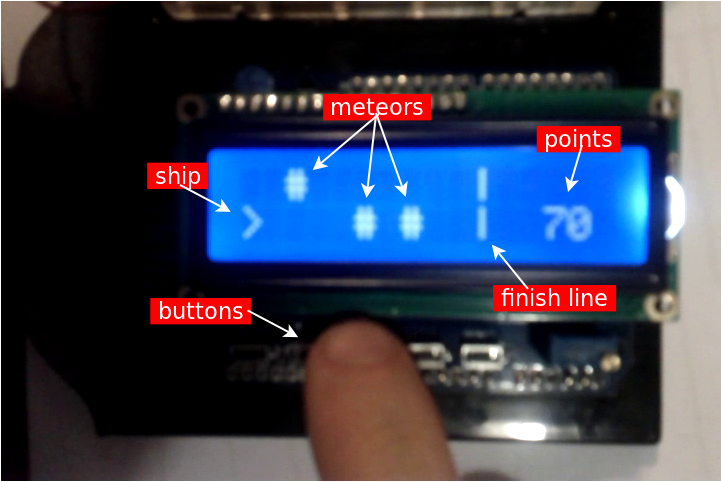
\includegraphics[scale=0.30]{ship.png}
\caption{ The ``spaceship'' game
\label{fig:ship}
}
\end{figure}

\begin{figure}[ht]
\begin{lstlisting}[numbers=left,xleftmargin=2em]
var int dt;       // inverse of game speed
var int points;   // number of steps alive
var int win = 0;  // starting the game

loop do
    <...> // CODE 1: set game attributes

    _map_generate();
    _redraw(x, y, points);
    await KEY;  // starting key

    <...> // CODE 2: the central loop

    <...> // CODE 3: game over
end
\end{lstlisting}
\rule{14cm}{0.37pt}
\caption{ Outermost loop for the game.
{\small %\textmd{
%The code is a simple loop that does not handle failures.
}%}
\label{lst.ship.1}
}
\end{figure}

We describe the behavior of the game, along with its implementation, following 
a top-down approach.
The outermost loop of the game, in Figure~\ref{lst.ship.1}, is constituted of 
\code{CODE~1}, which sets the game attributes such as globals \code{code} and 
\code{dt}; \code{CODE~2} with the central game loop; and \code{CODE~3} with the 
``game over'' animation.
%
Every time the loop is executed, it resets the game attributes (line 5), 
generates a new map (line 7), redraws it on screen (line 8), and waits for a 
starting key (line 9).
Then, the program executes the main logic of the game (line 11), until the 
spaceship reaches the finish line or collides with a meteor.
Depending on the result held in \code{win}, the ``game over'' code (line 13) 
may display an animation before restarting the game.

\begin{figure}[ht]
\begin{lstlisting}[numbers=left,xleftmargin=2em]
    // CODE 1: set game attributes
    var int y = 0;          // ship coordinates
    var int x = 0;          //  restart every phase

    if not win then
        dt     = 500;
        points = 0;
    else
        if dt > 100 then
            dt = dt - 50;
        end
    end
\end{lstlisting}
\rule{14cm}{0.37pt}
\caption{ Sets the game attributes.
{\small %\textmd{
%The code is a simple loop that does not handle failures.
}%}
\label{lst.ship.2}
}
\end{figure}

The game attributes (\code{CODE 1} in Figure~\ref{lst.ship.2}) change depending 
on the result of the previous iteration of the outermost loop.
%
For the first game execution and whenever the spaceship collides with a meteor, 
variable \code{win} is false, hence, the attributes are reset to their initial 
values (lines 6-7)
Otherwise, if the player reached the finish line, then the game gets faster, 
keeping the current points (lines 9-11).

\begin{figure}[ht]
\begin{lstlisting}[numbers=left,xleftmargin=2em]
    // CODE 2: the central loop
    par/or do
        loop do
            await (dt)ms;
            x = x + 1;
            _redraw(x, y, points);

            if _MAP[y][x] == '#' then
                win = 0;  // a collision
                break;
            end

            if x == _FINISH then
                win = 1;  // finish line
                break;
            end

            points = points + 1;
        end
    with
        loop do
            var int key = await KEY;
            if key == _KEY_UP then
                y = 0;
            end
            if key == _KEY_DOWN then
                y = 1;
            end
        end
    end;
\end{lstlisting}
\caption{ The game central loop.
{\small %\textmd{
%The code is a simple loop that does not handle failures.
}%}
\label{lst.ship.3}
}
\end{figure}

The central loop of the game (\code{CODE 2}  in Figure~\ref{lst.ship.3}) moves 
the spaceship as time elapses and checks whether the spaceship reaches the 
finish line or collides with a meteor.
%
The code is actually split in two loops in parallel: one that runs the game 
steps (lines 3-19), and the other that handles input from the player to move 
the spaceship (lines 21-29).
Note that we want the spaceship to move only during the game action, this is 
why we did not place the input handling in parallel with the whole application.

The game steps run periodically, depending on the current speed of the game 
(line 4).
For each loop iteration, \code{x} is incremented and the current state is 
redrawn on screen (lines 5-6).
Then, the spaceship is checked for collision with meteors (lines 8-11), and 
also with the finish line (lines 13-16).
In either of the cases, the central loop terminates with \code{win} set to the 
proper value, also canceling the input handling activity.
The points are incremented before each iteration of the loop (line 18).

To handle input events, we wait for key presses in another loop (line 22) and 
change the spaceship position accordingly (lines 24, 27).
Note that there are no possible race conditions on variable \code{y} (i.e., 
lines 6,8 \emph{vs.} 24,27) because the two loops in the \code{par/or} 
statement react to different events (i.e., time and key presses).

\begin{figure}[ht]
\begin{lstlisting}[numbers=left,xleftmargin=2em]
    // CODE 3: game over
    par/or do
        await KEY;
    with
        if !win then
            loop do
                await 100ms;
                _lcd.setCursor(0, y);
                _lcd.write('<');
                await 100ms;
                _lcd.setCursor(0, y);
                _lcd.write('>');
            end
        end
    end
\end{lstlisting}
\caption{ The ``game over'' behavior for the game.
{\small %\textmd{
%The code is a simple loop that does not handle failures.
}%}
\label{lst.ship.4}
}
\end{figure}

After escaping the central loop, we run the code of Figure~\ref{lst.ship.4} for 
the ``game over'' behavior, which starts an animation if the spaceship collides 
with a meteor.
%
The animation loop (lines 6-13) continuously displays the spaceship in the two 
directions, suggesting that it has hit a meteor.
The animation is interrupted when the player presses a key (line 3), proceeding 
to the game restart.
Note the use of the \code{\_lcd} object, available in a third-party \emph{C++} 
library shipped with the LCD display, and used unmodified in the example.

This demo makes extensive use of global variables, relying on the
deterministic concurrency analysis guaranteed by the \CEU compiler.
We used a top-down approach to illustrate the hierarchical compositions of 
blocks of code.
For instance, the ``game over'' animation (lines 6-13) is self-contained and 
can be easily adapted to a new behavior without considering the other parts of 
the program.


\chapter{Evaluation}
    \label{sec.eval}
    %\begin{document}

\begin{figure*}[t]
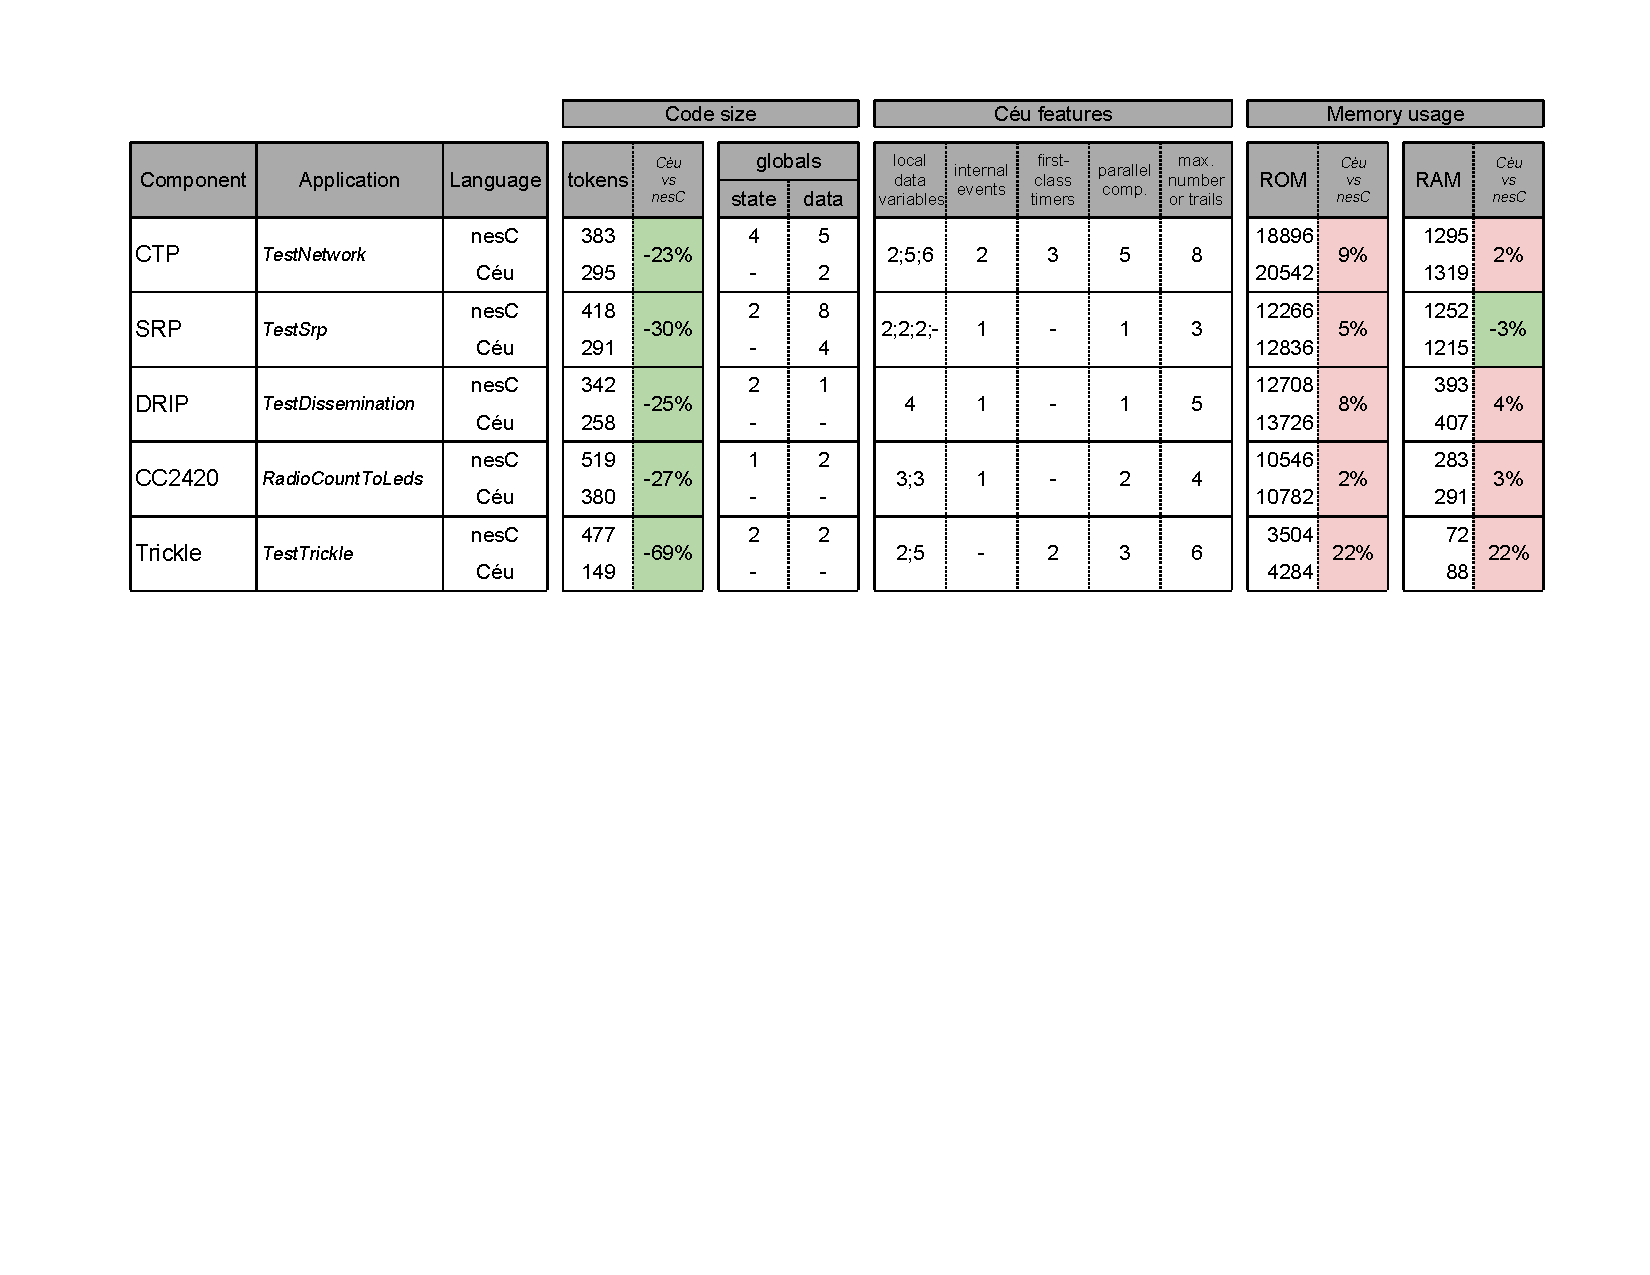
\includegraphics[width=\textwidth]{eval}
%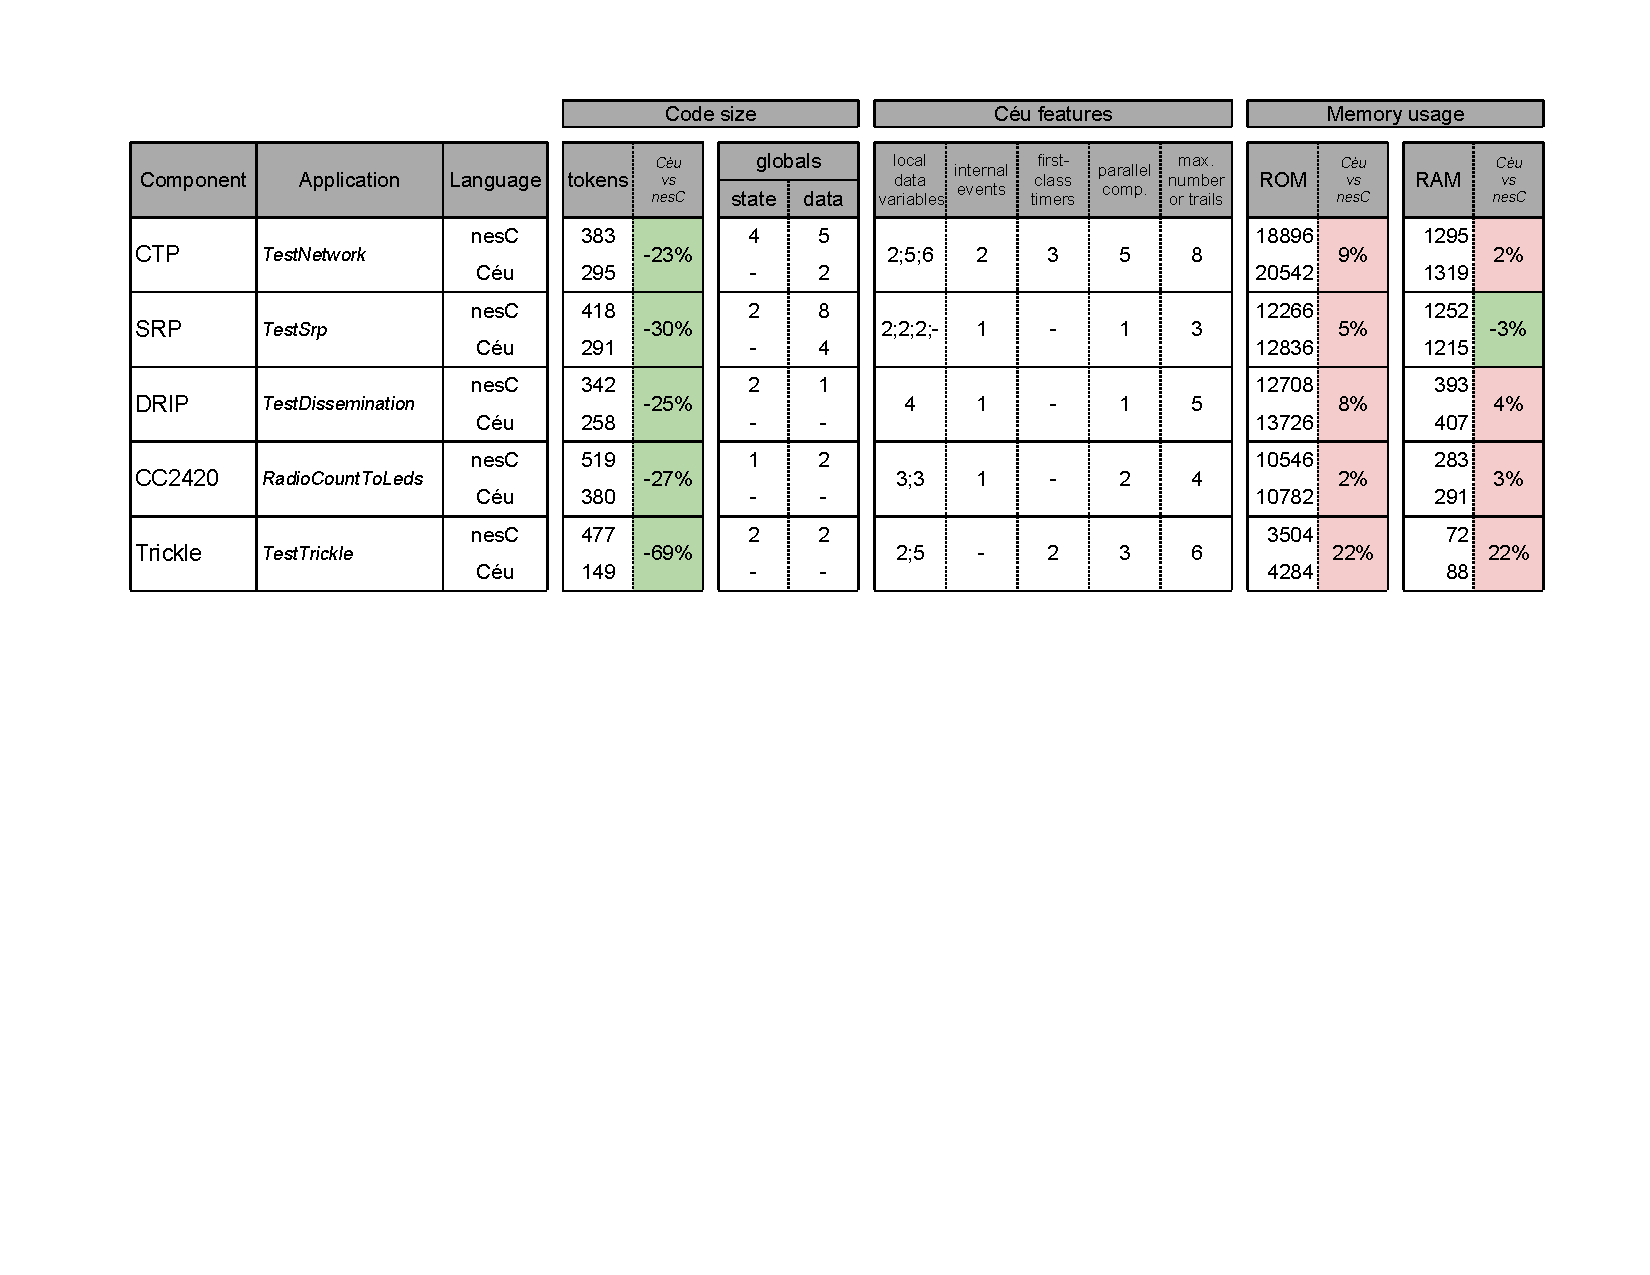
\includegraphics{eval}
\caption{ Comparison between \CEU and \emph{nesC} for the implemented 
applications. \newline
{\small %\textmd{
The column group \emph{Code size} compares the number of language tokens and 
global variables used in the sources;
the group \emph{C\'eu features} shows the number of times each functionality is 
used in each application;
the group \emph{Memory usage} compares ROM and RAM consumption.
}%}
\label{fig.eval}
}
\end{figure*}

In this chapter we present a quantitative evaluation of \CEU.
%
Our assumption is that when considering \CEU for system-level development, 
programmers would face a tradeoff between code simplicity and efficient 
resource usage.
%
For this reason, we evaluate source code size, memory usage, event-handling 
responsiveness, and battery consumption for a number of standardized protocols 
in TinyOS~\cite{wsn.teps}.
%
We use code size as a metric for code simplicity, complemented with a 
qualitative discussion regarding the eradication of explicit state variables 
for control purposes.
%
By responsiveness, we mean how quickly programs react to incoming events (to 
avoid missing them).
%
Memory, responsiveness are important resource-efficiency measures to evaluate 
the negative impact with the adoption of a higher-level language.
%
In particular, responsiveness (instead of total CPU cycles) is a critical 
aspect in reactive systems, specially those with a synchronous execution 
semantics where preemption is forbidden.
%
We also discuss battery consumption when evaluating responsiveness.

Our criteria to choose which language and applications to compare with \CEU are 
based on the following guidelines:
%
\begin{itemize}
\item Compare to a resource-efficient programming language in terms of memory 
and speed.
\item Compare to the best available codebase, with proved stability and 
quality.
\item Compare relevant protocols in the context of WSNs.
\item Compare the control-based aspects of applications, as \CEU is designed 
      for this purpose.
\item Compare the radio behavior, the most critical and battery-drainer 
      component in WSNs.
\end{itemize}
%
Based on these criteria, we chose \emph{nesC} as the language to compare, given 
its resource efficiency and high-quality codebase%
\footnote{TinyOS repository: \url{http://github.com/tinyos/tinyos-release/}}.
%
In addition, \nesc is used as benchmark in many systems related to 
\CEU~\cite{wsn.protothreads,wsn.sol,wsn.ocram,wsn.flowtalk}.
In particular, the work on \emph{Protothreads}~\cite{wsn.protothreads} is a 
strong reference in the WSN community, and we adhere to similar choices in our 
evaluation.
%
All chosen applications are reference implementations of open standards in the 
TinyOS community~\cite{wsn.teps}:
the receiving component of the \emph{CC2420} radio driver;
the \emph{Trickle} timer;
the \emph{SRP} routing protocol;
the \emph{DRIP} dissemination protocol;
and the routing component of the \emph{CTP} collection protocol.
%
They are representative of the realm of system-level development for WSNs, 
which mostly consists of network protocols and low-level system utilities:
%
%Justifying each choice individually,
a radio driver is mandatory in the context of WSNs;
the trickle timer is used as a service by other important
protocols~\cite{wsn.trickle,wsn.ctp};
routing, dissemination, and collection are the most common classes of protocols 
in WSNs.

%TTT drip vs dip
%Although DRIP is simpler than other dissemination alternatives~\cite{wsn.dip, 
%wsn.}, they mostly vary on , and we chose the smallest available 
%implementation in \emph{nesC} of each.
%
%The (e.g. DIP

We took advantage of the component-based model of TinyOS and all of our 
implementations use the same interface provided by the \emph{nesC} counterpart.
This approach has two advantages:
first, we could reuse existing applications in the TinyOS repository to test 
the protocols (e.g. \emph{RadioCountToLeds} or \emph{TestNetwork});
second, sticking to the same interface forced us to retain the original 
architecture and functionality, which also strengths our evaluation.

Figure~\ref{fig.eval} shows the comparison for \emph{Code size} and 
\emph{Memory usage} between the implementations in \emph{nesC} and \CEU.
%
For memory usage, detailed in Section~\ref{sec.eval.resource}, we compare the 
binary code size and required RAM.
%
For code size, detailed in Section~\ref{sec.eval.code}, we compare the number 
of tokens used in the source code.
%The figure also details how many times each relevant feature of \CEU was used 
%in the implementations, helping to identify the patterns that reduce the code 
%size (to be discussed further).
%
For responsiveness, detailed in Section~\ref{sec.eval.radio}, we evaluate the 
capacity to promptly acknowledge radio packet arrivals in the $CC2420$ driver.

\section{Code size}
\label{sec.eval.code}

We use two metrics to compare code complexity between the implementations in 
\CEU and \emph{nesC}: the number of language tokens and global variables used 
in the source code.
%
Similarly to comparisons in related work~\cite{wsn.ocram,wsn.protothreads}, we 
did not consider code shared between the \emph{nesC} and \CEU implementations 
(e.g. predicates, \code{struct} accessors, etc.), as they do not represent 
control functionality and pose no challenges regarding concurrency aspects.

%We chose to use tokens instead of lines of code because code density in \CEU 
%is considerably lower, given that most lines are composed of a single block 
%delimiter from a structural composition.
%
Note that the languages share the core syntax for expressions, calls, and field 
accessors (based on $C$), and we removed all verbose annotations from the 
\emph{nesC} implementations for a fair comparison (e.g. \code{signal}, 
\code{call}, \code{command}, etc.).
%
The column \emph{Code size} in Figure~\ref{fig.eval} shows a considerable 
decrease in the number of tokens for all implementations (around at least 
25\%).

Regarding the metrics for number of globals, we categorized them in 
\emph{state} and \emph{data} variables.

State variables are used as a mechanism to control the application flow (on the 
lack of a better primitive).
Keeping track of them is often regarded as a difficult task, hence, reduction 
of state variables has already been proposed as a metric of code complexity in 
a related work~\cite{wsn.protothreads}.
The implementations in \CEU, not only reduced, but completely eliminated state 
variables, given that all control patterns could be expressed with hierarchical 
compositions of activities assisted by internal-event communication.

Data variables in WSN programs usually hold message buffers and protocol 
parameters (e.g. sequence numbers, timer intervals, etc.).
In event-driven systems, given that stacks are not retained across reactions to 
the environment, all data variables must be global%
\footnote{In the case of \emph{nesC}, we refer to globals as all variables 
defined in the top-level of a component implementation block, which are visible 
to all functions inside it.}.
Although the use of local variables does not imply in reduction of lines of 
code (or tokens), the smallest the scope of a variable, the more readable and 
less susceptible to bugs the program becomes.
%
In the \CEU implementations, most variables could be nested to a deeper scope.
The column \emph{local data variables} in Figure~\ref{fig.eval} shows the depth 
of each new local variable in \CEU that was originally a global in \emph{nesC} 
(e.g. ``2;5;6'' represents globals that became locals inside blocks in the 2nd, 
5th, and 6th depth level).

The columns under \emph{C\'eu features} in Figure~\ref{fig.eval} point out how 
many times each functionality has been used in the implementations in \CEU, 
helping to identify where the reduction in size comes from.
%
As an example, Trickle uses 2 timers and 3 parallel compositions, resulting in 
at most 6 trails active at the same time.
% (a \code{par} may spawn more than 2 trails).
The use of six coexisting trails for such a small application is justified by 
its highly control-intensive nature, and the almost 70\% code reduction 
illustrates the huge gains with \CEU in this context.
% TODO: what about CTP? (roberto)
%
%TODO: CTP c/ select

% TODO: DRIP uses trickle as a service (does not implement it)

\section{Memory usage}
\label{sec.eval.resource}

Memory is a scarce resource in motes and it is important that \CEU does not 
pose significant overheads in comparison to \emph{nesC}.
%
We evaluate ROM and RAM consumption by using available testing applications for 
the protocols in the TinyOS repository.
%They were carefully tweaked to generate a minimal binary that tests only the 
%components of interest.
Then, we compiled each application twice: first with the original component in 
\emph{nesC}, and then with the new component in \CEU.
%
Column \emph{Memory usage} in Figure~\ref{fig.eval} shows the consumption of 
ROM and RAM for the generated applications.
With the exception of the Trickle timer, the results in \CEU are below 10\% in 
ROM and 5\% in RAM, in comparison with the implementations in \emph{nesC}.
%
Our method and results are similar to those for
Protothreads~\cite{wsn.protothreads}, which is an actively supported 
programming system for the Contiki OS~\cite{wsn.contiki}.
% with a simple and lightweight implementation based on a set of C macros.

Note that the results for Trickle illustrate the footprint of the runtime of 
\CEU.
The RAM overhead of 22\% actually corresponds to only 16 bytes: 1 byte for each 
of the maximum 6 concurrent trails, and 10 bytes to handle synchronization 
among timers.
%
As the complexity of the application grows, this basic overhead tends to become 
irrelevant.
%
The SRP implementation shows a decrease in RAM, which comes from the internal 
communication mechanism of \CEU that could eliminate a queue.
%
Note that both TinyOS and \CEU define functions to manipulate queues for timers 
and tasks (or trails).
Hence, as our implementations use components in the two systems, we pay an 
extra overhead in ROM for all applications.

We focused most of the language implementation efforts on RAM optimization, as 
it has been historically considered more scarce than ROM~\cite{wsn.decade}.
Although we have achieved competitive results, we expected more gains with 
memory reuse for blocks with locals in sequence, because it is something that 
cannot be done automatically by the \emph{nesC} compiler.
However, we analyzed each application and it turned out that we had no gains 
\emph{at all} from blocks in sequence.
Our conclusion is that sequential patterns in WSN applications come either from 
split-phase operations, which always require memory to be preserved (between 
the request and the answer);
or from loops, which do reuse all memory, but in the same way that event-driven 
systems do.

\section{Responsiveness}
\label{sec.eval.radio}

A known limitation of languages with synchronous and cooperative execution is 
that they cannot guarantee hard real-time 
deadlines~\cite{wsn.comparison,wsn.tosthreads}.
%
For instance, the rigorous synchronous semantics of \CEU forbids 
non-deterministic preemption to serve high priority trails.
%
Even though \CEU ensures bounded execution for reactions, this guarantee is not 
extended to $C$ function calls, which are usually preferred for executing long 
computations (due to performance and existing code base).
%
%Even though WSN protocols are usually tolerant to faults (given the unreliable 
%link), packet losses affect the network performance and cause motes to spend 
%more battery.
%
The implementation of a radio driver purely in \CEU raises questions
regarding its responsiveness, therefore, we conduct two experiments in this 
section.
% in order to evaluate it.
%
The experiments use the \emph{COOJA} simulator~\cite{wsn.cooja} running images 
compiled to \emph{TelosB} motes.

In the first experiment, we ``stress-test'' the radio driver to compare its 
performance in the \CEU and \emph{nesC} implementations.
We use 10 motes that broadcast 100 consecutive packets of 20 bytes to a mote 
that runs a periodic time-consuming activity.
The receiving handler simply adds the value of each received byte to a global 
counter.
% (we set a single random byte for each packet, so that the sum is always 1).
%
The sending rate of each mote is 200ms (leading to a receiving average of 50 
packets per second considering the 10 motes), and the time-consuming activity 
in the receiving mote runs every 140ms.
%
Note that these numbers are much above typical WSN applications: 10 neighbours 
characterizes a dense topology; 20 bytes plus header data is close to the 
default limit for a TinyOS packet; and 5 messages per second is a high 
frequency on networks that are supposedly idle most of the time.
%
We run the experiment varying the duration of the lengthy activity from 1 to 
128 milliseconds, covering a wide set of applications (summarized in 
Table~\ref{tab.durs}).
%
We assume that the lengthy operation is implemented directly in $C$ and cannot 
be easily split in smaller operations (e.g., recursive 
algorithms~\cite{wsn.comparison,wsn.tosthreads}).
So, we simulated them with simple busy waits that would keep the driver in \CEU 
unresponsive during that period.
%(given the run completion semantics of the language).
%We certified that the operation executed the same number of times in \CEU and 
%\emph{nesC} for all tests in the experiment.

Figure~\ref{fig.radio1} shows the percentage of handled packets in \CEU and 
\emph{nesC} for each duration.
%
Starting from the duration of 6ms for the lengthy operation, the responsiveness 
of \CEU degrades in comparison to \nesc (5\% of packet loss).
%every 140ms, while receiving a new packet every 20ms
%
The \emph{nesC} driver starts to become unresponsive with operations that take 
32ms, which is a similar conclusion taken from TOSThreads experiments with the 
same hardware~\cite{wsn.tosthreads}.
%
\begin{comment}
Our direct interpretation is that the \CEU driver starts to become unresponsive 
when receiving packets every 20ms while executing a periodic operation of 16ms 
(which is keeping the CPU unresponsive 80\% of the time).
The same interpretation can be done for \emph{nesC}, but considering a 64-ms 
operation,
\end{comment}
%
Table~\ref{tab.durs} shows the duration of some lengthy operations specifically 
designed for WSNs found in the literature.
The operations in the group with timings up to $6ms$ could be used with 
real-time responsiveness in \CEU (considering the proposed high-load 
parameters).
%a 5\% decrease in performance in comparison with \emph{nesC}.

\begin{figure}[t]
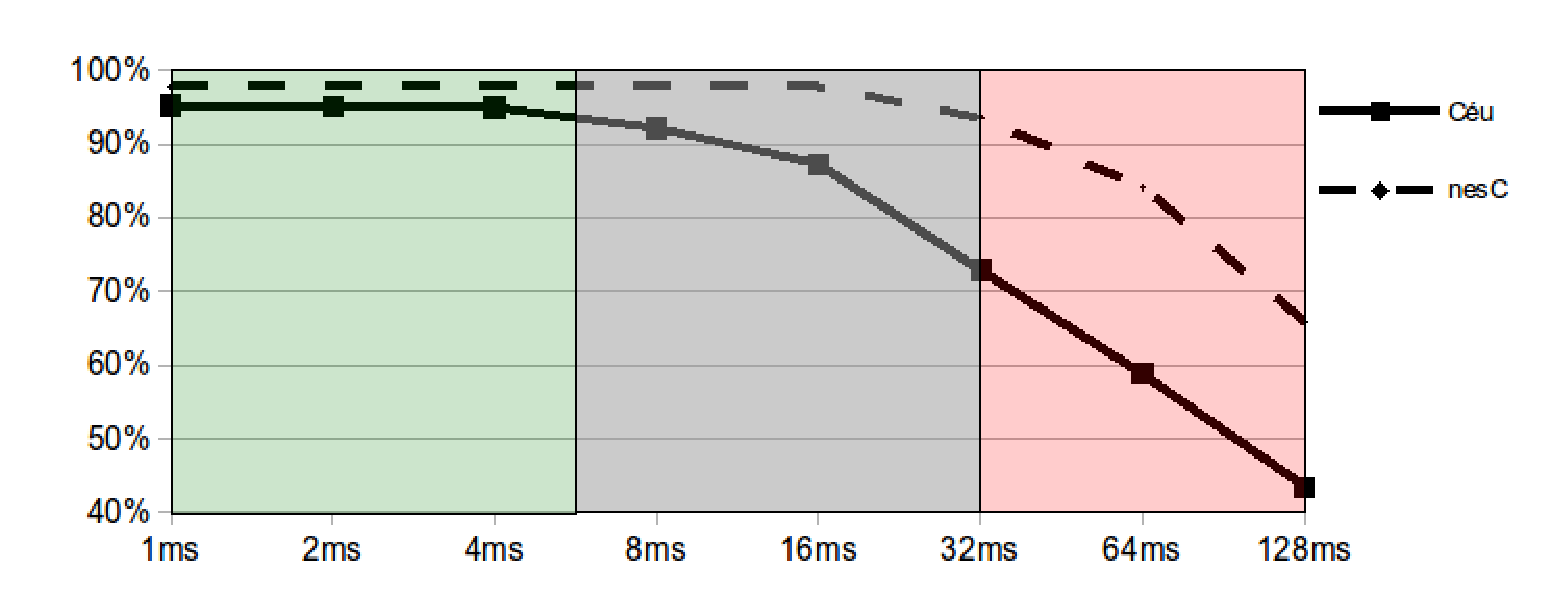
\includegraphics[width=\linewidth,clip=true,trim=5px 0px 5px 0px]{radio1}
%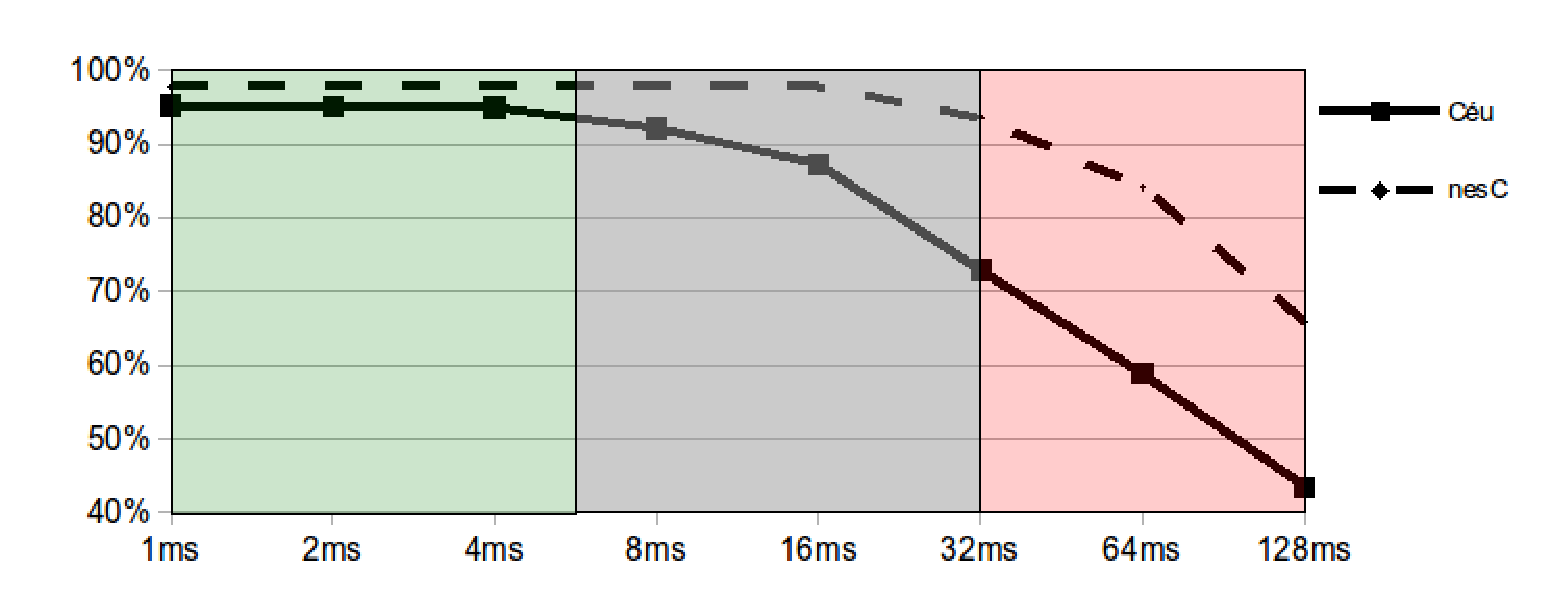
\includegraphics[width=\linewidth,clip=true,trim=35px 0px 10px 0px]{radio1}
%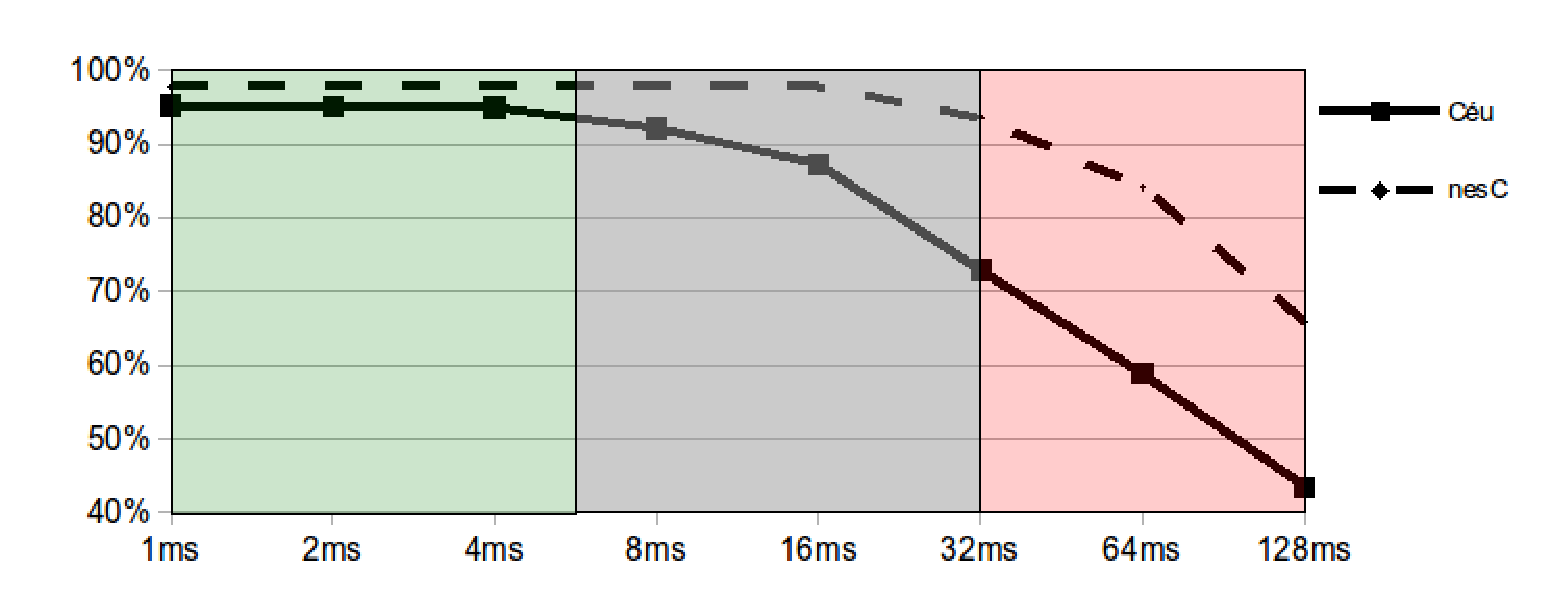
\includegraphics{radio1}
\caption{ Percentage of received packets depending on the duration of the 
lengthy operation.  \newline
{\small %\textmd{
Note the logarithmic scale on the \emph{x}-axis.
The packet arrival frequency is 20ms.
The operation frequency is 140ms.
%Starting from a 16-ms duration, \CEU performs 5\% worse than \emph{nesC}.
In the (left) green area, \CEU performs similarly to \emph{nesC}.
The (middle) gray area represents the region in which \emph{nesC} is still 
responsive.
In the (right) red area, both implementations become unresponsive (i.e. over 
5\% packet losses).
}%}
\label{fig.radio1}
}
\end{figure}

\definecolor{lightgreen}{rgb}{.8,1,0.8}
\definecolor{lightred}{rgb}{1,.8,.8}
\definecolor{darkgray}{rgb}{.66,.66,.66}

\begin{table}[t]
\begin{center}
\begin{tabular}{ | l | r | }
\hline
\rowcolor{darkgray}
    Operation          & Duration  \\ \hline
\hline
\rowcolor{lightgreen}
    Block cypher~\cite{wsn.tinysec,wsn.crypto}  & 1ms           \\ \hline
\rowcolor{lightgreen}
    MD5 hash~\cite{wsn.crypto}                  & 3ms           \\ \hline
\rowcolor{lightgreen}
    Wavelet decomposition~\cite{wsn.wavelet}    & 6ms           \\ \hline
\hline
\rowcolor{lightred}
    SHA-1 hash~\cite{wsn.crypto}                & 8ms           \\ \hline
\rowcolor{lightred}
    RLE compression~\cite{wsn.compression}      & 70ms          \\ \hline
\rowcolor{lightred}
    BWT compression~\cite{wsn.compression}      & 300ms         \\ \hline
\rowcolor{lightred}
    Image processing~\cite{wsn.cyclops}         & 50--1000ms    \\ \hline
\end{tabular}
\caption{Durations for lengthy operations is WSNs. \newline
{\small %\textmd{
\CEU can perform the operations in the green rows in real-time and under high 
loads.
}%}
\label{tab.durs}
}
\end{center}
\end{table}

Although we did not perform specific tests to evaluate CPU usage, the 
experiment suggests that the overhead of \CEU over \emph{nesC} is very low.
%
When the radio driver is the only running activity (column $1ms$, which is the 
same result for an addition test we did for $0ms$), both implementations loose 
packets with a difference under 3 percentage points.
This difference remains the same up to 4-ms activities, hence, the observed 
degradation for longer operations is only due to the lack of preemption, not 
execution speed.
%
Note that for lengthy operations implemented in $C$, there is no runtime 
overhead at all, as the generated code is the same for \CEU and \emph{nesC} 
(i.e. \CEU and \emph{nesC} just call $C$).

In the second experiment, instead of running a long activity in parallel, we 
use a 8-ms operation tied in sequence with every packet arrival to simulate an 
activity such as encryption.
We now run the experiment varying the rate in the 10 sending motes from 600ms 
to 100ms (i.e., 60ms to 10ms receiving rate if we consider the 10 motes).
%
Figure~\ref{fig.radio2} shows the percentage of handled packets in \CEU and 
\emph{nesC} for each rate of message arrival.
%
%The last column shows the theoretical limit of 80ms (i.e., receiving a packet 
%every 8ms and handling it in 8ms).
%
The results show that \CEU is 100\% responsive up to frequency of 33 packets 
per second, while \emph{nesC} up to 50 packets.

\begin{figure}[t]
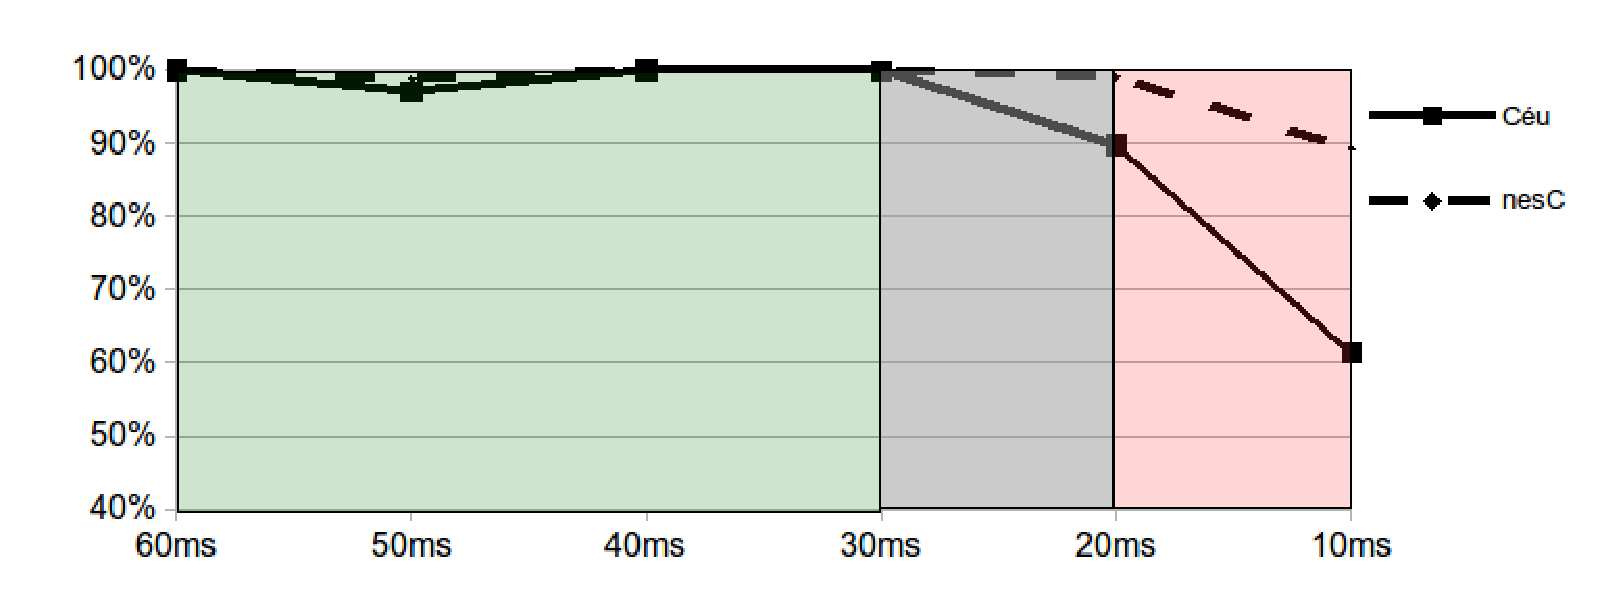
\includegraphics[width=\linewidth,clip=true,trim=5px 0px 5px 0px]{radio2}
%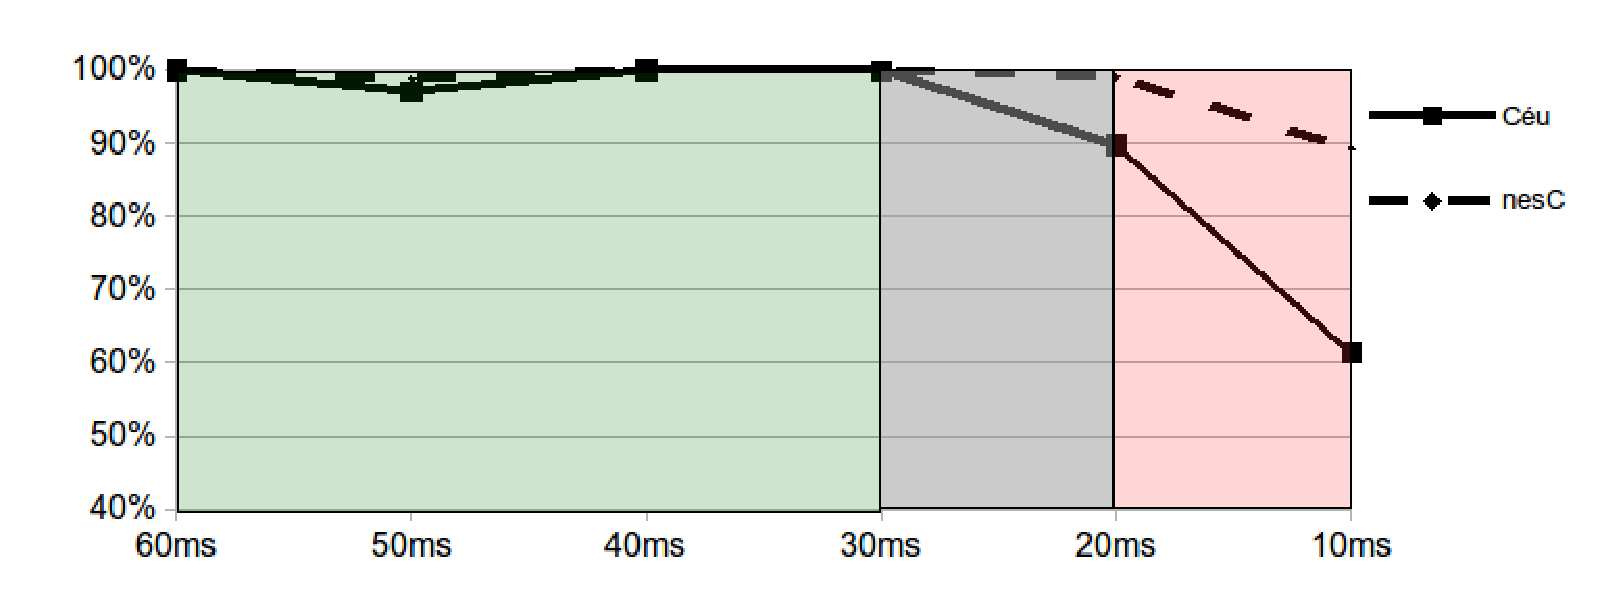
\includegraphics[width=\linewidth,clip=true,trim=35px 0px 10px 0px]{radio2}
\caption{  Percentage of received packets depending on the sending frequency.  
\newline
{\small %\textmd{
Each received packet is tied to a 8-ms operation.
\CEU is 100\% responsive up to a frequency of 30ms per packet.
}%}
\label{fig.radio2}
}
\end{figure}

% TODO: reaction times, measure or cite?

The overall conclusion from the experiments is that the radio driver in \CEU 
performs as well as the original driver in \emph{nesC} under high loads for 
programs with lengthy operations of up to 4ms, which is a reasonable time for 
control execution and simple processing.
%
The range between 6ms and 16ms offers opportunities for performing more complex 
operations, but also requires careful analysis and testing.
%
For instance, the last experiment shows that the \CEU driver can process in 
real time messages arriving every 33ms in sequence with a 8-ms operation.
%
%For operations over 64ms, neither \CEU or \emph{nesC} have real-time 
%responsiveness under high-loads.

Note that our experiments represent a ``stress-test'' scenario that is atypical 
to WSNs.
Protocols commonly use longer intervals between message transmissions together 
with mechanisms to avoid contention, such as randomized 
timers~\cite{wsn.trickle,wsn.ctp}.
Furthermore, WSNs are not subject to strict deadlines, being not classified as 
hard real-time systems~\cite{wsn.decade}.

\section{Battery consumption}
\label{sec.eval.batt}

Battery consumption is critical in WSNs, given that motes usually have no other 
source of energy and, in the case of being deployed in remote locations, cannot 
have the batteries replaced.

In order to evaluate battery consumption in \CEU in comparison to \emph{nesC}, 
we adapted the experiments of Section~\ref{sec.eval.radio}.
%
The parameters were adjusted to make the implementations in the two languages 
behave the same, i.e., the receiving node should receive the same amount of 
packets during the same period.

For the first experiment, we made each sending node transmit 75 messages 
during 150s, resulting in around 625 received packets (considering the 
losses) in the receiving mote, which also performs a 1-ms heavy activity 
every 1.5 seconds.
%
In this experiment, the CPU is idle most of the time and the battery is 
consumed by the radio hardware.
%
For the second experiment, we included a 2-ms heavy activity after every 
received packet, making the battery to be also consumed by the CPU.
%
Figure~\ref{fig.batt} shows the battery consumption (total and with active and 
idle CPU) for the two experiments and for both implementations.

\begin{figure*}[t]
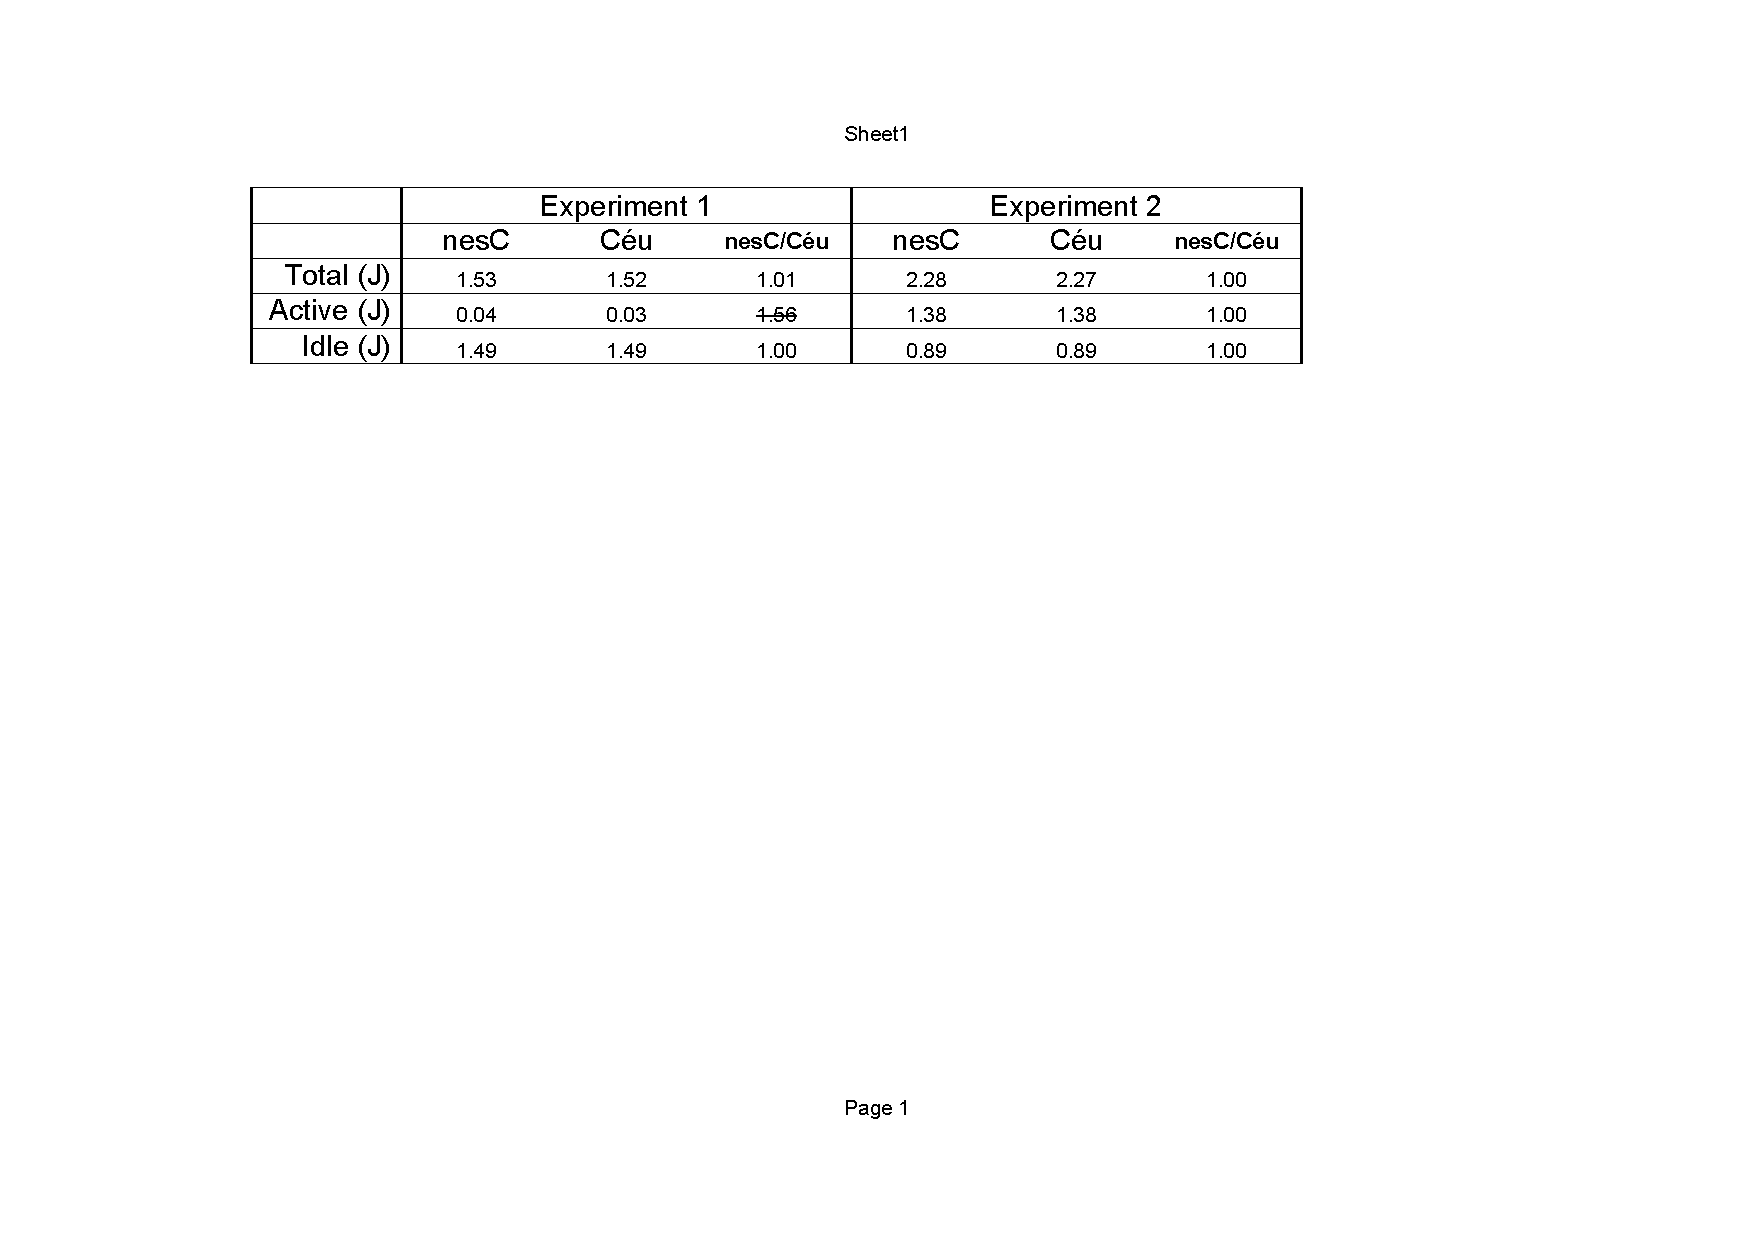
\includegraphics[width=\textwidth,clip=true,trim=120px 415px 210px 90px]{batt}
\caption{ Battery consumption for \emph{nesC} and \CEU in the two experiments.
\newline
{\small %\textmd{
The consumption line "Active" for the Experiment 1 is negligible, hence, the 
ratio between \emph{nesC} and \CEU should not be considered.
}%}
\label{fig.batt}
}
\end{figure*}

We did not expect a noticeable difference in battery usage between \CEU and 
\emph{nesC}, because, even considering the support for multiple lines of 
execution in \CEU, the compiler generates simple event-driven code in $C$, not 
requiring threads or complex runtime apparatus.
%
In fact, the results are virtually the same for both I/O and CPU-bound 
experiments.

\section{Discussion}

\CEU targets control-intensive applications and provides abstractions that can 
express program flow specifications concisely.
%
Our evaluation shows a considerable decrease in code size that comes from 
logical compositions of trails through the \code{par/or} and \code{par/and} 
constructs.
%
They handle startup and termination for trails seamlessly without extra 
programming efforts.
%
We believe that the small overhead in memory qualifies \CEU as a realistic 
option for constrained devices.
%
% TODO:
%Support for local variables did not lead to reduction in RAM, they and
%are and increase .
%
% TODO
%with overheads below 5\% and 10\%
%Some overhead in memory exists, but RAM is minimal and can be avoided XXX an 
%trackable
%inherent per-trail overhead.
%
%The overhead in ROM is below 10\% but has not .
%
%The main aspect of \CEU is to ensure that the high degree of concurrency in 
%WSNs does not pose safety threats to applications.
%
Furthermore, our broad safety analysis, encompassing all proposed concurrency 
mechanisms, ensures that the high degree of concurrency in WSNs does not pose 
safety threats to applications.
%
%Even with the restrictions that were needed to enable this analysis, \CEU was 
%shown to be expressive enough to imply in a decrease in code complexity for a 
%range of typical WSN applications.
%
%By restricting the expressiveness of the language, we could enable a broad 
%safety analysis in programs at compile time.
%The analysis encompasses all proposed concurrency mechanisms, such as parallel 
%compositions, first-class timers, and communication via events.
%
As a summary, the following safety properties hold for all programs that 
successfully compile in \CEU:

\begin{itemize}
\item Time-bounded reactions to the environment
        (Sections~\ref{sec.ceu.det}~and~\ref{sec.ceu.ints}).
\item Reliable weak and strong abortion among activities
        (Sections~\ref{sec.ceu.det}~and~\ref{sec.ceu.shared}).
\item No concurrency in accesses to shared variables
(Section~\ref{sec.ceu.shared}).
\item No concurrency in system calls sharing a resource
        (Section~\ref{sec.ceu.c}).
\item Finalization for blocks going out of scope
        (Section~\ref{sec.ceu.fins}).
\item Auto-adjustment for timers in sequence
        (Section~\ref{sec.ceu.wclocks}).
\item Synchronization for timers in parallel
        (Section~\ref{sec.ceu.wclocks}).
\end{itemize}

These properties are desirable in any application and are guaranteed as 
preconditions in \CEU by design.
Ensuring or even extracting these properties from less restricted languages 
requires significant manual analysis.

Even though the achieved expressiveness and overhead of \CEU meet the 
requirements of WSNs, its design imposes two inherent limitations:
the lack of dynamic loading which would forbid the static analysis,
and the lack of hard real-time guarantees.
%
Regarding the first limitation, dynamic features are already discouraged due to 
resource constraints.
For instance, even object-oriented languages targeting WSNs forbid dynamic 
allocation~\cite{wsn.flowtalk,wsn.virgil}.

To deal with the second limitation, which can be critical in the presence of 
lengthy computations, we can consider the following approaches:
(1) manually placing \code{pause} statements in unbounded loops;
(2) integrating \CEU with a preemptive system.
%
The first option requires the lengthy operations to be rewritten in \CEU using
\code{pause} statements so that other trails can be interleaved with them.
This option is the one recommended in many related work that provide a similar 
cooperative primitive (e.g. \code{pause}~\cite{esterel.primer}, 
\code{PT\_YIELD}~\cite{wsn.protothreads}, \code{yield}~\cite{wsn.sol}, 
\code{post}~\cite{wsn.nesc}).
%
Considering the second option, \CEU and preemptive threads are not mutually 
exclusive.
% and the second option is appealing to be explored in a future work.
For instance, TOSThreads~\cite{wsn.tosthreads} proposes a message-based 
integration with \emph{nesC} that is safe and matches the semantics of \CEU 
external events.

%%%%%%%%%%%%%%%%%%%%%%%%%%%%%%%%%%%%%%%%%%%%%%%%%%%%%%%%%%%%%%%%%%%%%%%%%%%%%%%

\begin{comment}

In order to evaluate the current implementation of \CEU{}, we performed initial
experiments in the domain of Wireless Sensor Networks%
\footnote{The complete source code for the evaluation can be found at \\
\url{http://www.ceu-lang.org/TR/\#exp1}.}.
Our goal is to compare \CEU{} with other languages implementations regarding 
two important aspects for WSNs: \emph{memory usage} and \emph{responsiveness}%
\footnote{Responsiveness is the ability of a system to promptly acknowledge 
high-priority requests (e.g. radio messages).}.

\textbf{Memory usage}

\newcommand{\dif}{{\small \CEU{}--\nesc{}}}
\newcommand{\s}[1]{{\small \textbf{#1}}}

%TODO: basestation_buffer

\begin{table}[t]\small
\begin{center}
\begin{tabular}{ | l | r | r | r | r | }
\hline
\multicolumn{2}{|c|}{}
           &          ROM &         RAM \\
\hline\hline
\multirow{3}{*}{Blink}
    & \nesc &  2048 bytes &    51 bytes \\
    & \CEU  &  5882 bytes &   168 bytes \\
    & \dif  &    \s{3834} &     \s{117} \\
\hline\hline
\multirow{3}{*}{Sense}
    & \nesc &  4366 bytes &    84 bytes \\
    & \CEU  &  8086 bytes &   195 bytes \\
    & \dif  &  \s{3720}   &     \s{111} \\
\hline\hline
\multirow{3}{*}{Client}
    & \nesc & 11838 bytes &   329 bytes \\
    & \CEU  & 15328 bytes &   482 bytes \\
    & \dif  &    \s{3490} &     \s{153} \\
\hline\hline
\multirow{3}{*}{Server}
    & \nesc & 14648 bytes &   373 bytes \\
    & \CEU  & 15686 bytes &   443 bytes \\
    & \dif  &    \s{1038} &      \s{70} \\
\hline
\end{tabular}
\end{center}
\caption{\CEU{} vs TinyOS: memory usage}
\label{tab:eval}
\end{table}

In the first experiment, we ported preexisting \nesc applications to \CEU.
We chose \nesc{} given its popularity in the context of WSNs, and because it is 
event based, consuming less memory than multithreaded languages.
By using preexisting applications in our experiment, we intend not to choose 
specific scenarios that favor one language or the other.

Table~\ref{tab:eval} shows the amount of ROM and RAM for the same applications 
written in \nesc{} and \CEU{}.
The third line for each application shows the difference for a given measure, 
for example: the Client application written in \CEU{} uses $3490$ more bytes 
than its \nesc{} counterpart.

Our experiment suggests that as application complexity grows, the memory 
footprint of \CEU{} becomes diluted, and the difference in consumption 
decreases, showing that \CEU{} is a viable alternative.

%TODO
%Note that \CEU{} already runs on top of \nesc{}, so in theory, the difference 
%should never , which already queues, extra mem we have no control

\textbf{Responsiveness}

\begin{table}[t]\small
\begin{center}
\begin{tabular}{ | l | l | c | c | }
\hline
\multicolumn{2}{|c|}{}
               & no comp. &    5 loops \\
\hline\hline
\multirow{2}{*}{1 sender}
    & MantisOS &  $23.2s$ &    $23.3s$ \\
    & \CEU     &  $23.3s$ &    $23.3s$ \\
\hline\hline
\multirow{2}{*}{2 senders}
    & MantisOS &  $19.8s$ &   $19.9s$ \\
    & \CEU     &  $12.3s$ &   $12.4s$ \\
\hline
\end{tabular}
\\
{\scriptsize\emph{(the measures are the average of three consecutive 
executions)}}
\caption{\CEU{} vs MantisOS: responsiveness}
\label{tab:resp}
\end{center}
\end{table}

In the second experiment, we measure how fast motes can answer radio requests 
when subjected to long computations.
We chose to compare \CEU{} with MantisOS~\cite{wsn.mantisos}, given that 
multithreaded systems perform better in this aspect \cite{wsn.comparison}.
Table~\ref{tab:resp} summarizes the results of this experiment, which is 
described next.

Initially, we created two simple applications that send and receive radio 
messages---with no processing in parallel---to measure how fast they exchange 
$3000$ messages without losses.
We varied the sending speed, and the fastest the receiving side could sustain 
without losses was around $7$ms for each message (coincidentally, in both 
implementations), resulting in $23$s for the entire process 
(\emph{``1~sender/no~comp.''} in Table~\ref{tab:resp}).

In order to evaluate the responsiveness of the receiving side, we changed it to 
also execute in parallel five infinite loops that run forever (to represent 
long computations).
In both \CEU{} and MantisOS implementations, the $3000$ messages were still 
received without losses, while the increase in the total receiving time was 
negligible
(\emph{``1~sender/5~loops''} in Table~\ref{tab:resp}).

In MantisOS, we had to change the priority of the receiving thread to be higher 
than the others.
In \CEU{} the receiving part (which is synchronous) already runs with higher 
priority than long computations (which run inside \emph{asyncs}).

In another test, we kept the single receiver and used two senders to measure 
how fast the receiving side receives $3000$ messages (now ignoring the losses) 
while running long computations in parallel.

Although \CEU{} performs better than MantisOS (probably due to TinyOS higher 
performance), our objective is to measure the \emph{increase} in the total time 
due to the long computations running in parallel.
Again the increase in time is negligible in both implementations.
(\emph{``2~senders''} in Table~\ref{tab:resp}).

From the second experiment, we conclude that \CEU{} is comparable to a 
multithreaded implementation in terms of responsiveness, both having nearly 
optimal behavior for the tests we performed.
Although not in the scope of this work, we asserted that, for all tests, both 
implementations performed a fair scheduling among long computations.

\end{comment}


\chapter{The semantics of C\'eu}
    \label{sec.formal}
    \begin{comment}

\documentclass[11pt,a4paper]{article}
\usepackage[body={6.0in, 8.2in},left=1.25in,right=1.25in]{geometry}

\usepackage{fancyvrb}
\usepackage{verbatim}

\usepackage[pdftex]{graphicx}
\usepackage{subfigure}

\usepackage{listings}
\lstset{frame=tb}
\lstset{basicstyle=\scriptsize}
\lstset{tabsize=4}

\usepackage{amssymb}
\usepackage{amsmath}
\usepackage{amsfonts}
\usepackage{amsthm}

\newcommand{\1}{\;}
\newcommand{\2}{\;\;}
\newcommand{\3}{\;\;\;}
\newcommand{\5}{\;\;\;\;\;}
\newcommand{\ten}{\5\5}
\newcommand{\twenty}{\ten\ten}

\newcommand{\CEU}{\textsc{C\'{e}u}}
\newcommand{\code}[1] {{\small{\texttt{#1}}}}

\newcommand{\ST}{\xrightarrow[i]{}}
\newcommand{\BT}{\xRightarrow[(i,E)]{}}

\begin{document}

\section{Formalization of \CEU}

\end{comment}

\subsection{Abstract syntax}
\label{sec.sem.syntax}

Figure~\ref{lst:ceu:syn} shows the syntax for a subset of \CEU that is 
sufficient to describe all semantic peculiarities of the language.

\begin{figure}[t]
%\rule{8.5cm}{0.37pt}
{\small
\begin{verbatim}
  // primary primitives         // description
  nop(v)                        (constant value)
  mem                           (any memory access)
  await(e)                      (await event `e')
  emit(e)                       (emit event `e')
  break                         (loop escape)

  // compound statements
  if mem then p else q          (conditional)
  p ; q                         (sequence)
  loop p                        (repetition)
  p and q                       (par/and)
  p or q                        (par/or)

  // derived by semantic rules
  awaiting(e)                   (previously awaiting `e')
  stacked(i)                    (stack depth mark)
  emitting(i,e)                 (emitting `e')
  p @ loop p                    (unwinded loop)
\end{verbatim}
}%
\caption{ Simplified syntax of \CEU.
\label{lst:ceu:syn}
}
\end{figure}

A $nop$ represents a terminated computation associated with a constant value.
The $mem$ primitive represents any memory accesses, assignments, and $C$ 
function calls.
As the challenging parts of \CEU reside on its control structures, we are not 
concerned here with a precise semantics for side effects, but only with their 
occurrences in programs.
We refer back to side effects when discussing determinism in 
Section~\ref{sec.safety.det}.

The $await$ and $emit$ primitives are responsible for the reactive nature of 
\CEU.
An $await$ can refer either to an external or internal event, while an $emit$ 
can only refer to an internal event.

The semantic rules to be presented generate three statements that the 
programmer cannot write:
the primitives $awaiting$, $stacked$, and $emitting$ avoid the immediate 
matching of emits and awaits and are used as an artifice to provide the desired 
stacked behavior for internal events.
A $loop$ is expanded with the special \code{`@'} separator (instead of 
\code{`;'}) to properly bind $break$ statements inside $p$ to the enclosing 
loop.
\subsection{Operational semantics}
\label{sec.sem}

In the remaining of this section, we present an operational semantics to 
formally describe a \emph{reaction chain} in \CEU, i.e., how a program behaves 
in reaction to a single external event.%
\footnote{We could extend the semantics to describe the full execution of a 
program by holding new incoming external events in a queue and processing them 
in consecutive reaction chains that never overlap.}

The semantics is split in two sets of rules: \emph{big-step} and 
\emph{small-step} rules.
First, we apply a single big step to awake all trails awaiting the broadcast 
external event.
Then, we continuously apply small steps until all trails await and/or emit.
The next big step awakes all previously awaiting trails matching the emits at 
once.
The two set of rules are interleaved to achieve a complete reaction chain, 
terminating when the program either terminates or awaits in all trails.

In order to provide the desired stacked execution for internal events, the 
semantic rules are associated with an index $i$ that represents the current 
runtime stack depth level.
An emit creates a deeper level $i+1$ and is deferred to be matched in the next 
big step.
The emit continuation (i.e., the statement that follows the emit) remains at 
stack level $i$, as it can only execute after the program completely reacts to 
the event.
Awakened trails may emit new events that will increase the stack depth ($i+2$ 
and so on);
hence, only after the stack unrolls to depth $i$ that the original emitting 
trail continues.

A complete reaction chain to an external event is formalized as follows:
%
$$
%p \xrightarrow[big]{(i,E) = (0,\{ext\})}  \3
(\3
p                                        \1
    \xRightarrow[~(i,E)=pop(p)~]{}     \1
p'
    \xrightarrow[~~i~~]{~~*~~}           \1
p''
\3)*
$$

A big step is represented with the double arrow, where the tuple $(i,E)$ is the 
set $E$ of emitting events to be matched at deepest depth $i$.

For the initial big step, function $pop$ returns the single external event 
emitted at starting depth $1$.
For further big steps, $pop$ is defined in Figure~\ref{fig:pop} and returns the 
deepest stack level and all emitted internal events (if any) from the previous 
small-step sequence.
%
%\footnote{$pop$ needs only to be defined for blocked primitives ($awaiting$ 
%and $stacked$), as small-step sequences that precede big steps always reach 
%these primitives.}
% TODO: colocar na definicao

\begin{figure}[t]
{\small
\begin{align*}
  pop(awaiting(e))   &= (-1, \{\})              \\
  pop(stacked(i))    &= ( i, \{\})              \\
  pop(emitting(i,e)) &= ( i, \{e\})             \\
  pop(p~;~q)         &= pop(p)                  \\
  pop(p~@~loop~q)    &= pop(p)                  \\
  pop(p~and/or~q)    &= (max(j,k), F\cup{}G)    \\
                     & \ten where~(j,F)=pop(p)  \\
                     & \ten\2\2 and~(k,G)=pop(q)
\end{align*}
\emph{(*) Other primitives (nop,mem,await,emit,break,if,loop) do not apply.}
}%
\caption{ The recursive definition for $pop$.
\label{fig:pop}
}
\end{figure}

A small-step sequence is represented with the single arrow and is associated 
with the same depth $i$ from the previous big step, which identifies the 
current (deepest) stack depth.

The sets of rules are interleaved until one of the two possible terminating 
conditions for a reaction chain apply:

\begin{itemize}
\item The program is awaiting in all trails, i.e., function $pop$ returns 
$(-1,\{\})$.
\item The program terminates, i.e., the small-step rules transform the whole 
program into a $nop$.
\end{itemize}
%
In Section~\ref{sec.safety.bounded} we show that, by imposing syntactic 
restrictions to programs, reaction chains always reach one of these conditions 
in a finite number of steps, meaning that reactions to the environment always 
execute in bounded time.

To be compliant with the reactive nature of \CEU, we assume that all programs 
start awaiting the main event ``$\$$'', which is emitted once by the 
environment on startup, i.e., $(i,E)=(1,\{\$\})$ for the very first big step.

\subsubsection{Small-step rules}
\label{sec.sem.small}

As briefly introduced, small-step rules continuously apply transformations to 
unblocked trails.
A program becomes blocked when all parallel branches are hanged in $awaiting$, 
$stacked$, and/or $emitting$ primitives, as defined in 
Figure~\ref{fig:isBlocked}.

% TODO: [|

\begin{figure}[t]
{\small
\begin{align*}
  isBlocked(awaiting(e))   &= true                             \\
  isBlocked(stacked(i))    &= true                             \\
  isBlocked(emitting(i,e)) &= true                             \\
  isBlocked(p~;~q)         &= isBlocked(p)                     \\
  isBlocked(p~@~loop~q)    &= isBlocked(p)                     \\
  isBlocked(p~and~q)       &= isBlocked(p) \wedge isBlocked(q) \\
  isBlocked(p~or~q)        &= isBlocked(p) \wedge isBlocked(q) \\
  isBlocked(*)             &= false \2  (nop,mem,await,        \\
                           &    \5\5\5\2 emit,break,if,loop)   %\\
\end{align*}
}%
\caption{ The recursive predicate $isBlocked$.
\label{fig:isBlocked}
}
\end{figure}

All small-step rules are associated with the current (deepest) stack depth 
level $i$ acquired from the previous big step.

We start with the small-step rules for the primary primitives:
%
\begin{eqnarray*}
& mem \ST nop(v),~~(v~is~nondet)
    & \textbf{(mem)}        \\
%%%
& await(e) \ST stacked(0)~;~awaiting(e)
    & \textbf{(await)}      \\
%%%
& emit(e) \ST emitting(i+1,e)~;~stacked(i)
    & \textbf{(emit)}       %\\
\end{eqnarray*}

A $mem$ operation terminates with a nondeterministic value (e.g., the value of 
a variable or a $C$ function call).

An $await$ is stacked with the lowest possible depth, being transformed in an 
$awaiting$ only in the end of the reaction chain.
This way, a trail that reaches an $await$ can only react to an $emit$ that 
occurs in further reaction chains.

An $emit$ is deferred to a deeper depth to be applied in the next big step.
The rule actually transforms an $emit$ in two primitives in sequence:
the $emitting(i+1,e)$ defers the immediate matching, while $stacked(i)$ holds 
the trail in the current depth, resuming only after the complete reaction to 
the event.

Given that small-step rules execute at the current deepest level and that rule 
\textbf{emit} is the only one that increases the stack depth, the next big step 
will necessarily take all deferred emits.
This explains why the definition for $pop$ in Figure~\ref{fig:pop} blindly 
takes the union of all emitted events without considering their depths.

All other primitives ($nop$, $break$, $awaiting$, $stacked$, and $emitting$) 
represent terminated or blocked trails and, therefore, have no associated 
small-step rules.

The rules for conditionals and sequences are straightforward:
%
\begin{eqnarray*}
& \frac
    { m \ST m' }
% -----------------------------------------------------------
    { (if~m~then~p~else~q) \ST (if~m'~then~p~else~q) }
    & \textbf{(if-adv)}       \\
%%%
& (if~nop(v)~then~p~else~q) \ST p \1,\3 (v \neq 0)
    & \textbf{(if-true)}       \\
%%%
& (if~nop(0)~then~p~else~q) \ST q
    & \textbf{(if-false)}       %\\
%%%
%& (if~mem~then~p) \ST (if~mem~then~p~else~nop)
    %& \textbf{(if-else)}
\end{eqnarray*}
%%%
\begin{eqnarray*}
& \frac
    { p \ST p' }
%   -----------------------------------------------------------
    { (p~;~q) \ST (p'~;~q) }
    & \textbf{(seq-adv)}      \\
%%%
& (nop~;~q) \ST q
    & \textbf{(seq-cst)}      \\
%%%
& (break~;~q) \ST break
    & \textbf{(seq-brk)}     %\\
\end{eqnarray*}
%
%A conditional proceeds to either $p$ or $q$, depending on the evaluation of 
%$mem$ (rules \textbf{if-true} and \textbf{if-false}).
%Note that an empty $else$ branch is substituted by a $nop$ (rule 
%\textbf{if-else}).
%
%Rule \textbf{seq-1} advances composition $p$ until it becomes either a $nop$ 
%(proceeding to $q$ in rule \textbf{seq-2}), or a $break$ (ignoring $q$ in rule 
%\textbf{seq-3}).

Given that the semantics focus on control, note that rules \textbf{if-true} and 
\textbf{if-false} are the only to query $nop$ values.
For all other rules, we omit these values (e.g., \textbf{seq-cst}).

The rules for loops are analogous to sequences, but use \code{`@'} as 
separators to properly bind breaks to their enclosing loops:
%
\begin{eqnarray*}
& { (loop~p) \ST (p~@~loop~p) }
    & \textbf{(loop-expd)}       \\
%%%
& \frac
    { p \ST p' }
% -----------------------------------------------------------
    { (p~@~loop~q) \ST (p'~@~loop~q) }
    & \textbf{(loop-adv)}    \\
%%%
& (nop~@~loop~p) \ST loop~p
    & \textbf{(loop-cst)}    \\
%%%
& (break~@~loop~p) \ST nop
    & \textbf{(loop-brk)}
\end{eqnarray*}

When a program first encounters a $loop$, it first expands its body in sequence 
with itself (rule \textbf{loop-expd}).
Rules \textbf{loop-adv} and \textbf{loop-cst} are similar to rules 
\textbf{seq-adv} and \textbf{seq-cst}, advancing the loop until it reaches a 
$nop$.
However, what follows the loop is the loop itself (rule \textbf{loop-cst}).
Rule \textbf{loop-brk} escapes the enclosing loop, transforming everything into 
a $nop$.
Note that if we used \code{`;'} as a separator in loops, rules 
\textbf{loop-brk} and \textbf{seq-brk} would conflict.

The small-step rules for parallel compositions advance trails independently and 
require that both sides either block or terminate.
% to advance to the next big step.
For an $and$, if one of the sides terminate, the composition is simply
substituted by the other side.
For an $or$, if one of the sides terminate, the other side must advance until 
it blocks.
Then, the whole composition terminates and the blocked side is \emph{killed}, 
i.e., all its $awaiting$, $stacked$, and $emitting$ primitives are eliminated 
with the rule transformation.

A similar situation occurs when an $and$ or $or$ reach a $break$ in either of 
the sides.
In this case, the enclosing $loop$ must terminate and both sides are killed, 
transforming the whole composition into a $break$.
As the rules make explicit, a trail can only be killed after it terminates or 
blocks.

Follow the rules for a parallel $and$:
%
\begin{eqnarray*}
& \frac
    { p \ST p' }
%   -----------------------------------------------------------
    { (p~and~q) \ST (p'~and~q) }
    & \textbf{(and-adv1)}      \\
%%%
& \frac
    { q \ST q' }
%   -----------------------------------------------------------
    { (p~and~q) \ST (p~and~q') }
    & \textbf{(and-adv2)}      \\
%\end{eqnarray*}
%%%
%\begin{eqnarray*}
& (nop~and~q) \ST q
    & \textbf{(and-cst1)}   \\
%%%
& (p~and~nop) \ST p
    & \textbf{(and-cst2)}   \\
%%%
& \frac
    { q=break \1\vee\1 isBlocked(q) }
%   -----------------------------------------------------------
    { (break~and~q) \ST break }
    & \textbf{(and-brk1)}   \\
%%%
& \frac
    { p=break \1\vee\1 isBlocked(p) }
%   -----------------------------------------------------------
    { (p~and~break) \ST break }
    & \textbf{(and-brk2)}   %\\
\end{eqnarray*}

Rules \textbf{and-cst1} and \textbf{and-cst2} handle the termination of one of 
the sides, substituting the whole composition by the other side.
Rules \textbf{and-brk1} and \textbf{and-brk2} handle the special case for 
reaching a $break$, in which the other blocked side is killed by transforming 
the whole composition becomes into a $break$ to terminate the enclosing loop.
For instance, the program \code{loop(break~and~emit(a))} never emits $a$, 
because the $emit$ blocks (rule \textbf{emit}) and is then killed (rule 
\textbf{and-brk1}).

The rules for a parallel $or$ are slightly different:
%
\begin{eqnarray*}
& \frac
    { p \ST p' }
%   -----------------------------------------------------------
    { (p~or~q) \ST (p'~or~q) }
    & \textbf{(or-adv1)}   \\
%%%
& \frac
    { q \ST q' }
%   -----------------------------------------------------------
    { (p~or~q) \ST (p~or~q') }
    & \textbf{(or-adv2)}   \\
%%%
& \frac
    { q=nop \1\vee\1 isBlocked(q) }
%   -----------------------------------------------------------
    { (nop~or~q) \ST nop }
    & \textbf{(or-cst1)}   \\
%%%
& \frac
    { p=nop \1\vee\1 isBlocked(p) }
%   -----------------------------------------------------------
    { (p~or~nop) \ST nop }
    & \textbf{(or-cst2)}   \\
%%%
& \frac
    { q=nop \1\vee\1 q=break \1\vee\1 isBlocked(q) }
%   -----------------------------------------------------------
    { (break~or~q) \ST break }
    & \textbf{(or-brk1)}   \\
%%%
& \frac
    { p=nop \1\vee\1 p=break \1\vee\1 isBlocked(p) }
%   -----------------------------------------------------------
    { (p~or~break) \ST break }
    & \textbf{(or-brk2)}   %\\
\end{eqnarray*}

Rules \textbf{or-cst1} and \textbf{or-cst2} terminate the $or$ when at least 
one of the sides is a $nop$.
For instance, the program \code{loop(nop~and~emit(a))} never emits $a$, because 
the $emit$ blocks (rule \textbf{emit}) and is then killed (rule 
\textbf{or-cst1}).
%Note that these rules enforce both sides to advance until they either 
%terminate or block.
%, what necessarily happens because all unblocked primitives have associated 
%small-step rules.
Rules \textbf{or-brk1} and \textbf{or-brk2} are similar to their $and$ 
counterparts, with the additional remark that a $break$ has preference over a 
$nop$, i.e., when they appear on each side, the whole composition becomes a 
$break$ instead of a $nop$.

%(TODO: orthogonal preemption)

Note that rule \textbf{mem} and the pairs \textbf{and-adv1}/\textbf{and-adv2} 
and \textbf{or-adv1}/\textbf{or-adv2} bring nondeterminism to the semantics of 
\CEU.
%Also, rule \textbf{loop-exp} may expand the program indefinitely, leading to 
%unbounded execution for \CEU programs.
However, in Section~\ref{sec.safety.det} we discuss how to detect programs with 
deterministic behavior (even with nondeterminism in $mem$ operations and 
scheduling), refusing all other programs at compile time.

\subsubsection{Big-step rules}
\label{sec.sem.big}

The big-step semantics matches $emitting$ and $awaiting$ trails, providing 
broadcast communication in the language.
It is important to use a big-step operational semantics in order to apply 
transformations in parallel, all at once.
Emits with no matching awaits are simply discarded, characterizing the 
unbuffered communication typically adopted in synchronous languages.

Big-step rules are associated with a tuple $(i,E)$ that represents the set of 
occurring events $E$ triggered at stack depth $i$.

\begin{comment}
At the beginning of each reaction chain, only a single external event can be 
active, as required by \CEU's synchronous execution model.
Hence, initially $(i,E) = (0,\{ext\})$, where $ext$ is the external event 
triggered at starting depth $0$.

For further big steps following small steps, the tuple $(i,E)$ is acquired from 
the recursive function $pop$, which takes the deepest stack depth and groups 
all stacked emits (if any) together:

As explained for small-step rule \textbf{emit}, all stacked emits necessarily 
occur at deepest depth.
Note also that $pop$ does not need to be defined for unblocked primitives, as a 
small-step sequence that precedes a big step only terminates when the program 
becomes blocked.

We now present the big-step semantic rules.
\end{comment}

We start with the rules to check if deferred emits match previously awaiting 
trails:
%
\begin{eqnarray*}
& awaiting(e) \BT nop \1,\3 (e \in E)
    & \textbf{(Await-awk)}    \\
%%%
& awaiting(e) \BT awaiting(e) \1,\3 (e \notin E)
    & \textbf{(Await-rep)}    \\
\end{eqnarray*}

The $stacked$ and $emitting$ primitives are ``popped'' if they are at the 
deepest level $i$ returned by function $pop$:

\begin{eqnarray*}
& stacked~(i) \BT nop \5
    & \textbf{(Stack)}  \\
%
& emitting~(i,e) \BT nop \5
    & \textbf{(Emitting)}  %\\
\end{eqnarray*}

\begin{comment}
A deferred emit cannot unblock immediately because the just matched trails 
(rule \textbf{Await-awk}) must all react before the emit continuation proceeds.
Hence, rule \textbf{Stack} specifies that the emit continuation remains blocked 
at the same (low) depth.
This way, awaken trails will execute in the next small-step sequence and new 
emits will be deferred at deeper depths (note the \code{i+1} in small-step rule 
\textbf{emit}).
Eventually, no new emits will take place, and function $pop$ will pop the 
continuations with the highest depth, which will proceed through rule 
\textbf{Cont}, providing the desired stacked execution for internal events.
\end{comment}

To conclude the big-step semantics, the rules for compound statements advance 
their subparts all at once:
%
\begin{eqnarray*}
& \frac
    { p \BT p' }
%   -----------------------------------------------------------
    { (p~;~q) \BT (p'~;~q) }
    & \textbf{(Seq)}    \\
%%%
& \frac
    { p \BT p' }
%   -----------------------------------------------------------
    { (p~@~loop~q) \BT (p'~@~loop~q) }
    & \textbf{(Loop)}   \\
%%%
& \frac
    { p \BT p' \5 q \BT q' }
%   -----------------------------------------------------------
    { (p~and~q) \BT (p'~and~q') }
    & \textbf{(And)}    \\
%%%
& \frac
    { p \BT p' \5 q \BT q' }
%   -----------------------------------------------------------
    { (p~or~q) \BT (p'~or~q') }
    & \textbf{(Or)}     %\\
\end{eqnarray*}

Note that there are no rules for $mem$, $break$, $emit$, $nop$, and $if$ 
because none of these represent blocked primitives, and hence, never appear in 
a big step.

\begin{comment}

\textbf{(TODO) An example:}

{\small
\begin{verbatim}
    mem(1); emit a; mem(2); emit b; mem(3)
or (
    loop (mem(4); await a)
or
    await b; mem(5)
)
\end{verbatim}
}

$$
p = program
\ten
ext = external~event
$$

$$
*^1: \1 until \3 isBlocked(p'') \1\vee\1 (p''=nop)
$$
$$
*^2: \1 until \3 pop(p'')=(0,\emptyset)
$$

\subsection{Examples}

$$
\textbf{(seq)} \5
    \frac
    { \textbf{(await 1)} \3 await~A \xrightarrow{(A,0)} delay~0 }
%   -----------------------------------------------------------
    { (await~A~;~await~A) \xrightarrow{(A,0)} (delay~0~;~await~A) }
$$

$$
\textbf{(seq 1)} \5
    \frac
    {\textbf{(delay)} \5 (delay~0) \xrightarrow{0}
        nop \1\nearrow^{~\emptyset}}
%   -----------------------------------------------------------
    { (delay~0~;~await~A) \xrightarrow{0} (nop~;~await~A)
        \1\nearrow^{~\emptyset} }
$$

$$
\textbf{(seq 2)} \3 (nop~;~await~A) \xrightarrow{i}
                        await~A \1\nearrow^{~\emptyset}
$$

$$
\textbf{(loop 1)} \5
    \frac
    {\textbf{(if)} \5
        (if~...) \xrightarrow{(\_,0)} (if~...)}
%   -----------------------------------------------------------
    { loop~(if~...) \xrightarrow{(\_,0)}
        (if~mem(v)~then~break~else~await~A)~@~loop~(if~...)) }
$$

$$
\textbf{(if 0)} \3
    (if~mem(0)~then~p~else~q) \xrightarrow{i} q \1\nearrow^{~\emptyset}
\ten
\textbf{(if 1)} \3
    (if~mem(v)~then~p~else~q) \xrightarrow{i} p \1\nearrow^{~\emptyset}
        \1,\3 (v \neq 0)
$$

$$
\textbf{(loop 1)} \5
    \frac
    { \textbf{(if 1)} \3
    (if~mem(1)~...) \xrightarrow{0} break \1\nearrow^{~\emptyset} }
%   -----------------------------------------------------------
    { (if~mem(1)~...~@~loop~q) \xrightarrow{0} (break~@~loop~(if~...))
        \1\nearrow^{~\emptyset} }
$$

$$
\textbf{(loop 1)} \5
    \frac
    { \textbf{(if 0)} \3
    (if~mem(0)~...) \xrightarrow{0} await~A \1\nearrow^{~\emptyset} }
%   -----------------------------------------------------------
    { (if~mem(0)~...~@~loop~q) \xrightarrow{0} (await~A~@~loop~(if~...))
        \1\nearrow^{~\emptyset} }
$$

$$
\textbf{(loop 3)} \3
    (break~@~loop~(if~...)) \xrightarrow{0} nop \1\nearrow^{~\emptyset}
$$


$$
\textbf{(loop 2)} \3
    \frac
    { \textbf{(await 1)} \3 await~A \xrightarrow{(A,0)} delay~0 }
%   -----------------------------------------------------------
    { await~A~@~loop~(if~...) \xrightarrow{(e,i)} delay~0~@~loop~(if~...) }
$$

$$
\textbf{(loop 1)} \5
    \frac
    { \textbf{(delay)} \5 (delay~0) \xrightarrow{0} nop
        \1\nearrow^{~\emptyset} }
%   -----------------------------------------------------------
    { delay~0~@~loop~(if~...) \xrightarrow{0} nop~@~loop~(if~...)
        \1\nearrow^{~\emptyset} }
$$

$$
\textbf{(loop 2)} \3
    (nop~@~loop~(if~...) \xrightarrow{0}
        (if~...)~@~loop~(if~...) \1\nearrow^{~\emptyset}
$$

$$
\textbf{(or)} \5
    \frac
    { \textbf{(seq)} \1 ... \xrightarrow{(A,0)} ... \5
        \textbf{(or)} \3
            \frac
            { \textbf{(await~2)} \1 await~b \xrightarrow{(A,0)} await~b \5
                \textbf{(seq)} \1
                    \frac
                    { \textbf{(await~1)} \1 await~A \xrightarrow{(A,0)} delay~0 
}
                %   -----------------------------------------------------------
                    { (await~A~;~emit~a) \xrightarrow{(A,0)} (delay~0~;~emit~a) 
            }
            }
        %   -----------------------------------------------------------
            { (await~b~or~(await~A;emit~a)) \xrightarrow{(A,0)}
                (await~b~or~(delay~0;emit~a)) }
    }
%   -----------------------------------------------------------
    { (...~or~(await~b~or~(await~A;emit~a))) \xrightarrow{(A,0)}
        (...~or~(await~b~or~(delay~0;emit~a))) }
$$

$$
\textbf{(or)} \5
    \frac
    { p \xrightarrow{(e,i)} p' \5 q \xrightarrow{(e,i)} q' }
%   -----------------------------------------------------------
    { (p~or~q) \xrightarrow{(e,i)} (p'~or~q') }
$$

$$
\textbf{(or 2)} \3
    \frac
    { isReady(q,i) \5 q \xrightarrow{i} q' \1\nearrow^{~(e,i)} }
%   -----------------------------------------------------------
    { (...~or~(await~b~or~(delay~0~;~emit~a))) \xrightarrow{0}
        (...~or~nop~;~emit~a) \1\nearrow^{~(e,i)} }
$$

$$
    \frac
    {
        \frac
        {
            \textbf{(seq 1)} \1 \frac {
                \textbf{(delay)} \1 (delay~0) \xrightarrow{0} nop
            }{
                (delay~0;~emit~a) \xrightarrow{0} nop~;~emit~a
            }
        \3
            \textbf{(seq 2)} \1 (nop~;~emit~a) \xrightarrow{0} emit~a
        }
%       -----------------------------------------------------------
        { (delay~0~;~emit~a) \xrightarrow{0} emit~a }
    \3
        \textbf{(emit)} \1 emit~a \xrightarrow{0} delay~1 \1\nearrow^{~(a,2)}
    }
%   -----------------------------------------------------------
    { (delay~0~;~emit~a) \xrightarrow{0} delay~1 \1\nearrow^{~(a,2)} }
$$

(seq 3)
loop do
    par/or do
        se1 ;
        break;
    with
        se2 ;
    end
    se3;
end

- restricao de tight loop é a única na sintaxe
- depois vou fazer a semantica para ND
    - criar um grafo
    - mostrar que é o unico grafo
- com a semantica de ND, também posso "falhar" em caso de tight loop, o que 
  removeria a restricao na sintaxe e daria semantica p/ o tight loop

Prova 1: mostrar que a inclusão de $(f,i+1)$ e $(\_,i+2)$ em E-global na regra 
(emit) não causa problemas, já que as regras em paralelo estão reagindo a "i" e 
a reação a "i+1" só é possível quando todas as outras terminarem (via regra 
step)

Prova 2: provar que eu chego em $S_{\emptyset}$

Prova 3: não é possível fazer infinitas transições
- preciso remover "same" e "nop"

Prova 1 e 2 -> Reaction chain executa em bounded time

\begin{figure}[t]
\begin{eqnarray*}
& mem \xrightarrow{i} nop(v)
    & \textbf{(mem)}        \\
%%%
& emit~e \xrightarrow{i} delay~(e,i+1)
    & \textbf{(emit)}       \\
%%%
& \frac
    { mem \xrightarrow{i} nop(v) \1,\3 (v \neq 0) }
% -----------------------------------------------------------
    { (if~mem~then~p~else~q) \xrightarrow{i} p }
    & \textbf{(if-true)}    \\
%%%
& \frac
    { mem \xrightarrow{i} nop(0) }
% -----------------------------------------------------------
    { (if~mem~then~p~else~q) \xrightarrow{i} q }
    & \textbf{(if-false)}   \\
%%%
& (if~mem~then~p) \xrightarrow{i} (if~mem~then~p~else~nop)
    & \textbf{(if-else)}    \\
%%%
& \frac
    { p \xrightarrow{i} p' }
%   -----------------------------------------------------------
    { (p~;~q) \xrightarrow{i} (p'~;~q) }
    & \textbf{(seq-1)}      \\
%%%
& (nop~;~q) \xrightarrow{i} q
    & \textbf{(seq-2)}      \\
%%%
& (break~;~q) \xrightarrow{i} break
    & \textbf{(seq-3)}      \\
%%%
& { (loop~p) \xrightarrow{i} (p~@~loop~p) }
    & \textbf{(loop-exp)}   \\
%%%
& \frac
    { p \xrightarrow{i} p' }
% -----------------------------------------------------------
    { (p~@~loop~q) \xrightarrow{i} (p'~@~loop~q) }
    & \textbf{(loop-1)}    \\
%%%
& (nop~@~loop~p) \xrightarrow{i} loop~p
    & \textbf{(loop-2)}    \\
%%%
& (break~@~loop~p) \xrightarrow{i} nop
    & \textbf{(loop-3)}     \\
%%%
& \frac
    { p \xrightarrow{i} p' }
%   -----------------------------------------------------------
    { (p~and~q) \xrightarrow{i} (p'~and~q) }
    & \textbf{(and-1)}      \\
%%%
& \frac
    { q \xrightarrow{i} q' }
%   -----------------------------------------------------------
    { (p~and~q) \xrightarrow{i} (p~and~q') }
    & \textbf{(and-2)}      \\
%%%
& (nop~and~q) \xrightarrow{i} q
    & \textbf{(and-3)}      \\
%%%
& (p~and~nop) \xrightarrow{i} p
    & \textbf{(and-4)}      \\
%%%
& \frac
    { q=break \1\vee\1 isBlocked(q) }
%   -----------------------------------------------------------
    { (break~and~q) \xrightarrow{i} break }
    & \textbf{(and-5)}      \\
%%%
& \frac
    { p=break \1\vee\1 isBlocked(p) }
%   -----------------------------------------------------------
    { (p~and~break) \xrightarrow{i} break }
    & \textbf{(and-6)}      \\
%%%
& \frac
    { p \xrightarrow{i} p' }
%   -----------------------------------------------------------
    { (p~or~q) \xrightarrow{i} (p'~or~q) }
    & \textbf{(or-1)}   \\
%%%
& \frac
    { q \xrightarrow{i} q' }
%   -----------------------------------------------------------
    { (p~or~q) \xrightarrow{i} (p~or~q') }
    & \textbf{(or-2)}   \\
%%%
& \frac
    { q=nop \1\vee\1 isBlocked(q) }
%   -----------------------------------------------------------
    { (nop~or~q) \xrightarrow{i} nop }
    & \textbf{(or-3)}   \\
%%%
& \frac
    { p=nop \1\vee\1 isBlocked(p) }
%   -----------------------------------------------------------
    { (p~or~nop) \xrightarrow{i} nop }
    & \textbf{(or-4)}   \\
%%%
& \frac
    { q=nop \1\vee\1 q=break \1\vee\1 isBlocked(q) }
%   -----------------------------------------------------------
    { (break~or~q) \xrightarrow{i} break }
    & \textbf{(or-5)}   \\
%%%
& \frac
    { p=nop \1\vee\1 p=break \1\vee\1 isBlocked(p) }
%   -----------------------------------------------------------
    { (p~or~break) \xrightarrow{i} break }
    & \textbf{(or-6)}   \\
\end{eqnarray*}%
\caption{ Small-step rules. }
\label{lst:ceu:1}
\end{figure}

\end{document}
\end{comment}


\chapter{The implementation of C\'eu}
    \label{sec.impl}
    %\begin{document}

\begin{comment}
As a static language, much of the complexity in the implementation of \CEU{} 
resides in the compile phase.
Nonetheless, some complexity is left to the runtime phase, which has to manage 
first-class timers, finalization blocks, and all bookkeeping related to trails.
\end{comment}

The compilation process of a program in \CEU is composed of three main phases, 
as illustrated in Figure~\ref{fig.impl}:

\begin{figure}[ht]
\centering
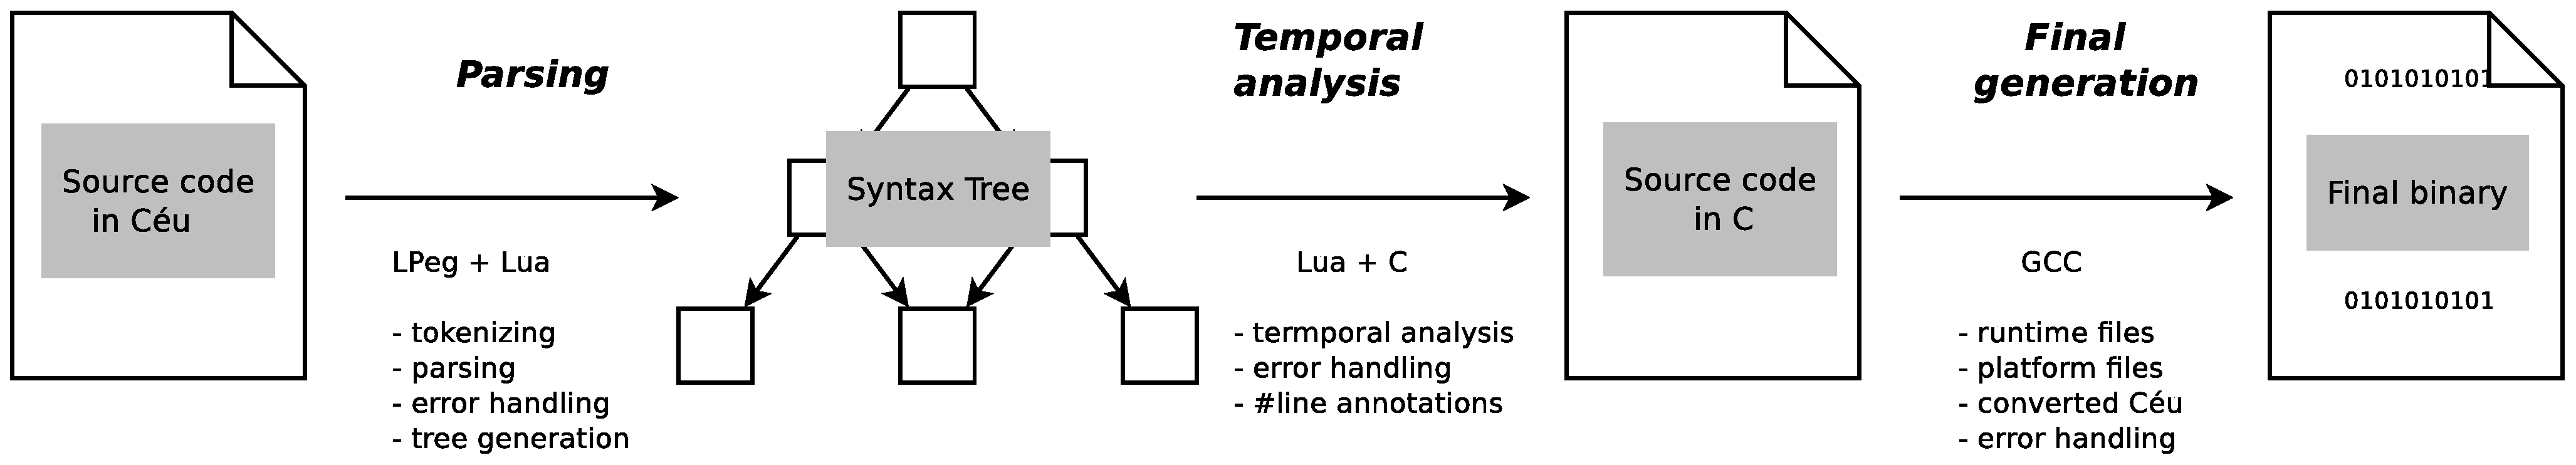
\includegraphics[scale=0.20]{impl}
\caption{ Compilation process: from the source code in \CEU to the final 
binary.
\label{fig.impl}
}
\end{figure}

\begin{comment}
The program below is used as our guiding example for this chapter:

\begin{lstlisting}[numbers=left,xleftmargin=2em]
input int A, B, C;
var int ret;
loop do
   par/or do
      do                            // 1st trail
          var int a = await A;
          ret = ret + a;
      end
      do
          var int b = await B;
          ret = ret + b;
      end
      break;
   with
      par/and do                    // 2nd trail
         finalize with
            ret = ret + 10;
         end
         await C;
      with
         await A;
      end
   end
end
...                                 // code after the loop
\end{lstlisting}
\end{comment}

\begin{description}

\item[Parsing]

The parser of \CEU is written in \emph{LPeg}~\cite{lua.lpeg}, a pattern 
matching library that also recognize grammars, making it possible to write the 
tokenizer and grammar with the same tool.
%
The source code is then converted to an \emph{abstract syntax tree (AST)} to be 
used in further phases.
%
This phase may be aborted due to syntax errors in the \CEU source file.

\item[Temporal analysis]

This phase detects inconsistencies in \CEU programs, such as unbounded loops 
and the forms of non-determinism.
%
It also makes some ``classical'' semantic analysis, such as building a symbol 
table for checking variable declarations.
However, most of type checking is delayed to the last phase to take advantage 
of GCC's error handling.
Therefore, this phase needs to annotate the $C$ output with \code{\#line} 
pragmas that match the original file in \CEU.
%
This phase must output code in $C$, given how tied \CEU is to $C$ by design.

\item[Final generation]

The final phase packs the generated $C$ file with the \CEU runtime and 
platform-dependent functionality, compiling them with \emph{gcc} and generating 
the final binary.
%
The \CEU runtime includes the scheduler, timer management, and the external $C$ 
API.
%
The platform files include libraries for I/O and bindings to invoke the \CEU 
scheduler on external events.

\end{description}

In the sections that follow, we discuss the most sensible parts of the compiler 
considering our design, such as the temporal analysis, runtime scheduler, and 
the external API.

\section{Temporal analysis}

As introduced, the \emph{temporal analysis} phase detects inconsistencies in 
\CEU programs.
Here, we focus on the algorithm that detects non-deterministic access to 
variables, as presented in Section~\ref{sec.ceu.shared}.

For each node representing a statement in the program AST, we keep the set of 
events $I$ (for \emph{incoming}) that can lead to the execution of the node, 
and also the set of events $O$ (for \emph{outgoing}) that can terminate the 
node.

A node inherits the set $I$ from its direct parent and calculates $O$ according 
to its type:
%
\begin{itemize}
%
\item Nodes that represent expressions, assignments, $C$ calls, and 
declarations simply reproduce $O=I$, as they do not await;
%
\item An \code{await e} statement has $O=\{e\}$.
%
\item A \code{break} statement has $O=\{\}$ as it escapes the innermost 
\code{loop} and never terminate, i.e., never proceeds to the statement 
immediately following it (see also \code{loop} below);
%
\item A \emph{sequence node (;)} modifies each of its children to have 
$I_n=O_{n-1}$.
The first child inherits $I$ from the sequence parent, and the set $O$ for the 
sequence node is copied from its last child, i.e., $O=O_n$.
%
\item A \code{loop} node includes its body's $O$ on its own $I$ ($I=I \cup 
O_{body}$), as the loop is also reached from its own body.
The union of all \code{break} statements' $O$ forms the set $O$ for a 
\code{loop}.
%
\item An \code{if} node has $O=O_{true} \cup O_{false}$.
%
\item A parallel composition (\code{par/and} / \code{par/or}) may terminate 
from any of its branches, hence $O = O_1 \cup ... \cup O_n$.
\end{itemize}

With all sets calculated, any two nodes that perform side effects and are in 
parallel branches can have their $I$ sets compared for intersections.
If the intersection is not the empty set, they are marked as suspicious (see 
Section~\ref{sec.ceu.shared}).

Figure~\ref{lst.impl.ast} reproduces the second code of Figure~\ref{lst.det} 
and shows the corresponding $AST$ with the sets $I$ and $O$ for each node.
The event $.$ (dot) represents the ``boot'' reaction.
The assignments to \code{y} in parallel (lines 5,8 in the code) have an empty 
intersection of $I$ (lines 6,9 in the AST), hence, they do not conflict.
Note that although the accesses in lines 5, 11 in the code (lines 6,11 in the 
AST) do have an intersection, they are not in parallel and are also safe.

\begin{figure}[h]
\begin{minipage}[t]{0.45\linewidth}
\begin{lstlisting}
input void A, B;
var int y;
par/or do
  await A;
  y = 1;
with
  await B;
  y = 2;
end
await A;
y = 3;
\end{lstlisting}
\end{minipage}
%
%
\begin{minipage}[t]{0.55\linewidth}
\begin{lstlisting}[numbers=left,xleftmargin=2.5em]
Stmts I={.} O={A}
    Dcl_y I={.} O={.}
    ParOr I={.} O={A,B}
        Stmts I={.} O={A}
            Await_A I={.} O={A}
            Set_y I={A} O={A}
        Stmts I={.} O={B}
            Await_B I={.} O={B}
            Set_y I={B} O={B}
    Await_A I={A,B} O={A}
    Set_y I={A} O={A}
\end{lstlisting}
\end{minipage}
%
\rule{14cm}{0.37pt}
\caption{ A program with a corresponding AST describing the sets $I$ and $O$.
%{\small %\textmd{
The program is safe because accesses to \code{y} in parallel have no 
intersections for $I$.
%}%}
\label{lst.impl.ast}
}
\end{figure}


\begin{comment}
It is also responsible for setting the priorities for trails (see further) and 
determining the sizes of the queues that are used during runtime.

The program AST is first converted into a graph that represents the execution 
flow.
Figure~\ref{fig:nfa} shows the corresponding graph for our example.

\begin{figure}[ht]
\centering
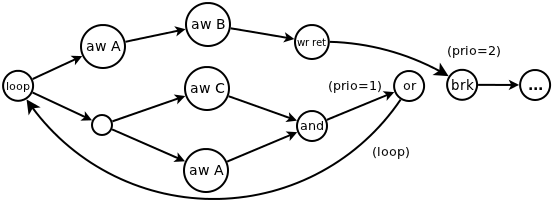
\includegraphics[scale=0.40]{nfa.png}
\caption{ Flow graph for our guiding example
\label{fig:nfa}
}
\end{figure}

By default, all nodes in a flow graph have priority $0$ (highest).
However, as the figure shows, nodes that represent the termination of 
\emph{par/ors} and loops have lower priorities (the outer, the lower).
The priority scheme is needed to avoid glitches during runtime, and is 
equivalent to traversing a dependency graph in topological order, as employed 
in functional reactive programming implementations.~\cite{frtime.embedding}

The flow graph is then converted to a DFA, as exemplified in 
Section~\ref{sec:ceu:det}.

From its starting node, the flow graph is traversed until reaching await 
nodes---every visited node is inserted into a new DFA state.
Then, every set of awaiting nodes for a given external event starts another DFA 
state.
\end{comment}

\section{Memory layout}
\label{sec:impl:memory}

\CEU{} favors a fine-grained use of trails, being common the use of trails that 
await a single event.
For this reason, \CEU{} does not allocate per-trail stacks; instead, all data 
resides in fixed memory slots---this is true for the program variables as well 
as for temporary values and flags needed during runtime.
%For instance, the first trail in the guiding example requires temporary slots 
%to hold the locals \code{a} and \code{b}, while the second trail must keep 
%flags to remember which sides of the \code{par/and} have already terminated.
%
Memory for trails in parallel must coexist, while statements in sequence can 
reuse it.
%In the example, the code following the loop (identified as \code{...}) reuses 
%all memory from the loop.
%
\CEU reserves a single static block of memory to hold all memory slots, whose 
size is the maximum the program uses at a given time.
A given position in the memory may hold different data (with variable sizes) 
during runtime.

\begin{figure}[t]
\begin{minipage}[t]{0.45\linewidth}
\begin{lstlisting}
input int A, B, C;
do
    var int a = await A;
end
do
    var int b = await B;
end
par/and do
    await B;
with
    await C;
end
\end{lstlisting}
\end{minipage}
%
\begin{minipage}[t]{0.55\linewidth}
\begin{lstlisting}
union {             // sequence
    int a_1;        //   do_1
    int b_2;        //   do_2
    struct {        //   par/and
        u8 _and_3: 1;
        u8 _and_4: 1;
    };
} MEM ;
\end{lstlisting}
\end{minipage}
\rule{14cm}{0.37pt}
\caption{
A program with blocks in sequence and in parallel, with corresponding memory 
layout.
{\small %\textmd{
}%}
\label{lst.impl.mem}
}
\end{figure}

Translating this idea to $C$ is straightforward~\cite{wsn.osm,wsn.ocram}: 
memory for blocks in sequence are packed in a \code{struct}, while blocks in 
parallel, in a \code{union}.
%
As an example, Figure~\ref{lst.impl.mem} shows a program with corresponding 
memory layout.
%
Each variable is assigned a unique $id$ (e.g. \code{a\_1}) so that variables 
with the same name can be distinguished.
%
The \code{do-end} blocks in sequence are packed in a \code{union}, given that 
their variables cannot be in scope at the same time, e.g., \code{MEM.a\_1} and 
\code{MEM.b\_2} can safely share the same memory address.
%
The example also illustrates the presence of runtime flags related to the 
parallel composition, which also reside in reusable slots in the static memory.

\section{Trail allocation}
\label{sec:impl:gates}

The compiler extracts the maximum number of trails a program can have at the 
same time and creates a static vector to hold runtime information about them.
Again, trails that cannot be active at the same time can share memory slots in 
the static vector.

At any given moment, a trail can be awaiting in one of the following states: 
\code{INACTIVE}, \code{STACKED}, \code{FIN}, or in any event defined in the 
program:

\begin{lstlisting}
enum {
    INACTIVE = 0,
    STACKED,
    FIN,
    EVT_A,      // input void A;
    EVT_e,      // event int e;
    <...>       // other events
}
\end{lstlisting}

All terminated or not-yet-started trails stay in the \code{INACTIVE} state and 
are ignored by the scheduler.
%
A \code{STACKED} trail holds its associated stack level and is delayed until 
the scheduler runtime level reaches that value again.
%
A \code{FIN} trail represents a hanged finalization block which is only 
scheduled when its corresponding block goes out of scope.
%
A trail waiting for an event stays in the state of the corresponding event, 
also holding the sequence number (\emph{seqno}) in which it started awaiting.
%
A trail is represented by the following \code{struct}:

\begin{lstlisting}
struct trail_t {
    state_t evt;
    label_t lbl;
    union {
        unsigned char seqno;
        stack_t       stk;
    };
};
\end{lstlisting}

The field \code{evt} holds the state of the trail (or the event it is 
awaiting); the field \code{lbl} holds the entry point in the code to execute 
when the trail is scheduled; the third field depends on the \code{evt} field 
and may hold the \code{seqno} for an event, or the stack level \code{stk} for a
\code{STACKED} state.

The size of \code{state\_t} depends on the number of events in the application;
for an application with less than 253 events (plus the 3 states), one byte is 
enough.
%
The size of \code{label\_t} depends primarily on the number of \code{await} 
statements in the application---each \code{await} splits the code in two and 
requires a unique entry point in the code for its continuation.
Additionally, split \& join points for parallel compositions, \code{emit} 
continuations, and finalization blocks also require labels.
%
The \code{seqno} will eventually overflow during execution (every 256 
reactions).
However, given that the scheduler traverses all trails in each reaction, it can 
adjust them to properly handle overflows (actually 2 bits to hold the 
\code{seqno} would be already enough).
%
The stack size depends on the maximum depth of nested emissions and is bounded 
to the maximum number of trails, e.g., a trail emits an event that awakes 
another trail, which emits an event that awakes another trail, and so on---the 
last trail cannot awake any trail, because they will be all hanged in a 
\code{STACKED} state.
%
In WSNs applications, the size of \code{trail\_t} is typically only 3 bytes (1 
byte for each field).

\subsection{Code generation}

\begin{figure}[t]
\begin{minipage}[t]{0.55\linewidth}
\begin{lstlisting}[numbers=left,xleftmargin=2em]
input void A;
event void e;
// TRAIL 0 - lbl Main
par/and do
  // TRAIL 0 - lbl Main
  await e;
  // TRAIL 0 - lbl Awake_e
  // TRAIL 0 - lbl ParAnd_chk
with
  // TRAIL 1 - lbl ParAnd_sub_2
  await A;
  // TRAIL 1 - lbl Awake_A_1
  emit e;
  // TRAIL 1 - lbl Emit_e_cont
  // TRAIL 1 - lbl ParAnd_chk
end
// TRAIL 0 - lbl ParAnd_out
await A;
// TRAIL 0 - lbl Awake_A_2
\end{lstlisting}
\end{minipage}
%
\begin{minipage}[t]{0.45\linewidth}
\begin{lstlisting}
enum {
  Main = 1,     // ln  3
  Awake_e,      // ln  7
  ParAnd_chk,   // ln  8, 15
  ParAnd_sub_2, // ln 10
  Awake_A_1,    // ln 12
  Emit_e_cont,  // ln 14
  ParAnd_out,   // ln 17
  Awake_A_2     // ln 19
};
\end{lstlisting}
\end{minipage}
\rule{14cm}{0.37pt}
\caption{
%{\small %\textmd{
Static allocation of trails and entry-point labels.
%}%}
\label{lst.impl.trails}
}
\end{figure}

The example in Figure~\ref{lst.impl.trails} illustrates how trails and labels 
are statically allocated in a program.
%
The program has a maximum of 2 trails, because the \code{par/and} (line 4) can 
reuse \emph{TRAIL 0}, and the join point (line 16) can reuse both \emph{TRAIL 
0} and \emph{TRAIL 1}.
%
Each label is associated with a unique identifier in the \code{enum}.
%
The static vector to hold the two trails in the example is defined as

\begin{lstlisting}
trail_t TRLS[2];
\end{lstlisting}

In the final generated $C$ code, each label becomes a \emph{switch case} 
working as the entry point to execute its associated code.
%
Figure~\ref{lst.impl.code} shows the corresponding code for the program of 
Figure~\ref{lst.impl.trails}.
%
The program is initialized with all trails set to \code{INACTIVE}.
Then, the scheduler executes the \emph{Main} label in the first trail.
%
When the \emph{Main} label reaches the \code{par/and}, it ``stacks'' the 2nd 
trail of the \code{par/and} to run on \emph{TRAIL 1} (line 5-8) and proceeds to 
the code in the 1st trail (lines 10-15), respecting the deterministic execution 
order.
%
The code sets the running \emph{TRAIL 0} to await \code{EVT\_e} on label 
\code{Awake\_e}, and then halts with a \code{break}.
%
The next iteration of the scheduler takes \emph{TRAIL 1} and executes its 
registered label \code{ParAnd\_sub\_2} (lines 17-22), which sets \emph{TRAIL 1} 
to await \code{EVT\_A} and also halts.


\begin{figure}[t]
\begin{lstlisting}[numbers=left,xleftmargin=2em]
while (<...>) {             // scheduler main loop
   trail_t* trail = <...>   // choose next trail
   switch (trail->lbl) {
      case Main:
         // activate TRAIL 1 to run next
         TRLS[1].evt = STACKED;
         TRLS[1].lbl = ParAnd_sub_2;  // 2nd trail of par/and
         TRLS[1].stk = current_stack;

         // code in the 1st trail of par/and
         // await e;
         TRLS[0].evt = EVT_e;
         TRLS[0].lbl = Awake_e;
         TRLS[0].seq = current_seqno;
         break;

      case ParAnd_sub_2:
         // await A;
         TRLS[1].evt = EVT_A;
         TRLS[1].lbl = Awake_A_1;
         TRLS[1].seq = current_seqno;
            break;

        <...>   // other labels
    }
}
\end{lstlisting}
\rule{14cm}{0.37pt}
\caption{
%{\small %\textmd{
Generated code for the program of Figure~\ref{lst.impl.trails}.
%}%}
\label{lst.impl.code}
}
\end{figure}

Regarding cancellation, trails in parallel are always allocated in subsequent 
slots in the static vector \code{TRLS}.
Therefore, when a \code{par/or} terminates, the scheduler sequentially searches 
and executes \code{FIN} trails within the range of the \code{par/or}, and then 
clears all of them to \code{INACTIVE} at once.
Given that finalization blocks cannot contain \code{await} statements, the 
whole process is guaranteed to terminate in bounded time.
Escaping a \code{loop} that contains parallel compositions also trigger the 
same process.

\section{The external $C$ API}

As a reactive language, the execution of a program in \CEU is guided entirely 
by the occurrence of external events.
From the implementation perspective, there are three external sources of input 
into programs, which are all exposed as functions in a $C$ API:

\begin{description}
\item[{\textbf\code{ceu\_go\_init()}}:] initializes the program (e.g. trails) 
and executes the ``boot'' reaction (i.e., the \code{Main} label).

\item[{\textbf\code{ceu\_go\_event(id,param)}}:] executes the reaction for the 
received event id and associated parameter.

\item[{\textbf\code{ceu\_go\_wclock(us)}}:] increments the current time in 
microseconds and runs a reaction if any timer expires.

%\item[{\textbf\code{ceu\_go\_async}}:] executes a single loop iteration for 
%the next \code{async}, switching among them in a \emph{round robin} policy.
\end{description}

Given the semantics of \CEU, the functions are guaranteed to take a bounded 
time to execute.
They also return a status code that says if the \CEU{} program has terminated 
after the reactions.
Further calls to the API have no effect on terminated programs.

\begin{comment}
Note that \CEU{} code running from a call to \code{ceu\_go\_async} may emit an 
input event or the passage of time.
In this case, the $C$ implementation makes a tail call to the corresponding 
handler (i.e.  \code{ceu\_go\_event} or \code{ceu\_go\_time}), as synchronous 
code has higher priority.

The API reflects the \emph{global asynchronous} part of \CEU{}, as discussed in 
Section~\ref{sec:ceu:gals}.
A simple and opaque API hides local state from the environment, suggesting that 
the execution varies entirely according to the sequence (and parameters) of API 
calls.
\end{comment}

The bindings for the specific platforms are responsible for calling the 
functions in the API in the order that better suit their requirements.
As an example, it is possible to set different priorities for events that occur 
concurrently (i.e. while a reaction chain is running).
However, a binding must never interleave or run multiple functions in parallel.
This would break the \CEU sequential/discrete semantics of time.
%, as discussed in Section~\ref{sec:ceu}.

% TODO:, allowing \CEU{} to be easily embedded in platforms:

\begin{figure}[t]
\begin{lstlisting}[numbers=left,xleftmargin=2em]
implementation
{
    #include "ceu.h"
    #include "ceu.c"

    event void Boot.booted () {
        ceu_go_init();
#ifdef CEU_WCLOCKS
        call Timer.startPeriodic(10);
#endif
    }
    
#ifdef CEU_WCLOCKS
    event void Timer.fired () {
        ceu_go_wclock(10000);
    }
#endif

#ifdef _EVT_PHOTO_READDONE
    event void Photo.readDone (uint16_t val) {
        ceu_go_event(EVT_PHOTO_READDONE, (void*)val);
    }
#endif

#ifdef _EVT_RADIO_SENDDONE
    event void RadioSend.sendDone (message_t* msg) {
        ceu_go_event(EVT_RADIO_SENDDONE, msg);
    }
#endif

#ifdef _EVT_RADIO_RECEIVE
    event message_t* RadioReceive.receive (message_t* msg) {
        ceu_go_event(EVT_RADIO_RECEIVE, msg);
        return msg;
    }
#endif

    <...>   // other events
}
\end{lstlisting}
\rule{14cm}{0.37pt}
\caption{
%{\small %\textmd{
The \emph{TinyOS} binding for \CEU.
%}%}
\label{lst.impl.tinyos}
}
\end{figure}

As an example, Figure~\ref{lst.impl.tinyos} shows our binding for \emph{TinyOS} 
which maps \emph{nesC} callbacks to input events in \CEU.
%
The file \code{ceu.h} (included in line 3) contains all definitions for the 
compiled \CEU program, which are further queried through \code{\#ifdef}'s.
The file \code{ceu.c} (included in line 4) contains the main loop of \CEU 
pointing to the labels defined in the program.
The callback \code{Boot.booted} (lines 6-11) is called by TinyOS on mote 
startup, so we initialize \CEU inside it (line 7).
If the \CEU program uses timers, we also start a periodic timer (lines 8-10) 
that triggers callback \code{Timer.fired} (lines 13-17) every 10 milliseconds 
and advances the wall-clock time of \CEU (line 15)%
\footnote{We also offer a mechanism to start the underlying timer on demand to
avoid the ``battery unfriendly'' 10ms polling.}.
The remaining lines map pre-defined TinyOS events that can be used in \CEU 
programs, such as the light sensor (lines 19-23) and the radio transceiver 
(lines 25-36).


%\chapter{Going Dynamic}
    %\section{Abstractions in C\'eu: Organisms}
    %\section{C\'eu organisms}
    %\label{sec.dyn}
    %\input{dyn.tex}

\chapter{Related work}
    \label{sec.related}
    % TODO: Live programming
% aqui refs, no exemplo bret

\begin{figure*}[t]
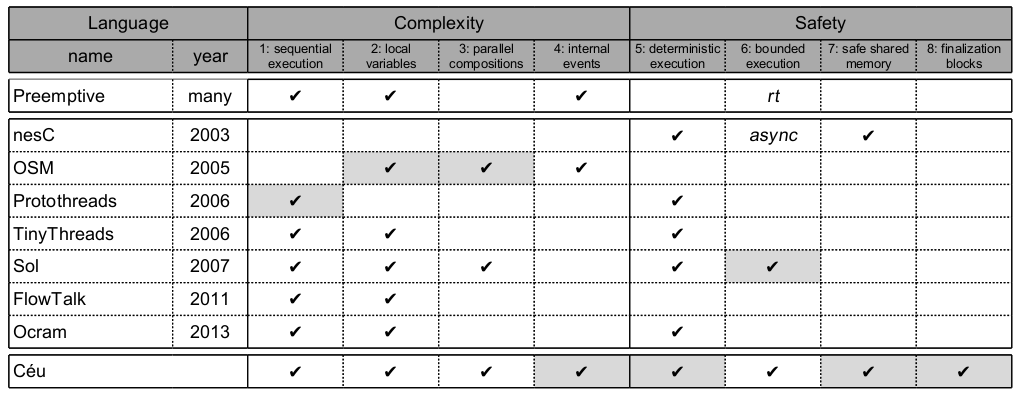
\includegraphics[width=\textwidth,clip=true,trim=110px 340px 120px 0px]{related}
\caption{ Table of features found in work related to \CEU. \newline
{\small %\textmd{
The languages are sorted by the date they first appeared in a publication.
A gray background indicates where the feature first appeared (or a contribution 
if it appears in a \CEU cell).
}%}
\label{fig.related}
}
\end{figure*}

%In this chapter we present~\ref{sec.models} we presented an overview of.

Figure~\ref{fig.related} presents an overview of work related to \CEU, pointing 
out supported features which are grouped by those that reduce complexity and 
those that increase safety.
The line \emph{Preemptive} represents asynchronous languages with preemptive 
scheduling~\cite{wsn.mantisos,wsn.tosthreads}, which are summarized further.
The remaining lines enumerate languages with goals similar to those of \CEU 
that follow a synchronous execution semantics.

Many related approaches allow events to be handled in sequence through a 
blocking primitive, overcoming the main limitation of event-driven systems 
(column~1~\cite{wsn.protothreads, wsn.ocram, wsn.tinythreads, wsn.flowtalk, 
wsn.sol}).
%
As a natural extension, most of them also keep the state of local variables 
between reactions to the environment (column~2).
In addition, \CEU introduces a reliable mechanism to interface local pointers 
with the system through finalization blocks (column~8).
%, as discussed in Section~\ref{sec.ceu.fins}.
%
Given that these approaches use cooperative scheduling, they can provide 
deterministic and reproducible execution (column~5).
%
However, as far as we know, \CEU is the first system to extend this guarantee 
for timers in parallel.

Synchronous languages first appeared in the context of WSNs through 
OSM~\cite{wsn.osm} and Sol~\cite{wsn.sol}, which provide parallel compositions 
(column~3) and distinguish themselves from multi-threaded languages by handling 
thread destruction seamlessly~\cite{sync_async.threadsstop,esterel.preemption}.
Compositions are fundamental for the simpler reasoning about control that made 
possible the safety analysis of \CEU.
%
Sol detects infinite loops at compile time to ensure that programs are 
responsive (column~6).
\CEU adopts the same policy, which first appeared in Esterel.
%
Internal events (column~4) can be used as a reactive alternative to 
shared-memory communication in synchronous languages, as supported in 
OSM~\cite{wsn.osm}.
\CEU introduces a stack-based execution that also provides a restricted but 
safer form of subroutines.
% (as discussed in Section~\ref{sec.ceu.ints}).

\emph{nesC} provides a data-race detector for interrupt handlers (column~7), 
ensuring that \emph{``if a variable x is accessed by asynchronous code, then 
any access of x outside of an atomic statement is a compile-time 
error''}~\cite{wsn.nesc}.
The analysis of \CEU is, instead, targeted at synchronous code and points more 
precisely when accesses can be concurrent, which is only possible because of 
its restricted semantics.
Furthermore, \CEU extends the analysis for system calls (\emph{commands} in 
\emph{nesC}) and control conflicts in trail termination.
Although \emph{nesC} does not enforce bounded reactions, it promotes a 
cooperative style among tasks, and provides asynchronous events that can 
preempt tasks (column 6), something that cannot be done in \CEU.
% (as discussed in Sections~\ref{sec.ceu.det} and \ref{sec.ceu.c}).

On the opposite side of concurrency models, languages with preemptive 
scheduling assume time independence among processes and are more appropriate 
for applications involving algorithmic-intensive problems.
%
Preemptive scheduling is also employed in real-time operating systems to 
provide response predictability, typically through prioritized schedulers
~\cite{wsn.mantisos,wsn.oses,freertos,wsn.tosthreads}.
%
The choice between the two models should take into account the nature of the 
application and consider the trade-off between safe synchronization and 
predictable responsiveness.


%\chapter{Ongoing work}
    %\label{sec.future}
    %TTT

We believe that the design of \CEU make a good tradeoff...

ok on embedded systems

Therefore, our current work with \CEU focus on three main goals:

\begin{itemize}
\item Overcome the limitations of synchronous languages.
\item Become a multi-purpose language.
\item Attract new users.
\end{itemize}

The first...

The second...

\section{Asynchronous execution}

The synchronous computation model of \CEU has some inherent limitations:
%
\begin{itemize}
\item Time-consuming operations break the zero-delay hypothesis of reactions.
      Therefore, \CEU has no support for unbounded loops and blocking C calls 
      (e.g. reading from a socket).
%
\item Input generation is external to the program, making it difficult for a 
      program to simulate its own execution (e.g., for testing purposes).
%
\item Real parallelism is difficult for two reasons:
      the semantics of \CEU is deterministic,
      and the stackless implementation for trails hinders data localization 
      (everything is ``static'').
\end{itemize}

These problems are inherent to the synchronous model and trying to fight them 
by tweaking the language would be a mistake.
%
Our approach is to add support for \emph{asynchronous blocks (asyncs)}, with 
the additional features:
%
\begin{itemize}
\item Can contain unbounded loops.
\item Can make blocking C calls.
\item Can emit input events.
\item Can be parallelizable.
\end{itemize}

Although \emph{asyncs} share the same syntax with \CEU for convenience, they 
can be understood as another language running inside \CEU.
%
In fact, they look much more like $C$ and cannot contain parallel compositions, 
awaits, internal events, finalization blocks, or any synchronous primitive that 
characterizes \CEU.
%
The translation below describes the execution of an \emph{async} from the point 
of view of the synchronous semantics of \CEU:

\begin{figure}[h!]
\begin{minipage}[t]{0.44\linewidth}
\begin{lstlisting}
// asynchronous block
par/or do
    <sync code>
    async do
        <async code>
    end
    <sync code>
with
    <sync code>
end
\end{lstlisting}
\end{minipage}
%
\begin{minipage}[t]{0.56\linewidth}
\begin{lstlisting}
// synchronous interpretation
par/or do
    <sync code>
    emit OUT$_i$;  // spawns <async code>
    await IN$_i$;  // rejoins from <async code>
    <sync code>
with
    <sync code>
end
\end{lstlisting}
\end{minipage}
\end{figure}

In the interpretation, the \code{emit OUT$_i$} makes a non-blocking request to 
start the asynchronous code and is immediately followed by a corresponding 
\code{await IN$_i$}.
%
The \emph{async} runs detached from the \CEU program, which remains responsive 
in the second trail.
%
Once the \emph{async} terminates, it signals \code{IN$_i$} to \CEU (just like a 
normal external event), awaking the first trail.
%
If the second trails terminates before, the \CEU runtime sends an aborting 
signal to the detached \emph{async} (which will never awake the first trail).

Figure~\ref{lst.async.2} shows the implementations in \emph{pthreads} and \CEU 
for a program that makes two heavy calculations in parallel.
%
The \code{par/and} spawns two \emph{asyncs} in parallel, only rejoining after 
they both terminate.
%
The running times in the two implementations are the same, in a duo-core CPU, 
yielding 175\% CPU usage.
%
In terms of implementation, \CEU maps an \emph{async} into a \emph{pthread}, 
using the stack to hold memory and improve data localization.

\begin{figure}[t]
\begin{minipage}[t]{0.37\linewidth}
\begin{lstlisting}
// heavy calculation
void calc () {
 int ret = 0;
 int i, j;
 for (i=0;i<50000;i++)
  for (j=0;j<50000;j++)
   ret += i + j;
 printf("%d\n", ret);
}
\end{lstlisting}
\end{minipage}
%
\begin{minipage}[t]{0.35\linewidth}
\begin{lstlisting}
// pthreads
void main () {
 pth_t t1, t2;
 pth_create(&t1,calc);
 pth_create(&t2,calc);
 pth_join(t1);
 pth_join(t2);
 exit(0);
}


// Time:
// # 17.39s user
// # 175% cpu
\end{lstlisting}
\end{minipage}
%
\begin{minipage}[t]{0.26\linewidth}
\begin{lstlisting}
// Ceu
par/and do
  async do
    _calc();
  end
with
  async do
    _calc();
  end
end

// Time:
// # 17.38s user
// # 175% cpu
\end{lstlisting}
\end{minipage}
\rule{14cm}{0.37pt}
\caption{ A heavy calculation in \CEU with \code{async} blocks.
{\small %\textmd{
}%}
\label{lst.async.2}
}
\end{figure}

\subsection{Simulation}
\label{sec:ceu:simul}

Simulation is an important aspect in cross-compiling platforms, such as 
embedded systems.
It is usually employed to test applications before deploying them on the target 
platform.
%However, simulators are usually inaccurate, varying from platform to platform, 
%and may also require additional knowledge to operate.
%
\CEU can simulate programs in the language itself, not depending on external 
tools.
Given that \emph{asyncs} are allowed to emit input events towards the 
synchronous side of the program, it is easy to simulate and test the execution 
of programs with total control and accuracy with regard to the order of input 
events---all is done with the same language and inside the programs themselves.

\begin{figure}[t]
\begin{minipage}[t]{0.40\linewidth}
\begin{lstlisting}
input int START;
var int v = await START;
par/or do
   loop do
      await 10min;
      v = v + 1;
   end
with
   await 1h35min;
end
\end{lstlisting}
\end{minipage}
%
\begin{minipage}[t]{0.50\linewidth}
\begin{lstlisting}[numbers=left,xleftmargin=-0.5em]
par/or do
   <...> // CODE (in the left)
   _assert(v == 19);
with
   async do
      emit START => 10;
      emit 1h35min;
   end
   _assert(0);
end
\end{lstlisting}
\end{minipage}
\rule{14cm}{0.37pt}
\caption{
A program in the left with a corresponding simulation template in the right.
{\small %\textmd{
}%}
\label{lst.simul}
}
\end{figure}

Suppose we want to simulate the execution of the program in the left of
Figure~\ref{lst.simul}, which initially awaits the input event $START$ (line 2) 
and then increments $v$ every $10$ minutes (lines 4-7) during $1$ hour and $35$ 
minutes (line 7).
%
To test this code, we simulate the occurrence of the event $START$ and the 
passage of \code{1h35min} in a parallel trail, as shown in the right of
Figure~\ref{lst.simul}.
%
The original code remains unmodified and is simply pasted into the template 
(line 2), which runs the simulation in parallel.
%
Note that with a deterministic semantics, a program outcome in \CEU depends 
solely on the events it receives from the environment.
%
The sequence of execution for the simulation is as follows:

{\small
\begin{enumerate}
\setlength{\itemsep}{0pt}
\item The original code initially awaits the event \code{START} (line 2, code 
in the left).
\item The \code{async} (lines 5-9, right) begins, emits \code{START=10} (line 
6, right) and is suspended (synchronous code always have higher priority).
\item The original code resumes and awaits \code{10min} and \code{1h35min} in 
parallel trails (lines 5 and 9, left).
\item The \code{async} resumes and signals that \code{1h35min} has elapsed 
(line 7, right).
\item The original code completely reacts to that: the loop iterates exactly 
$9$ times (lines 4-7, left) before the trail awaiting \code{1h35min} resumes 
(line 9, left) and terminates the innermost \code{par/or}.
The assertion test (line 3, right) executes and terminates the program 
successfully.
The other assertion test (line 9, right) never executes.
\end{enumerate}
}

\begin{comment}
With the proper tools, this integration can be made even simpler (e.g. we 
developed a framework to run tests for the implementation of \CEU{} with 
hundreds of programs and test cases defined in separate).
\end{comment}

It should be clear from the example that simulation does not test true I/O, 
only the program behavior given an arbitrary input sequence.
For instance, the simulation does not take $1$ hour to complete, but actually a 
negligible time.
Also, simulation can be employed---with the exact same behavior---in the 
developing platform or in the target platform.

\begin{comment}
TTT: conclusion?
\subsection{GALS execution}
\label{sec:ceu:gals}

\CEU{} complies with the GALS (\emph{globally asynchronous, locally 
synchronous}) model of computation, which states that local activities run 
synchronized with a common clock, while global activities run with independent 
clocks.
The \emph{globally asynchronous} part of \CEU{} is restricted to external input 
events, $C$ code, and asynchronous blocks, while the \emph{locally synchronous} 
part of \CEU{} extends to all other primitives, such as parallel compositions, 
variable manipulation, and internal events.

The temporal analysis of \CEU{} discussed in Section~\ref{sec:ceu:det} ensures 
that only the locally synchronous part of programs is deterministic.
Therefore, \CEU{} is not an absolutely deterministic language, that is, the 
behavior of programs may vary from execution to execution.

However, nondeterminism in \CEU{} is exclusively a consequence of globally 
asynchronous execution.
For instance, the program in Figure~\ref{lst:ceu:gals} is nondeterministic, 
given that the \code{async} runs for an undetermined time, and may terminate 
before or after the statement \code{await~1s}.
Even so, the \CEU{} compiler does not complain about nondeterminism, because 
the assignments cannot run concurrently.

\begin{figure}[h]
\rule{15cm}{0.37pt}
{\small
\begin{verbatim}
        int ret;
        par/or do
            async do
                ...     // a long computation
            end
            ret = 1;
        with
            await 1s;
            ret = 2;
        end
        return ret;
\end{verbatim}
}
\caption{ The assignments never run concurrently.
\label{lst:ceu:gals}
}
\end{figure}

Note that for simulation purposes, the asynchronous execution can be entirely 
guided by synchronous code, making programs fully deterministic.
For instance, the simulation example of Figure~\ref{lst:ceu:simul:2} can be 
repeated many times, with the exact same behavior.
\end{comment}

\section{Abstractions with ``organisms''}
\label{sec.orgs}

Applications frequently require multiple instances of an abstraction to coexist 
during runtime.
%
%Code reentrancy avoids duplicating code to save ROM, i.e., the same code is 
%shared among instances, which only differ on their data and
%point of execution.
%
In traditional multi-threaded systems, code reentrancy is achieved with 
function declarations that are executed with different stacks and instruction 
pointers.
In object oriented languages, a \emph{class} encapsulates methods and 
properties, and can be instantiated as objects.

In \CEU, we designed an hybrid approach, which combines trails and objects in 
the so called \emph{organisms}.
An organism class is composed of an \emph{interface} and a single \emph{body}.
The interface exposes public variables and internal events that other organisms 
can access.
The body of a class is equivalent to a trail, with all presented functionality 
provided by \CEU, such as parallel compositions, $C$ calls, timers, etc.
An organism is instantiated by declaring a variable of the desired class, and 
its body is automatically spawned in parallel with the enclosing block.

Figure~\ref{lst.orgs} illustrates the use of organisms in \CEU, with an 
application that blinks two LEDs in parallel.
%
The code in the left defines the \code{Blink} class (lines 1-11) exposing the 
\code{led} and \code{freq} variables to be configured by the application (lines 
2,3).
It then initializes to instances (lines 13-16 and 18-21), which start to 
execute their bodies immediately.
%
Once the enclosing block terminates (line 23), both organisms are aborted and 
all memory can be reused.
%
The translation code in the right shows how the organisms bodies are expanded 
to run in a \code{par/or} together with the enclosing block body that 
initializes them (lines 4-8).
The translation is illustrative, i.e., the code is not actually duplicated to 
save memory.
Note that in the expansion, the bodies of the organisms are followed by 
\code{await~FOREVER} (lines 16,24), meaning that only the enclosing block can 
terminate the \code{par/or}.
Note also that the block body runs first and properly initializes the organisms 
before they are spawned, simulating the constructors of organisms.

\begin{figure}[t]
\begin{minipage}[t]{0.45\linewidth}
\begin{lstlisting}
class Blink with
   var int led;
   var int freq;
do
   loop do
      _on(this.led);
      await (this.freq)s;
      _off(this.led);
      await (this.freq)s;
   end
end

var Blink b1 with
    this.led  = 0;
    this.freq = 2;
end;

var Blink b2 with
    this.led  = 1;
    this.freq = 4;
end;

await 1min;
\end{lstlisting}
\end{minipage}
%
\begin{minipage}[t]{0.48\linewidth}
\begin{lstlisting}[numbers=left,xleftmargin=1em]
var _blink_t b1, b2;

par/or do
   b1.led  = 0;
   b1.freq = 2;
   b2.led  = 1;
   b2.freq = 4;
   await 1min;
with
   loop do
      _on(b1.led);
      await (b1.freq)s;
      _off(b1.led);
      await (b1.freq)s;
   end
   await FOREVER;
with
   loop do
      _on(b2.led);
      await (b2.freq)s;
      _off(b2.led);
      await (b2.freq)s;
   end
   await FOREVER;
end
\end{lstlisting}
\end{minipage}
\rule{14cm}{0.37pt}
\caption{ ``Two blinking LEDs'' using organisms.
\label{lst.orgs}
}
\end{figure}

In contrast with objects, note that \CEU organisms are not global entities and 
do not use the heap for memory.
Instead, they are bounded to the scope they are declared, and all memory is 
statically allocated, just like \CEU does with standard local variables.
When an organism goes out of scope, the same automatic bookkeeping of 
\code{par/or} compositions holds, all internal trails are aborted and 
finalization blocks execute (if any).
Hence, the ``garbage collection'' for data and code memory in organisms is 
efficient and static.
%
Methods in \CEU can be simulated by exposing internal events in the class 
interface and all safety guarantees related to bounded memory and execution 
also apply to organisms.

\subsection{Dynamic allocation}

\subsection{New applications}

\begin{figure}[t]
\centering
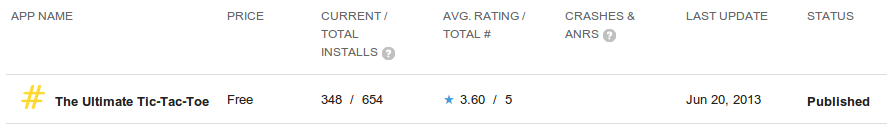
\includegraphics[scale=0.45]{play.png}
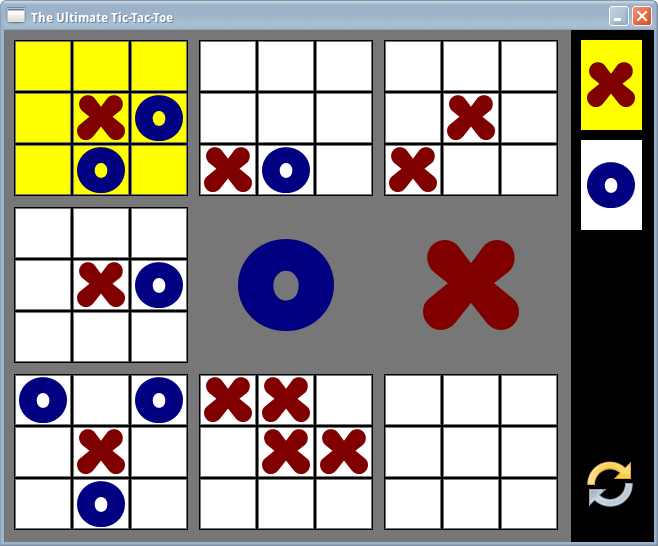
\includegraphics[scale=0.55]{scX.png}
\rule{14cm}{0.37pt}
\caption{ A graphical application in \CEU using the SDL binding.
          The game is published in the ``Android market''.
\label{lst.orgs}
}
\end{figure}

GUI natural
require abstractions, buttons, menus, containers, etc.

- SDL rects
- tic-tac-toe
- networked multi-player game


- nesting
    - data
    - events
    - listeners
    - compositions

- both have an interface
- fields / methods

- fields / internal events
- public fields are ok because reliable shared memory

- no recursive definitions
- but we have interfaces
- special global interface
%end{comment}

\section{Teaching C\'eu}

\subsection{Documentation}
    - wiki, videos, online tutorial

\begin{figure}[t]
\centering
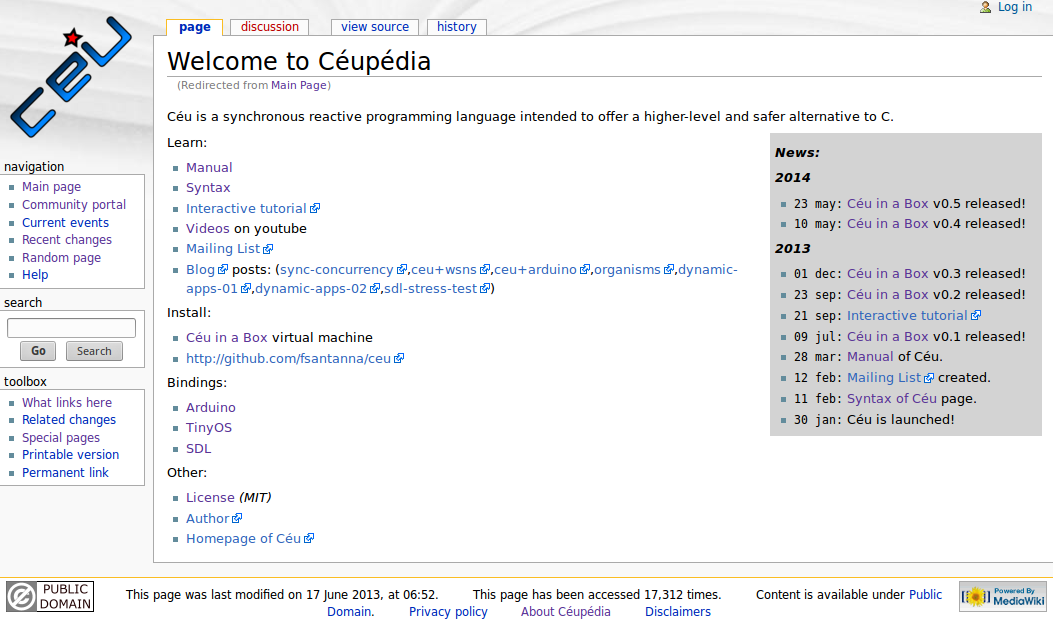
\includegraphics[scale=0.37]{wiki.png}
\rule{14cm}{0.37pt}
\caption{ C\'eup\'edia, the wiki-page of \CEU.
\label{fig.wiki}
}
\end{figure}

\begin{figure}[t]
\centering
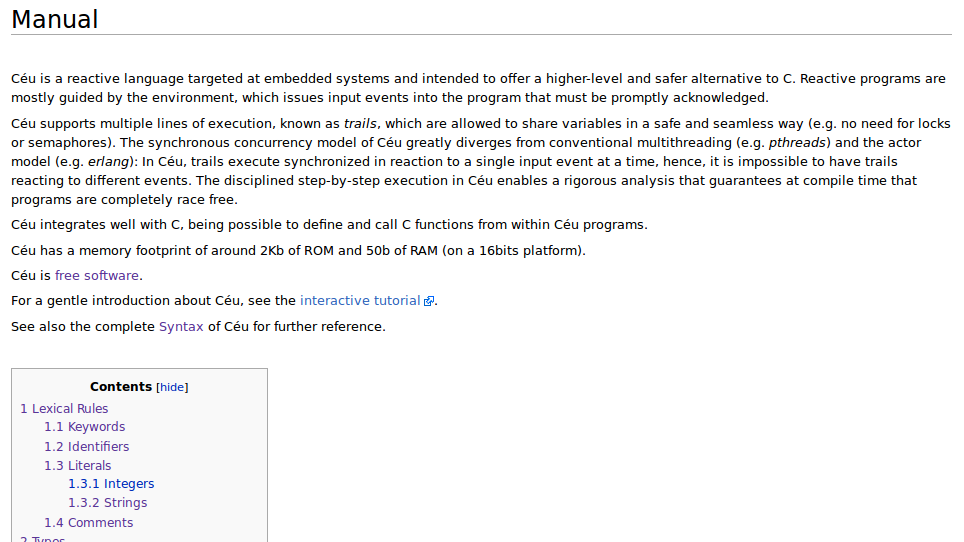
\includegraphics[scale=0.35]{manual.png}
\rule{14cm}{0.45pt}
\caption{ Online manual of \CEU.
\label{fig.wiki}
}
\end{figure}

\begin{figure}[t]
\centering
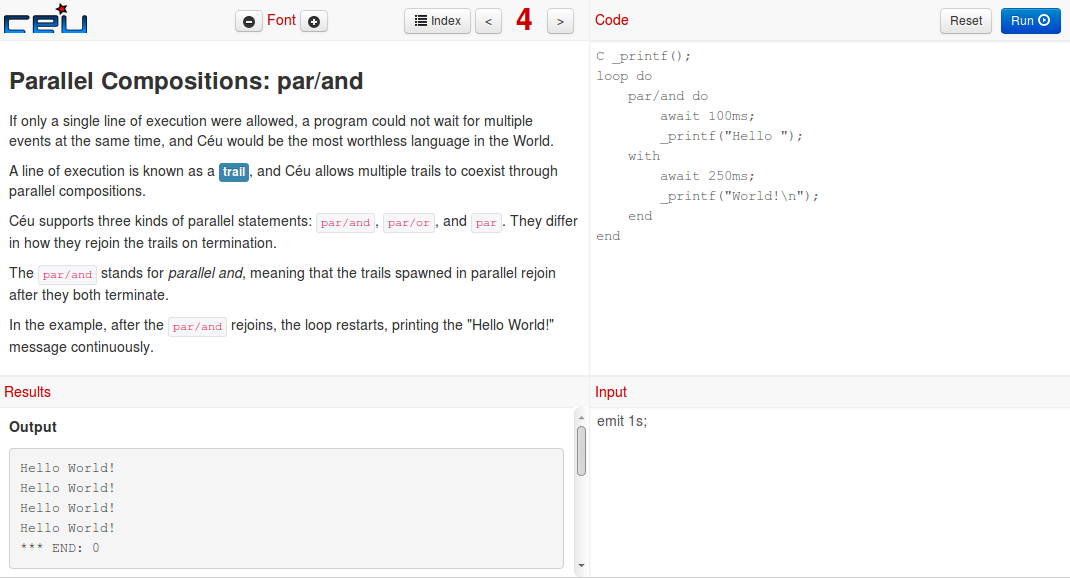
\includegraphics[scale=0.35]{tutorial.png}
\rule{14cm}{0.37pt}
\caption{ Online-interactive tutorial on \CEU. (Thanks to Carlos Mattoso)
\label{fig.tutorial}
}
\end{figure}

\begin{figure}[t]
\centering
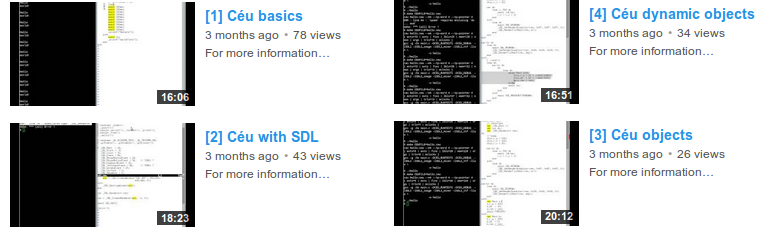
\includegraphics[scale=0.48]{videos.png}
\rule{14cm}{0.37pt}
\caption{ Introductory videos about \CEU.
\label{fig.videos}
}
\end{figure}

\begin{figure}[t]
\centering
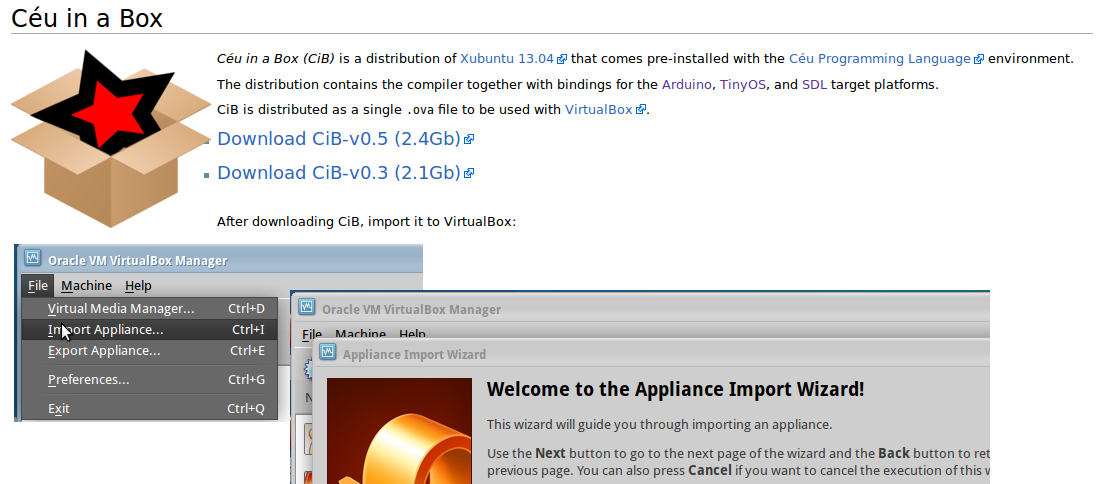
\includegraphics[scale=0.35]{cib.png}
\rule{14cm}{0.37pt}
\caption{ ``C\'eu-in-a-box'': a linux-based VM pre-installed with \CEU for 
TinyOS, Arduino, and SDL.
\label{fig.cib}
}
\end{figure}

\subsection{Classes}
    - puc, ufrj, ort
    - after nesC, they rapidly recognize the gains in productivity with await


\chapter{Conclusion}
    \label{sec.conclusion}
    % TTT: corroborar results dos outros trabalhos

We presented \CEU, a system-level programming language targeting 
control-intensive WSN applications.
\CEU is based on a synchronous core that combines parallel compositions with 
standard imperative primitives, such as sequences, loops and assignments.
%
Our work has three main contributions:
%
\begin{itemize}
%
\item A resource-efficient synchronous language that can express control 
      specifications concisely.
%
\item The stack-based execution policy for internal events as a powerful 
      broadcast communication mechanism.
%
\item A wide set of compile-time safety guarantees for concurrent programs that 
      are still allowed to share memory and access the underlying platform in 
``raw $C$''.
%
\end{itemize}

%
%The static analysis algorithm is actually quite simple and effective .
 %and design decisions that made it possible are quite simple:
%, and obvious if we take for granted the design decisions behind (e.g.
%pushing towards
%The series of decision, discrete execution, uniqueness of events

We argue that the dictated safety mindset of our design does not lead to a 
tedious and bureaucratic programming experience.
%
In fact, the proposed safety analysis actually depends on control information 
that can only be inferred based on high-level control-flow mechanisms (which 
results in more compact implementations).
%
Furthermore, \CEU embraces practical aspects for the context of WSNs, providing 
seamless integration with $C$ and a convenient syntax for timers.
%
%This relationship between safety and expressiveness is two-way, and
%also rely on the safety guarantees to be trustworthy.

As far as we know, \CEU is the first language with stack-based internal events, 
which allows to build rich control mechanisms on top of it, such as a limited 
form of subroutines and exception handling.
%
In particular, \CEU's subroutines compose well with the other control 
primitives and are safe, with guaranteed bounded execution and memory 
consumption.

We presented two complete demos to show how typical patterns in WSNs such as 
sampling, timeout and concurrency can be easily implemented.
They also explore parallel compositions for specifying complementary activities 
in separate.
Communication among activities can either use internal events or safe access to 
global variables.

Our evaluation compares several implementations of widely adopted WSN protocols 
in \CEU to \nesc, showing a considerable reduction in code size with a small 
increase in resource usage.
%
On the way to a more in-depth qualitative approach, such as evaluating the 
leraning curve of the language, we have been teaching \CEU as an alternative to 
\nesc in hands-on WSN courses in a high school for the past two years (and also 
in two universities in short courses).
Our experience shows that students are capable of implementing an 
\emph{SRP}-like routing protocol in \CEU in a couple of weeks.

We presented a formal semantics for the control aspects of \CEU and discussed 
how they are implemented in $C$.
%
The resource-efficient implementation of \CEU is suitable for constrained 
sensor nodes and imposes a small memory overhead in comparison to handcrafted 
event-driven code.

We believe that the strong position in favor of shared-memory concurrency is 
also a contribution of the thesis:
%
first because although synchronous languages emerged in the early eighties, we 
are not aware of derived work allegedly addressing this issue;
%
second because the current trend in the programming-languages community is 
towards the adoption of more pure functional languages and message-passing 
concurrency to get rid of shared memory, which is in the opposite direction of 
\CEU.

%\subsection{Ongoing work}


%\end{comment}

%\bibliographystyle{plain}
\bibliography{my,other}

%\appendix
%\chapter{The Full Semantics of C\'eu}
    %\label{app.formal}
    %%\begin{comment}
\documentclass{article}

\usepackage{amssymb}
\usepackage{amsmath}
\usepackage{amsfonts}
\usepackage{amsthm}
\usepackage{mathtools}

\newcommand{\DS}{\displaystyle}

\newcommand{\ST}{\xrightarrow[~n~]{}}
\newcommand{\BT}{\xRightarrow[(i,E)]{}}

\newcommand{\LL}{\langle}
\newcommand{\RR}{\rangle}

\newcommand{\1}{\;}
\newcommand{\2}{\;\;}
\newcommand{\3}{\;\;\;}
\newcommand{\5}{\;\;\;\;\;}
\newcommand{\ten}{\5\5}
\newcommand{\twenty}{\ten\ten}

\begin{document}
%\end{comment}

\begin{figure}[h]
%\rule{8.5cm}{0.37pt}
{\small
\begin{verbatim}
  // primary statements         // description
  nop(v)                        (constant value)
  mem                           (any memory access)
  await(e)                      (await event `e')
  emit(e,v)                     (emit event `e' passing `v')
  break                         (loop escape)

  // compound statements
  if mem then p else q          (conditional)
  p ; q                         (sequence)
  loop p                        (repetition)
  p and q                       (par/and)
  p or q                        (par/or)

  // derived by semantic rules
  awaiting(e,m)                 (awaiting `e' since sequence number `m')
  emitting(t)                   (emitting on stack level `t')
  p @ loop p                    (unwinded loop)
\end{verbatim}
}%
\end{figure}

$$
\LL S, s, p \RR
    \xrightarrow[~~n~~]{~~*~~}
\LL S', s', p' \RR
$$

\begin{figure}[h!]
{\small
\begin{align*}
  isBlocked(n,S,s, awaiting(e,m)) &= (e \neq S(s) \1\vee\1 m = n)   \\
  isBlocked(n,S,s, emitting(t))   &= (t \neq s)                     \\
  isBlocked(n,S,s, (p~;~q))       &= isBlocked(n,S,s,p)             \\
  isBlocked(n,S,s, (p~@~loop~q))  &= isBlocked(n,S,s,p)             \\
  isBlocked(n,S,s, (p~and~q))     &= isBlocked(n,S,s,p) \wedge
                                     isBlocked(n,S,s,q)             \\
  isBlocked(n,S,s, (p~or~q))      &= isBlocked(n,S,s,p) \wedge
                                     isBlocked(n,S,s,q)             \\
  isBlocked(n,S,s, *)             &= false \2  (nop,mem,await,      \\
                                  &    \5\5\5\2 emit,break,if,loop)   %\\
\end{align*}
}%
\end{figure}

\begin{figure}[h!]
{\small
\begin{align*}
  clear( awaiting(\epsilon,m)~;~q ) &= q                   \\
  clear( p~;~q )                    &= clear(p)            \\
  clear( p~@~loop~q) )              &= clear(p)            \\
  clear( p~and~q )                  &= clear(p)~;~clear(q) \\
  clear( p~or~q )                   &= clear(p)~;~clear(q) \\
  clear( * )                        &= nop(0)
\end{align*}
}%
\end{figure}

\begin{align*}
\LL S,s, mem \RR &\ST
\LL S,s, nop(v) \RR,~~(v~is~nondet)
    & \textbf{(mem)}        \\
%%%
\LL S,s, await(e) \RR &\ST
\LL S,s, awaiting(e,n) \RR
    & \textbf{(await)}      \\
%%%
\LL S,s, emit(e,v) \RR &\ST
\LL S \uplus \{(s+1) \mapsto e\},s+1, mem~;~emitting(s) \RR
    & \textbf{(emit)}       \\
%%%
\LL S,s, awaiting(S(s),m) \RR &\ST
\LL S,s, mem \RR, m<n
    & \textbf{(awaiting)}   \\
%%%
\LL S,s, emitting(s) \RR &\ST
\LL S,s, nop(1) \RR
    & \textbf{(emitting)}   \\
\end{align*}

\begin{eqnarray*}
& \frac
    {\DS isBlocked(p) \1\wedge\1 s>=0 }
% -----------------------------------------------------------
    {\DS \LL S,s, p \RR \ST \LL S,s-1,p \RR }
    & \textbf{(pop)}       \\
%%%
& \frac
    {\DS m \ST m' }
% -----------------------------------------------------------
    {\DS \LL S,s, (if~m~then~p~else~q) \RR \ST
         \LL S,s, (if~m'~then~p~else~q)\RR }
    & \textbf{(if-adv)}       \\
%%%
& \LL S,s, (if~nop(v)~then~p~else~q) \RR \ST
  \LL S,s,  p \RR \1,\3 (v \neq 0)
    & \textbf{(if-true)}       \\
%%%
& \LL S,s, (if~nop(0)~then~p~else~q) \RR \ST
  \LL S,s, q \RR
    & \textbf{(if-false)}       \\
%%%
& \frac
    {\DS p \ST p' }
%   -----------------------------------------------------------
    {\DS \LL S,s, (p~;~q) \RR \ST \LL S,s, (p'~;~q) \RR }
    & \textbf{(seq-adv)}      \\
%%%
& \LL S,s, (nop~;~q) \RR \ST  \LL S,s, q \RR
    & \textbf{(seq-cst)}      \\
%%%
& \LL S,s, (break~;~q) \RR \ST \LL S,s, break \RR
    & \textbf{(seq-brk)}      \\
%%%
& \LL S,s, (loop~p) \RR \ST \LL S,s, (p~@~loop~p) \RR
    & \textbf{(loop-expd)}       \\
%%%
& \frac
    {\DS p \ST p' }
% -----------------------------------------------------------
    {\DS \LL S,s, (p~@~loop~q) \RR \ST \LL S,s, (p'~@~loop~q) \RR }
    & \textbf{(loop-adv)}    \\
%%%
& \LL S,s, (nop~@~loop~p) \RR \ST \LL S,s, loop~p \RR
    & \textbf{(loop-cst)}    \\
%%%
& \LL S,s, (break~@~loop~p) \RR \ST \LL S,s, nop \RR
    & \textbf{(loop-brk)}    \\
%%%
& \frac
    {\DS p \ST p' }
%   -----------------------------------------------------------
    {\DS \LL S,s, (p~and~q) \RR \ST \LL S,s, (p'~and~q) \RR }
    & \textbf{(and-adv1)}      \\
%%%
& \frac
    {\DS isBlocked(p) \1\wedge\1 q \ST q' }
%   -----------------------------------------------------------
    {\DS \LL S,s, (p~and~q) \RR \ST \LL S,s, (p~and~q') \RR }
    & \textbf{(and-adv2)}      \\
%%%
& \LL S,s, (nop~and~q) \RR \ST \LL S,s, q \RR
    & \textbf{(and-nop1)}   \\
%%%
& \LL S,s, (p~and~nop) \RR \ST \LL S,s, p \RR
    & \textbf{(and-nop2)}   \\
%%%
& \LL S,s, (break~and~q) \RR \ST \LL S,s, (clear(q)~;~break) \RR
    & \textbf{(and-brk1)}   \\
%%%
& \frac
    {\DS isBlocked(p) }
%   -----------------------------------------------------------
    {\DS \LL S,s, (p~and~break) \RR \ST \LL S,s, (clear(p)~;~break) \RR }
    & \textbf{(and-brk2)}   \\
%%%
& \frac
    {\DS p \ST p' }
%   -----------------------------------------------------------
    {\DS \LL S,s, (p~or~q) \RR \ST \LL S,s, (p'~or~q) \RR }
    & \textbf{(or-adv1)}   \\
%%%
& \frac
    {\DS isBlocked(p) \1\wedge\1 q \ST q' }
%   -----------------------------------------------------------
    {\DS \LL S,s (p~or~q) \RR \ST \LL S,s, (p~or~q') \RR }
    & \textbf{(or-adv2)}   \\
%%%
& \LL S,s, (nop~or~q) \RR \ST \LL S,s, clear(q) \RR
    & \textbf{(or-nop1)}   \\
%%%
& \frac
    {\DS isBlocked(p) }
%   -----------------------------------------------------------
    {\DS \LL S,s, (p~or~nop) \RR \ST \LL S,s, (clear(p)~;~break) \RR }
    & \textbf{(or-nop2)}   \\
%%%
& \LL S,s, (break~or~q) \ST \LL S,s, clear(q) \RR
    & \textbf{(or-brk1)}   \\
%%%
& \frac
    {\DS isBlocked(p) }
%   -----------------------------------------------------------
    {\DS \LL S,s, (p~or~break) \RR \ST \LL S,s, (clear(p)~;~break) \RR }
    & \textbf{(or-brk2)}   %\\
\end{eqnarray*}

\end{document}


\end{document}
